\documentclass[12pt, letterpaper]{article}

% -------------------------------------------------
% PAQUETES Y FORMATO
% -------------------------------------------------
\usepackage[utf8]{inputenc}
\usepackage[T1]{fontenc}
\usepackage[spanish,mexico]{babel}
\usepackage{amsmath,amssymb,amsfonts}
\usepackage[margin=2.5cm,top=2.5cm,bottom=2.5cm]{geometry}
\usepackage{helvet}
\renewcommand{\familydefault}{\sfdefault}
\usepackage{enumitem}
\usepackage{graphicx}
\usepackage{float}
\usepackage{array,booktabs}
\usepackage{tikz}
\usepackage{fancyhdr}
\usepackage{lastpage}
\usepackage{titlesec}
\usepackage{xcolor}
\usepackage{tcolorbox}
% La expansión automática de microtype falla con la fuente monoespaciada
% usada por los marcadores de gráficas en algunas instalaciones de MiKTeX.
\usepackage[expansion=false]{microtype}
\usepackage{hyperref}

% El cuadernillo numera los incisos con el alfabeto latino sin incluir la ñ.
\makeatletter
\renewcommand{\alph}[1]{\expandafter\@alphlatin\csname c@#1\endcsname}
\newcommand{\@alphlatin}[1]{\ifcase#1\or a\or b\or c\or d\or e\or f\or g\or h\or i\or j\or k\or l\or m\or n\or o\or p\or q\or r\or s\or t\or u\or v\or w\or x\or y\or z\else\@ctrerr\fi}
\makeatother

\definecolor{MoradoPrincipal}{RGB}{74,20,140}
\definecolor{MoradoSecundario}{RGB}{106,27,154}
\definecolor{MoradoClaro}{RGB}{243,229,245}
\definecolor{GrisTexto}{RGB}{33,33,33}

\setlength{\parindent}{0pt}
\setlength{\parskip}{5pt}
\setlength{\emergencystretch}{2em}
\setlength{\headheight}{14.5pt}
\setlist[enumerate]{itemsep=0.45em,topsep=0.35em}
\setlist[itemize]{itemsep=0.25em,topsep=0.3em}

\pagestyle{fancy}
\fancyhf{}
\fancyhead[L]{\small\color{GrisTexto} Cálculo Diferencial}
\fancyhead[R]{\small\color{GrisTexto} Cuadernillo resuelto}
\fancyfoot[C]{\small\color{GrisTexto} Página \thepage\ de \pageref{LastPage}}
\renewcommand{\headrulewidth}{0.6pt}
\renewcommand{\footrulewidth}{0.4pt}
\renewcommand{\headrule}{{\color{MoradoPrincipal}\hrule width\headwidth height \headrulewidth \vspace{-\headrulewidth}}}
\renewcommand{\footrule}{{\color{MoradoPrincipal}\hrule width\headwidth height \footrulewidth \vspace{-\footrulewidth}}}

\titleformat{\section}
  {\color{MoradoPrincipal}\normalfont\Large\bfseries}
  {\thesection.}{0.5em}{}
  [\color{MoradoPrincipal}\titlerule]

\titleformat{\subsection}
  {\color{MoradoSecundario}\normalfont\large\bfseries}
  {\thesubsection.}{0.5em}{}

\titleformat{\subsubsection}
  {\color{MoradoPrincipal}\normalfont\bfseries}
  {\thesubsubsection.}{0.5em}{}

\hypersetup{
    colorlinks=true,
    linkcolor=MoradoPrincipal,
    filecolor=MoradoSecundario,
    urlcolor=MoradoPrincipal,
    pdftitle={Cuadernillo resuelto: Cálculo diferencial},
    pdfauthor={Rodríguez Rodríguez Diego Felipe}
}

% Cada llamada conserva el espacio destinado a una evidencia, con el diseño
% visual de Tarea 4.
\newcommand{\grafica}{%
    \begin{center}
        \begin{tcolorbox}[
            colframe=MoradoPrincipal,
            colback=MoradoClaro!30,
            arc=3mm,
            width=0.86\textwidth,
            height=2.3cm,
            halign=center,
            valign=center
        ]
            \texttt{// evidencia de gráfica}
        \end{tcolorbox}
    \end{center}
}

\newcommand{\R}{\mathbb{R}}

\newcommand{\sen}{\operatorname{sen}}

\newcommand{\arcsec}{\operatorname{arcsec}}

\newcommand{\sgn}{\operatorname{sgn}}

\newcommand{\respuesta}[1]{\[\boxed{#1}\]}

% Colores originales de las gráficas de Desmos
\definecolor{desmosMorado}{HTML}{975FA8}
\definecolor{desmosAzulFuerte}{HTML}{6557D2}
\definecolor{desmosAzul}{HTML}{1565C0}
\definecolor{desmosVerde}{HTML}{388C83}
\definecolor{desmosAmarillo}{HTML}{FFCC02}
\definecolor{desmosRojo}{HTML}{D32F2F}

\begin{document}

\begin{titlepage}
    \thispagestyle{empty}
    \begin{center}
        \begin{table}[h!]
            \centering
            \begin{tabular}{m{3.5cm} m{8cm} m{3.5cm}}
                \centering
                \IfFileExists{../Logos/unam_logo.png}
                {\includegraphics[width=3cm,height=3.5cm,keepaspectratio]{../Logos/unam_logo.png}}
                {\framebox{\parbox[c][3.5cm][c]{3cm}{\centering UNAM}}}
                &
                \centering
                {\bfseries\large UNIVERSIDAD NACIONAL AUTÓNOMA DE MÉXICO}\\[0.3cm]
                {\bfseries\large FACULTAD DE ESTUDIOS SUPERIORES ARAGÓN}\\[0.2cm]
                {\small\color{MoradoPrincipal}\rule{8cm}{1.5pt}}
                &
                \centering
                \IfFileExists{../Logos/fes_aragon_logo.png}
                {\includegraphics[width=3.5cm,height=3.5cm,keepaspectratio]{../Logos/fes_aragon_logo.png}}
                {\framebox{\parbox[c][3.5cm][c]{3.5cm}{\centering FES Aragón}}}
            \end{tabular}
        \end{table}

        \vspace{1.5cm}
        {\color{MoradoPrincipal}\Large\bfseries INGENIERÍA EN COMPUTACIÓN}\\[0.4cm]
        {\color{MoradoSecundario}\large\bfseries Cálculo diferencial}\\[1.5cm]

        \begin{tcolorbox}[
            colframe=MoradoPrincipal,
            colback=MoradoClaro!30,
            arc=3mm,
            width=0.9\textwidth,
            halign=center
        ]
            \vspace{0.3cm}
            {\large\bfseries Cuadernillo resuelto}\\[0.2cm]
            \small Ejercicios, procedimientos y evidencias de cálculo diferencial.
            \vspace{0.3cm}
        \end{tcolorbox}

        \vfill
        \begin{table}[h!]
            \centering
            \begin{tabular}{rl}
                \textbf{\color{MoradoPrincipal} Alumno:} & Rodríguez Rodríguez Diego Felipe\\[0.2cm]
                \textbf{\color{MoradoPrincipal} Profesor:} & Dr. Arturo Rodríguez García\\[0.2cm]
                \textbf{\color{MoradoPrincipal} Asignatura:} & Cálculo diferencial\\[0.2cm]
                \textbf{\color{MoradoPrincipal} Trabajo:} & Cuadernillo de ejercicios\\[0.2cm]
            \end{tabular}
        \end{table}

        \vspace{1cm}
        {\small San Juan de Aragón, Estado de México}
    \end{center}
\end{titlepage}

\newpage
\pagenumbering{arabic}
\setcounter{page}{2}
\renewcommand{\contentsname}{\color{MoradoPrincipal} ÍNDICE GENERAL}
\tableofcontents

\newpage

% =================================================
% TEMA 1
% =================================================
\section{Tema 1. Funciones}

\subsection*{1.- Encuentra el dominio y rango de las siguientes funciones. Muestra la gráfica de la función.}
\begin{enumerate}[label=\alph*)]
  \item $y=2x-3$.\begin{center}
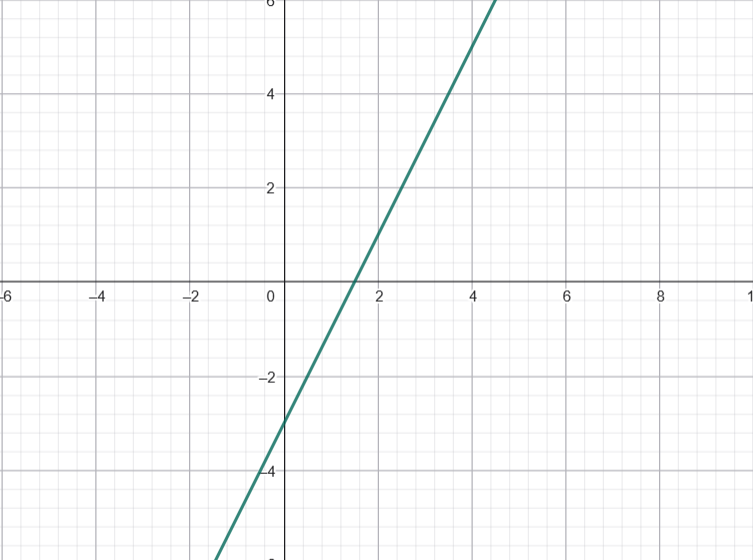
\includegraphics[width=0.86\textwidth]{imagenes/tema1_1_a.png}
\end{center}
  \textbf{Dominio: }$\R$. \quad \textbf{Rango: }$\R$.
  \item $y=x^2+1$.\begin{center}
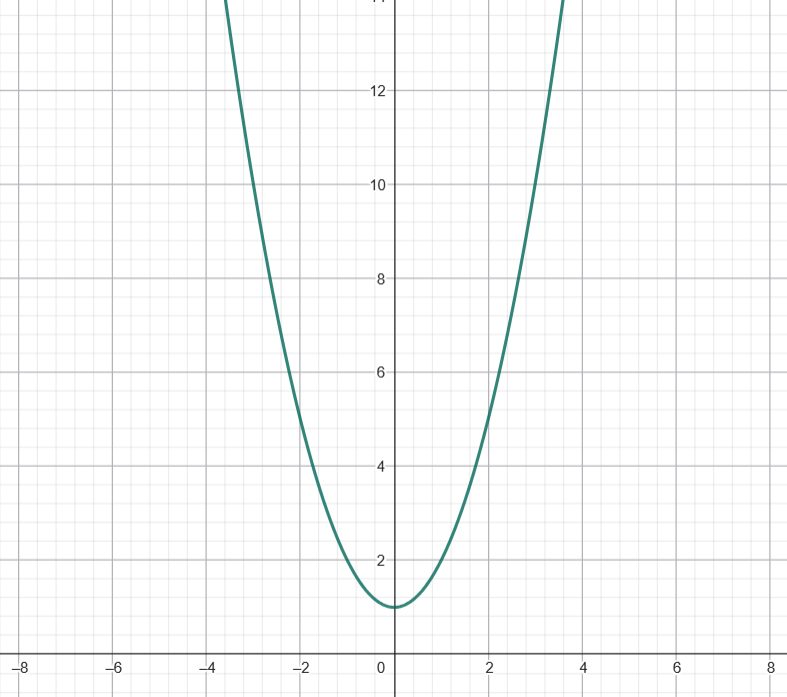
\includegraphics[width=0.86\textwidth]{imagenes/tema1_1_b.png}
\end{center}
  \textbf{Dominio: }$\R$. \quad \textbf{Rango: }$[1,+\infty)$, pues $x^2\geq0$.
  \item $y=\sqrt{x-2}$.\begin{center}
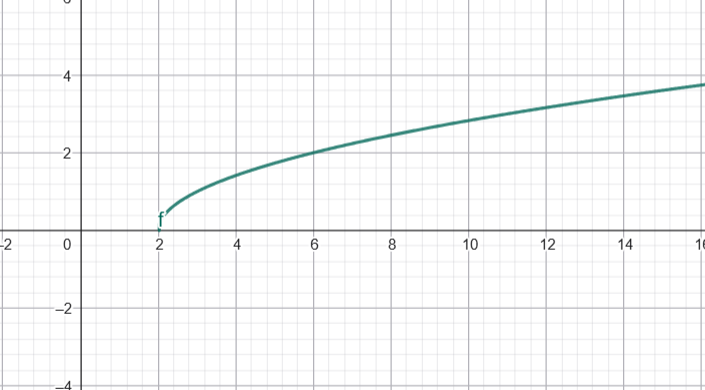
\includegraphics[width=0.86\textwidth]{imagenes/tema1_1_c.png}
\end{center}
  Para que la raíz sea real, $x-2\geq0$.\\
  \textbf{Dominio: }$[2,+\infty)$. \quad \textbf{Rango: }$[0,+\infty)$.
  \item $y=\dfrac{1}{x+3}$.\begin{center}
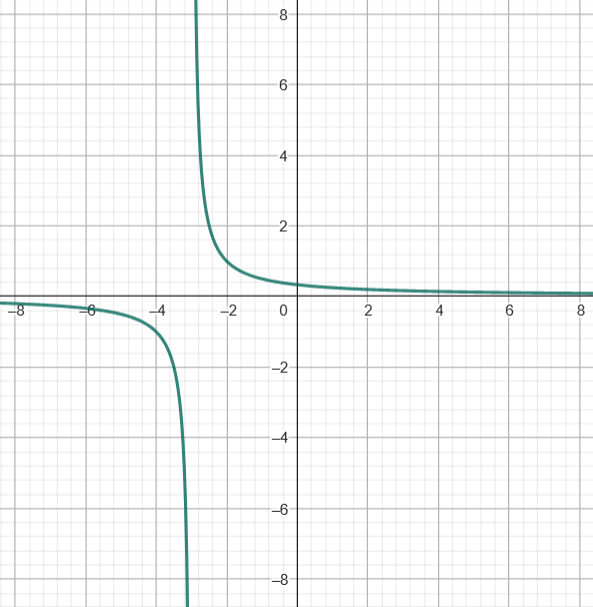
\includegraphics[width=0.86\textwidth]{imagenes/tema1_1_d.png}
\end{center}
  El denominador no puede ser cero: $x\neq-3$. Además, la fracción nunca vale cero.\\
  \textbf{Dominio: }$\R\setminus\{-3\}$. \quad \textbf{Rango: }$\R\setminus\{0\}$.
  \item $y=x^3+2$.\begin{center}
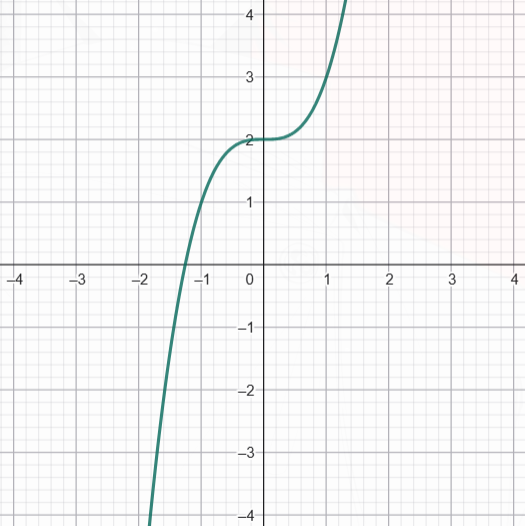
\includegraphics[width=0.86\textwidth]{imagenes/tema1_1_e.png}
\end{center}
  \textbf{Dominio: }$\R$. \quad \textbf{Rango: }$\R$.
\end{enumerate}

\subsection*{2.- Encuentra el dominio de las siguientes funciones. Muestra la gráfica de la función.}
\begin{enumerate}[label=\alph*)]
  \item $y=\dfrac{1}{x^2-9}$.\begin{center}
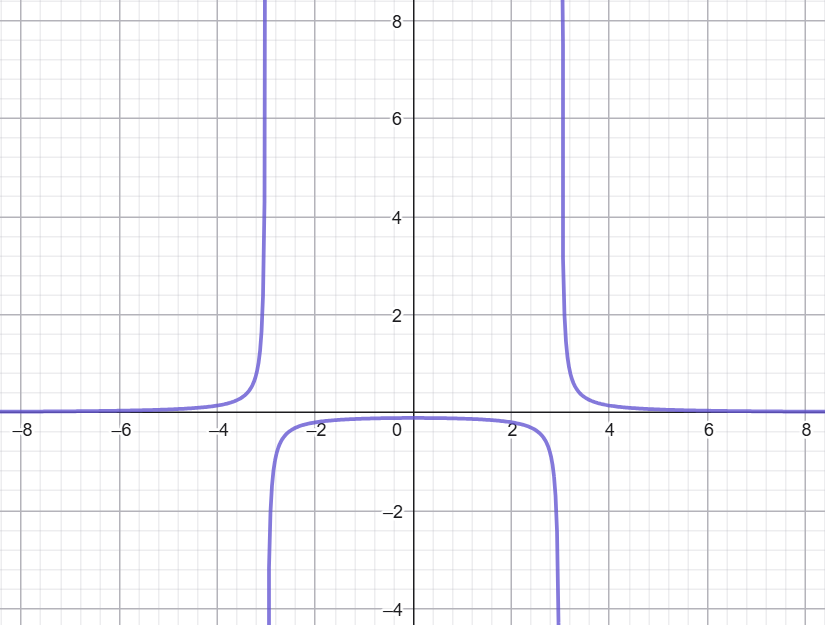
\includegraphics[width=0.86\textwidth]{imagenes/tema1_2_a.png}
\end{center}
  $x^2-9=(x-3)(x+3)\neq0$. \respuesta{D=(-\infty,-3)\cup(-3,3)\cup(3,+\infty)}
  \item $y=\dfrac{1}{x^2-5x+6}$.\begin{center}
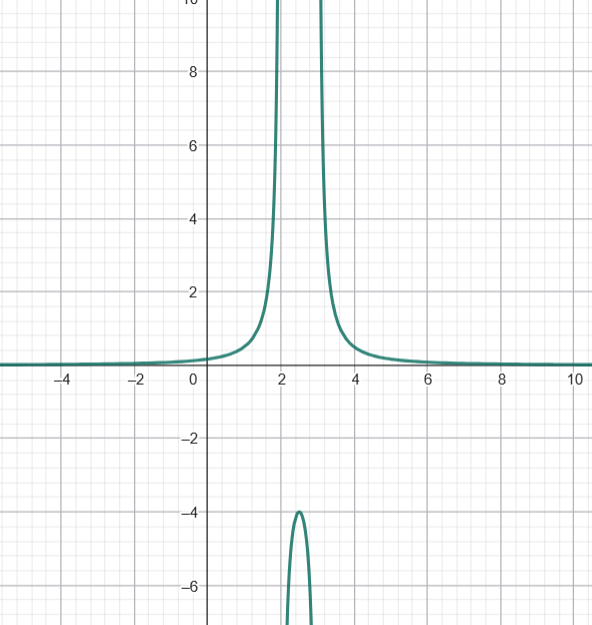
\includegraphics[width=0.86\textwidth]{imagenes/tema1_2_b.png}
\end{center}
  $x^2-5x+6=(x-2)(x-3)\neq0$. \respuesta{D=\R\setminus\{2,3\}}
  \item $y=\dfrac{1}{x^2+6x+9}$.\begin{center}
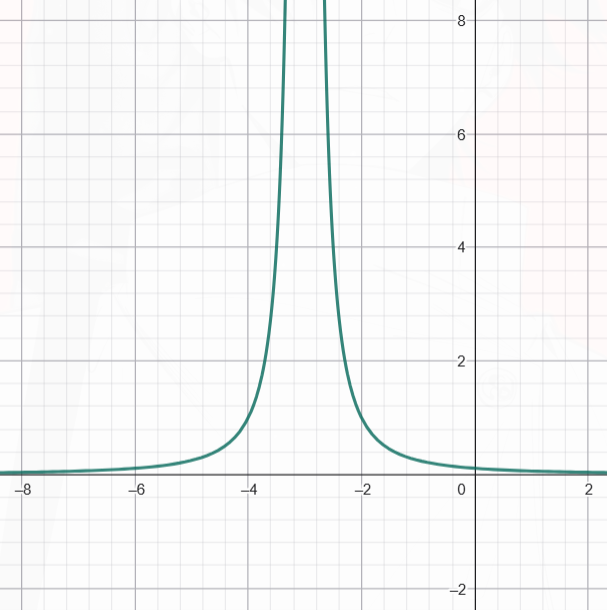
\includegraphics[width=0.86\textwidth]{imagenes/tema1_2_c.png}
\end{center}
  $x^2+6x+9=(x+3)^2\neq0$. \respuesta{D=\R\setminus\{-3\}}
  \item $y=\dfrac{1}{x^2-x-6}$.\begin{center}
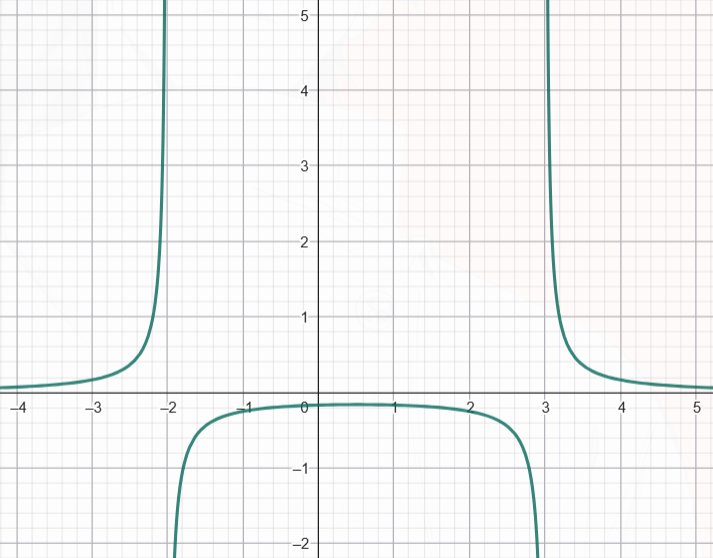
\includegraphics[width=0.86\textwidth]{imagenes/tema1_2_d.png}
\end{center}
  $x^2-x-6=(x-3)(x+2)\neq0$. \respuesta{D=\R\setminus\{-2,3\}}
  \item $y=\dfrac{\sqrt{x}}{x^2-x-6}$.\begin{center}
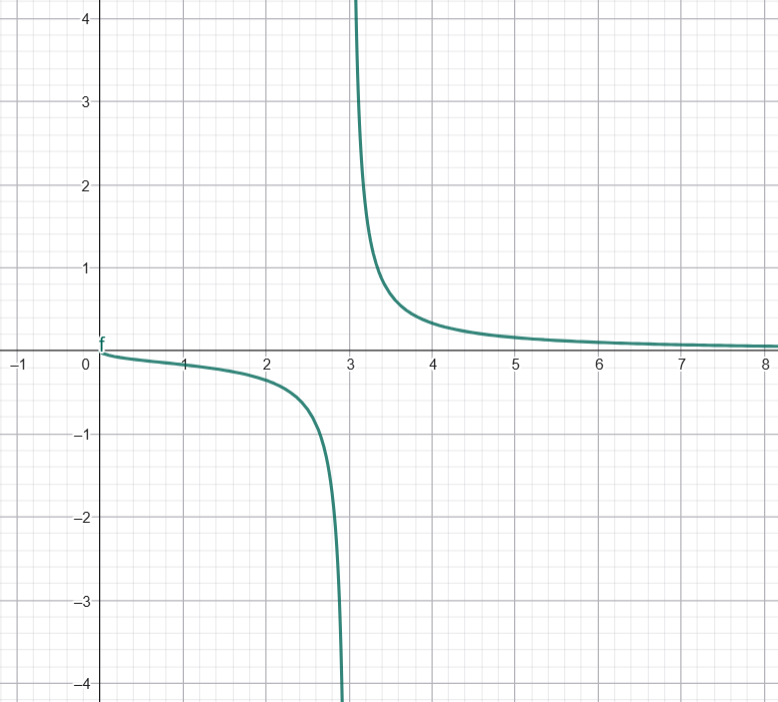
\includegraphics[width=0.86\textwidth]{imagenes/tema1_2_e.png}
\end{center}
  Se requiere $x\geq0$ y $(x-3)(x+2)\neq0$. Al intersectar las condiciones: 
  \respuesta{D=[0,3)\cup(3,+\infty)}
\end{enumerate}

\subsection*{3.- Muestre la gráfica de las siguientes funciones seccionadas}
\begin{enumerate}[label=\alph*)]
  \item $f(x)=\begin{cases}x^2,&\text{si }x<2,\\x+6,&\text{si }x\geq2.\end{cases}$
  \begin{center}
  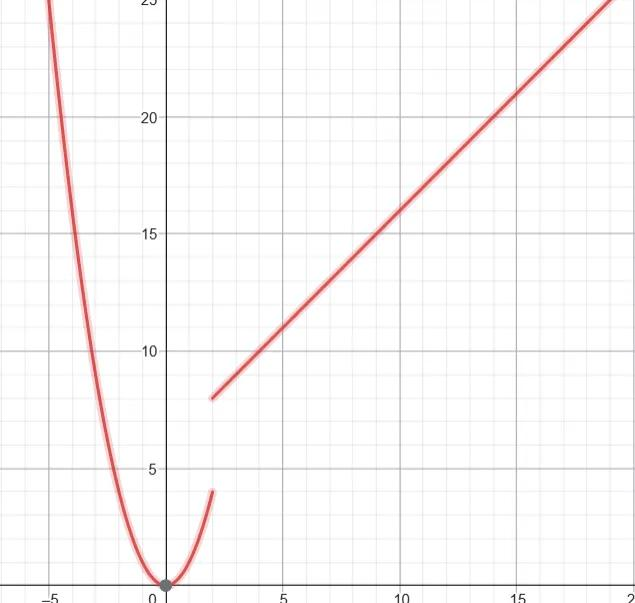
\includegraphics[width=0.86\textwidth]{imagenes/tema1_3_a.jpeg}
  \end{center}
  \item $f(x)=\begin{cases}x^2,&\text{si }x\leq2,\\x+6,&\text{si }x>2.\end{cases}$
  \begin{center}
  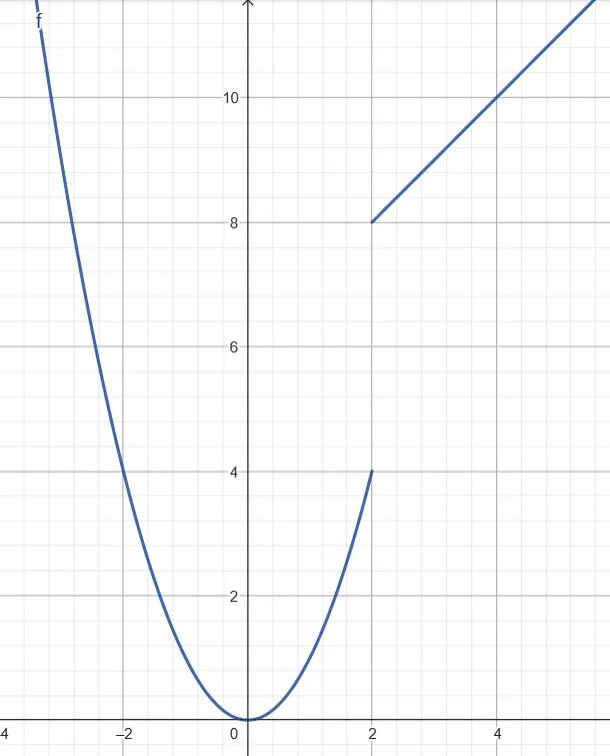
\includegraphics[width=0.86\textwidth]{imagenes/tema1_3_b.jpeg}
  \end{center}
  \item $f(x)=\begin{cases}x^2,&\text{si }x<2,\\x+6,&\text{si }x>2.\end{cases}$
  \begin{center}
  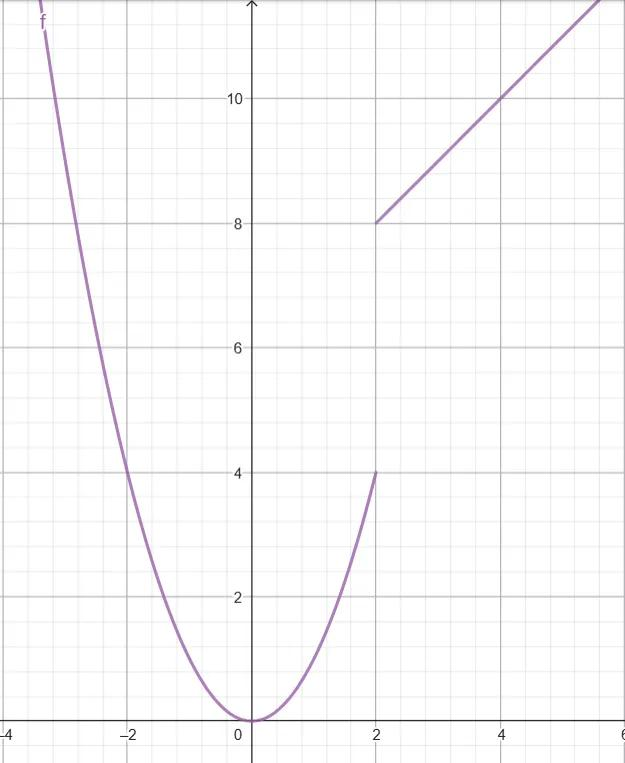
\includegraphics[width=0.86\textwidth]{imagenes/tema1_3_c.jpeg}
  \end{center}
  \item $f(x)=\begin{cases}x^2,&\text{si }x<2,\\6,&\text{si }x=2,\\x+6,&\text{si }x>2.\end{cases}$
  \begin{center}
  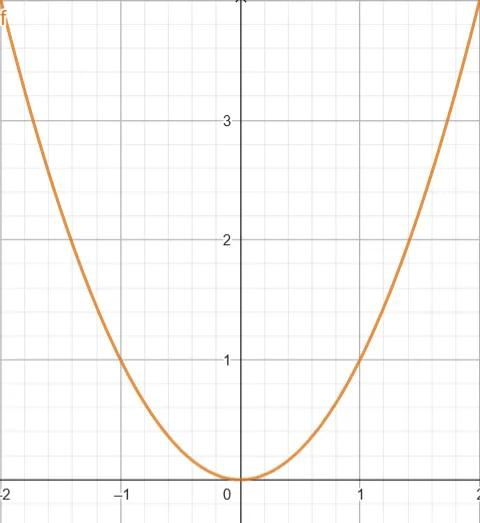
\includegraphics[width=0.86\textwidth]{imagenes/tema1_3_d.jpeg}
  \end{center}
  \newpage
  \item $f(x)=\begin{cases}-1,&\text{si }x\leq0,\\1,&\text{si }0<x<3,\\2,&\text{si }x\geq3.\end{cases}$
  \begin{center}
  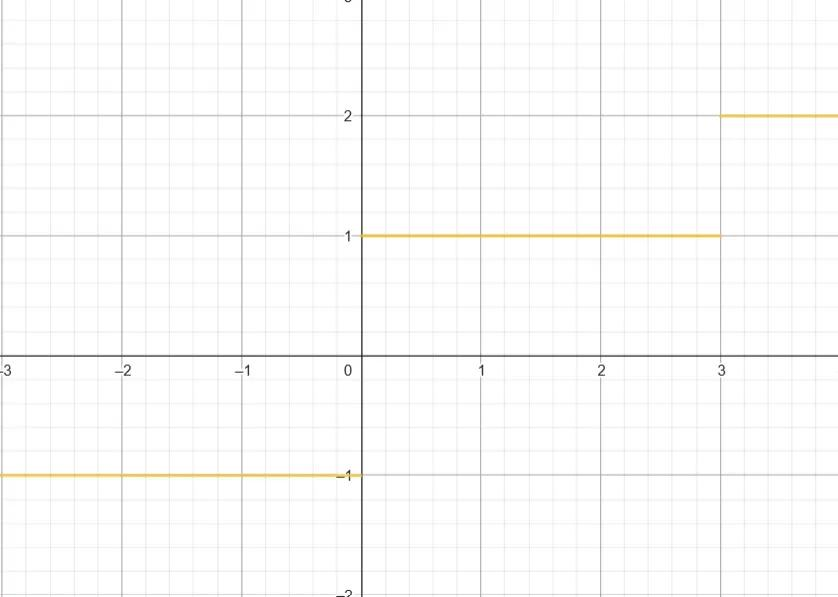
\includegraphics[width=0.86\textwidth]{imagenes/tema1_3_e.jpeg}
  \end{center}
\end{enumerate}

\subsection*{4.- Para las siguientes funciones, indica si se trata de una función par, una función impar, o ninguna de las anteriores.}
\begin{enumerate}[label=\alph*)]
  \item $f(x)=x^4$. Como $f(-x)=(-x)^4=x^4=f(x)$, \textbf{es par}.
  \item $f(x)=\dfrac1x$. Como $f(-x)=\dfrac1{-x}=-\dfrac1x=-f(x)$, \textbf{es impar}.
  \item $f(x)=x+1$. $f(-x)=-x+1$, que no es igual a $f(x)$ ni a $-f(x)$. \textbf{No es par ni impar}.
  \item $f(x)=x$. $f(-x)=-x=-f(x)$, \textbf{es impar}.
  \item $f(x)=\dfrac1{x^2}$. $f(-x)=\dfrac1{(-x)^2}=\dfrac1{x^2}=f(x)$, \textbf{es par}.
\end{enumerate}

\subsection*{5.- Para las siguientes funciones, indica los intervalos en que son crecientes y los intervalos en que son decrecientes.}
\begin{enumerate}[label=\alph*)]
  \item $f(x)=-3x+2$. Pendiente negativa: \textbf{decreciente en }$(-\infty,+\infty)$.
  \item $f(x)=x^3$. \textbf{Creciente en }$(-\infty,+\infty)$.
  \item $f(x)=x^2+4$. \textbf{Decreciente en }$(-\infty,0]$ y \textbf{creciente en }$[0,+\infty)$.
  \item $f(x)=-|x|=\begin{cases}x,&x<0,\\-x,&x\geq0.\end{cases}$ \textbf{Creciente en }$(-\infty,0]$ y \textbf{decreciente en }$[0,+\infty)$.
  \item $f(x)=5$. Es constante en $\R$; no es estrictamente creciente ni estrictamente decreciente (es no decreciente y no creciente a la vez).
\end{enumerate}

% =================================================
% TEMA 2
% =================================================

\newpage
\section{Tema 2. Funciones algebraicas y funciones trascendentes}

Utiliza un graficador para mostrar las gráficas de las siguientes funciones. Puedes colocar varias funciones en un mismo plano cartesiano siempre y cuando se distingan claramente una de la otra (por ejemplo, ponerlas con diferentes colores).

\subsection*{FUNCIONES ALGEBRAICAS}
\subsubsection*{1.- Funciones constantes}
\begin{itemize}[label=\quad, leftmargin=*, itemsep=0.5em]
  \item[\textcolor{desmosMorado}{$\blacksquare$}] $y=4$
  \item[\textcolor{desmosAzulFuerte}{$\blacksquare$}] $y=2$
  \item[\textcolor{desmosAzul}{$\blacksquare$}] $y=-2$
  \item[\textcolor{desmosVerde}{$\blacksquare$}] $y=-5$
  \item[\textcolor{desmosAmarillo}{$\blacksquare$}] $y=0$
\end{itemize}
\begin{center}
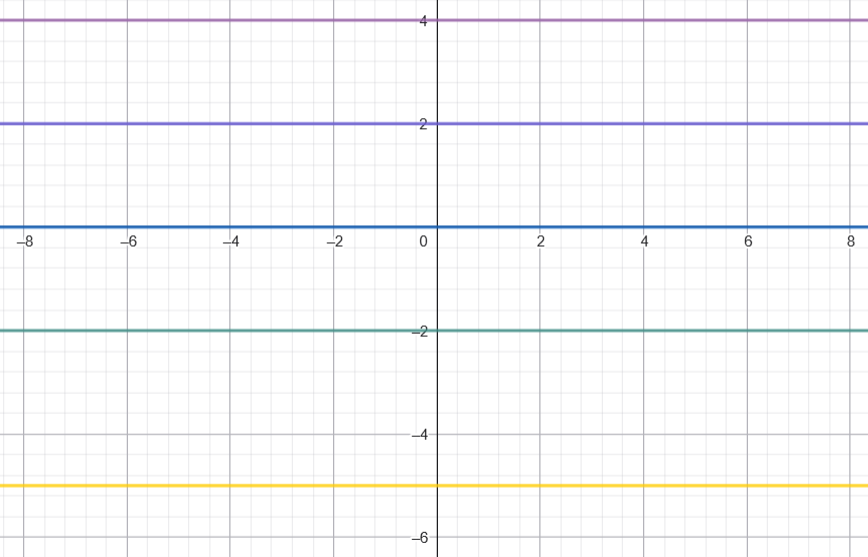
\includegraphics[width=0.86\textwidth]{imagenes/tema2_constantes.png}
\end{center}

\subsubsection*{2.- Funciones polinómicas de primer grado}
\begin{itemize}[label=\quad, leftmargin=*, itemsep=0.5em]
  \item[\textcolor{desmosMorado}{$\blacksquare$}] $y=x$
  \item[\textcolor{desmosAzulFuerte}{$\blacksquare$}] $y=2x$
  \item[\textcolor{desmosAzul}{$\blacksquare$}] $y=5x$
  \item[\textcolor{desmosVerde}{$\blacksquare$}] $y=\dfrac{1}{2}x$
  \item[\textcolor{desmosAmarillo}{$\blacksquare$}] $y=\dfrac{1}{5}x$
\end{itemize}
\begin{center}
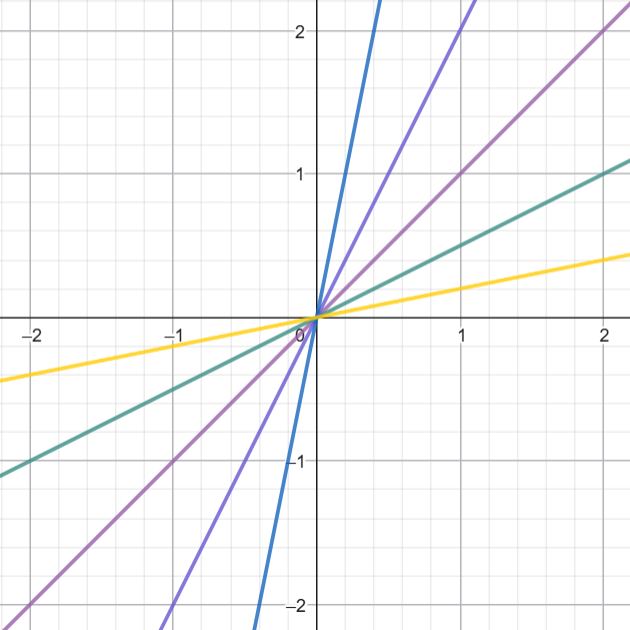
\includegraphics[width=0.86\textwidth]{imagenes/tema2_lineales_1.png}
\end{center}
\begin{itemize}[label=\quad, leftmargin=*, itemsep=0.5em]
  \item[\textcolor{desmosMorado}{$\blacksquare$}] $y=-x$
  \item[\textcolor{desmosAzulFuerte}{$\blacksquare$}] $y=-2x$
  \item[\textcolor{desmosAzul}{$\blacksquare$}] $y=-\dfrac{1}{3}x$
  \item[\textcolor{desmosVerde}{$\blacksquare$}] $y=x+5$
  \item[\textcolor{desmosAmarillo}{$\blacksquare$}] $y=x-3$
\end{itemize}
\begin{center}
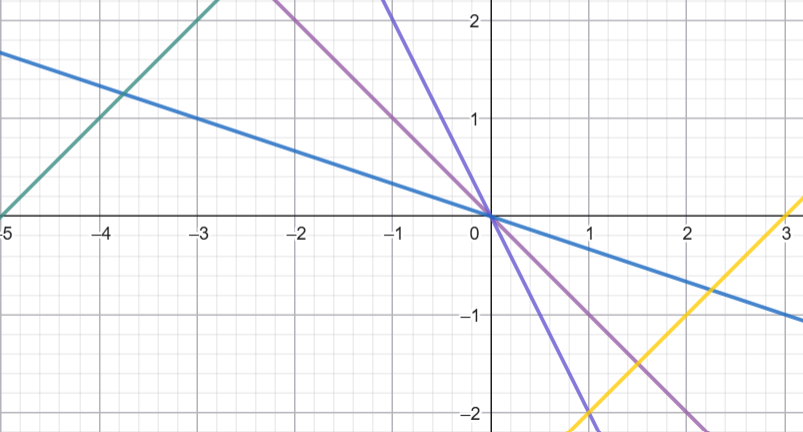
\includegraphics[width=0.86\textwidth]{imagenes/tema2_lineales_2.png}
\end{center}
\begin{itemize}[label=\quad, leftmargin=*, itemsep=0.5em]
  \item[\textcolor{desmosMorado}{$\blacksquare$}] $y=2x+3$
  \item[\textcolor{desmosAzulFuerte}{$\blacksquare$}] $y=2x-3$
  \item[\textcolor{desmosAzul}{$\blacksquare$}] $y=-2x+3$
  \item[\textcolor{desmosVerde}{$\blacksquare$}] $y=-2x-3$
\end{itemize}
\begin{center}
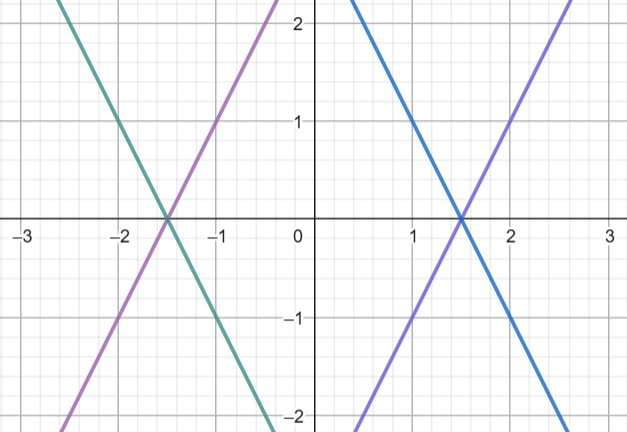
\includegraphics[width=0.86\textwidth]{imagenes/tema2_lineales_3.png}
\end{center}

\subsubsection*{3.- Funciones polinómicas de segundo grado}
\begin{itemize}[label=\quad, leftmargin=*, itemsep=0.5em]
  \item[\textcolor{desmosMorado}{$\blacksquare$}] $y=x^2$
  \item[\textcolor{desmosAzulFuerte}{$\blacksquare$}] $y=2x^2$
  \item[\textcolor{desmosAzul}{$\blacksquare$}] $y=5x^2$
  \item[\textcolor{desmosVerde}{$\blacksquare$}] $y=\dfrac{1}{2}x^2$
  \item[\textcolor{desmosAmarillo}{$\blacksquare$}] $y=-x^2$
\end{itemize}
\begin{center}
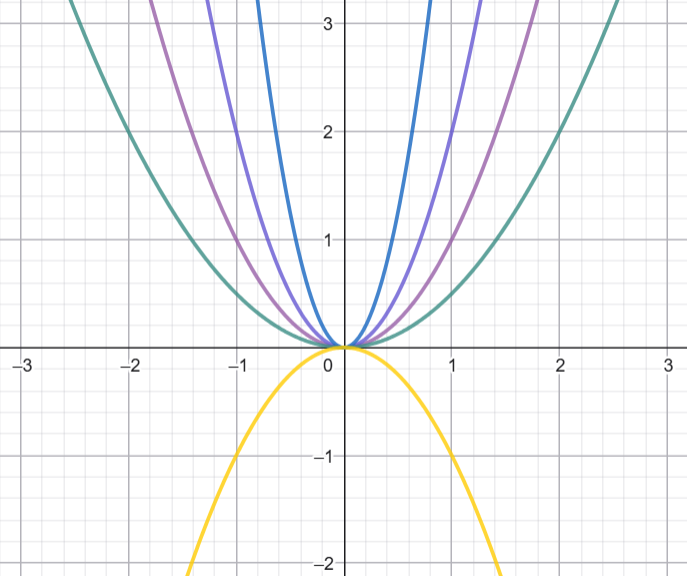
\includegraphics[width=0.86\textwidth]{imagenes/tema2_cuadraticas_1.png}
\end{center}
\begin{itemize}[label=\quad, leftmargin=*, itemsep=0.5em]
  \item[\textcolor{desmosMorado}{$\blacksquare$}] $y=-2x^2$
  \item[\textcolor{desmosAzulFuerte}{$\blacksquare$}] $y=-\dfrac{1}{2}x^2$
  \item[\textcolor{desmosAzul}{$\blacksquare$}] $y=x^2+3$
  \item[\textcolor{desmosVerde}{$\blacksquare$}] $y=x^2-3$
  \item[\textcolor{desmosAmarillo}{$\blacksquare$}] $y=2x^2+1$
\end{itemize}
\begin{center}
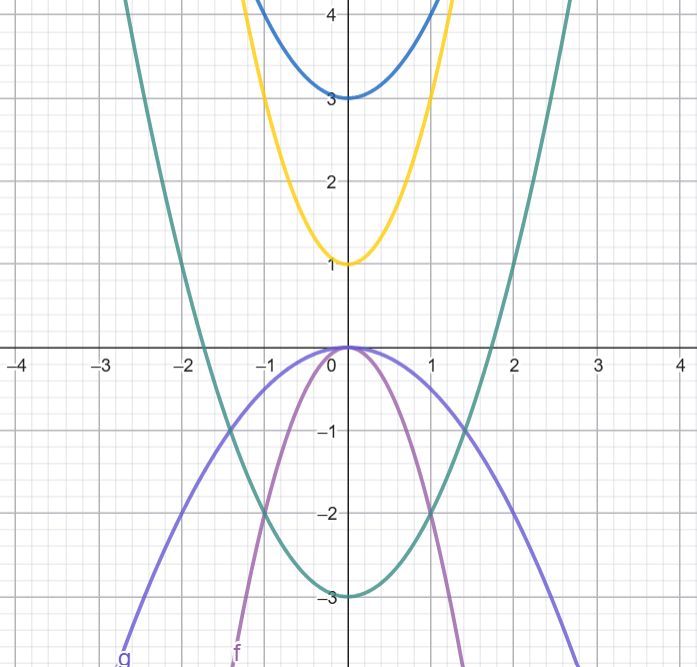
\includegraphics[width=0.86\textwidth]{imagenes/tema2_cuadraticas_2.png}
\end{center}
\begin{itemize}[label=\quad, leftmargin=*, itemsep=0.5em]
  \item[\textcolor{desmosMorado}{$\blacksquare$}] $y=-x^2+2$
  \item[\textcolor{desmosAzulFuerte}{$\blacksquare$}] $y=-x^2-2$
  \item[\textcolor{desmosAzul}{$\blacksquare$}] $y=(x+2)^2$
  \item[\textcolor{desmosVerde}{$\blacksquare$}] $y=(x-3)^2$
  \item[\textcolor{desmosAmarillo}{$\blacksquare$}] $y=(x+2)^2+3$
  \item[\textcolor{desmosMorado}{$\blacksquare$}] $y=(x+2)^2-3$
\end{itemize}
\begin{center}
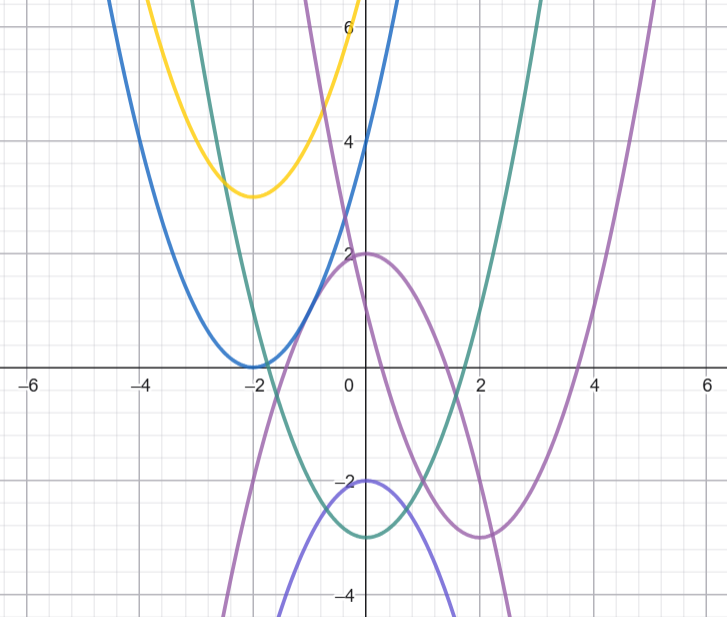
\includegraphics[width=0.86\textwidth]{imagenes/tema2_cuadraticas_3.png}
\end{center}

\subsubsection*{4.- Funciones polinómicas de grado superior a dos}
\begin{itemize}[label=\quad, leftmargin=*, itemsep=0.5em]
  \item[\textcolor{desmosMorado}{$\blacksquare$}] $y=x^3$
  \item[\textcolor{desmosAzulFuerte}{$\blacksquare$}] $y=2x^3$
  \item[\textcolor{desmosAzul}{$\blacksquare$}] $y=-x^3$
  \item[\textcolor{desmosVerde}{$\blacksquare$}] $y=x^3+2$
  \item[\textcolor{desmosAmarillo}{$\blacksquare$}] $y=x^3-2$
\end{itemize}
\begin{center}
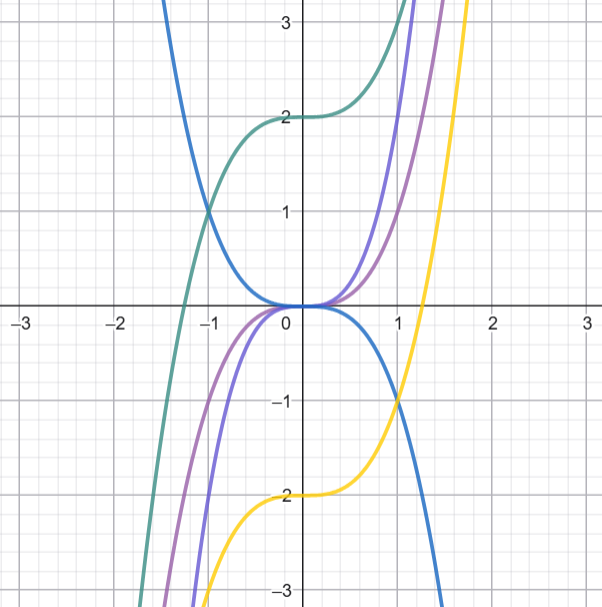
\includegraphics[width=0.86\textwidth]{imagenes/tema2_polinomios_1.png}
\end{center}
\begin{itemize}[label=\quad, leftmargin=*, itemsep=0.5em]
  \item[\textcolor{desmosMorado}{$\blacksquare$}] $y=(x+2)^3$
  \item[\textcolor{desmosAzulFuerte}{$\blacksquare$}] $y=(x-2)^3$
  \item[\textcolor{desmosAzul}{$\blacksquare$}] $y=x^4$
  \item[\textcolor{desmosVerde}{$\blacksquare$}] $y=x^5$
  \item[\textcolor{desmosAmarillo}{$\blacksquare$}] $y=x^6$
\end{itemize}
\begin{center}
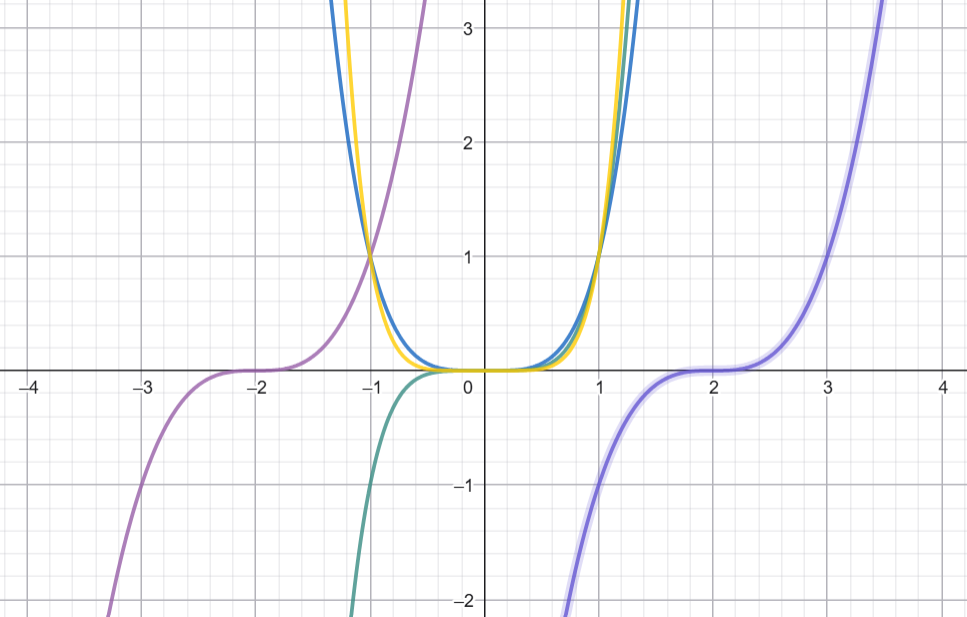
\includegraphics[width=0.86\textwidth]{imagenes/tema2_polinomios_2.png}
\end{center}

\subsubsection*{5.- Funciones racionales}
\begin{itemize}[label=\quad, leftmargin=*, itemsep=0.5em]
  \item[\textcolor{desmosMorado}{$\blacksquare$}] $y=\dfrac{1}{x}$
  \item[\textcolor{desmosAzulFuerte}{$\blacksquare$}] $y=\dfrac{3}{x}$
  \item[\textcolor{desmosAzul}{$\blacksquare$}] $y=\dfrac{7}{x}$
  \item[\textcolor{desmosVerde}{$\blacksquare$}] $y=-\dfrac{1}{x}$
  \item[\textcolor{desmosAmarillo}{$\blacksquare$}] $y=-\dfrac{3}{x}$
\end{itemize}
\begin{center}
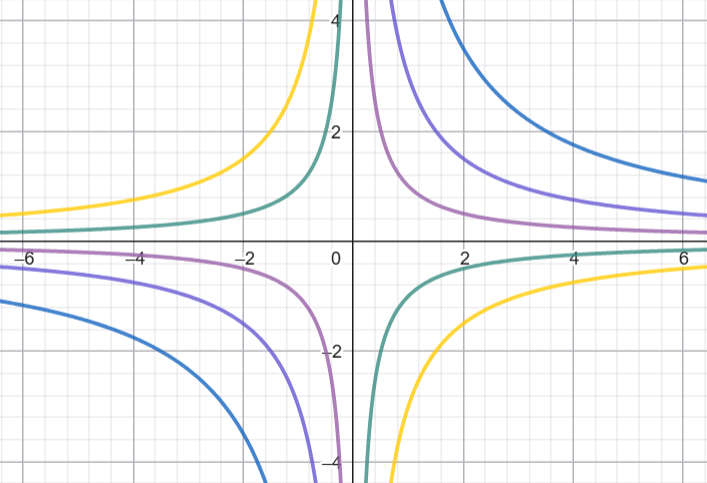
\includegraphics[width=0.86\textwidth]{imagenes/tema2_racionales_1.png}
\end{center}
\begin{itemize}[label=\quad, leftmargin=*, itemsep=0.5em]
  \item[\textcolor{desmosMorado}{$\blacksquare$}] $y=\dfrac{7}{x}+3$
  \item[\textcolor{desmosAzulFuerte}{$\blacksquare$}] $y=\dfrac{7}{x}-2$
  \item[\textcolor{desmosAzul}{$\blacksquare$}] $y=\dfrac{7}{x-2}$
  \item[\textcolor{desmosVerde}{$\blacksquare$}] $y=\dfrac{7}{x+3}$
  \item[\textcolor{desmosAmarillo}{$\blacksquare$}] $y=\dfrac{7}{x+2}-3$
  \item[\textcolor{desmosRojo}{$\blacksquare$}] $y=\dfrac{7}{x+2}+3$
\end{itemize}
\begin{center}
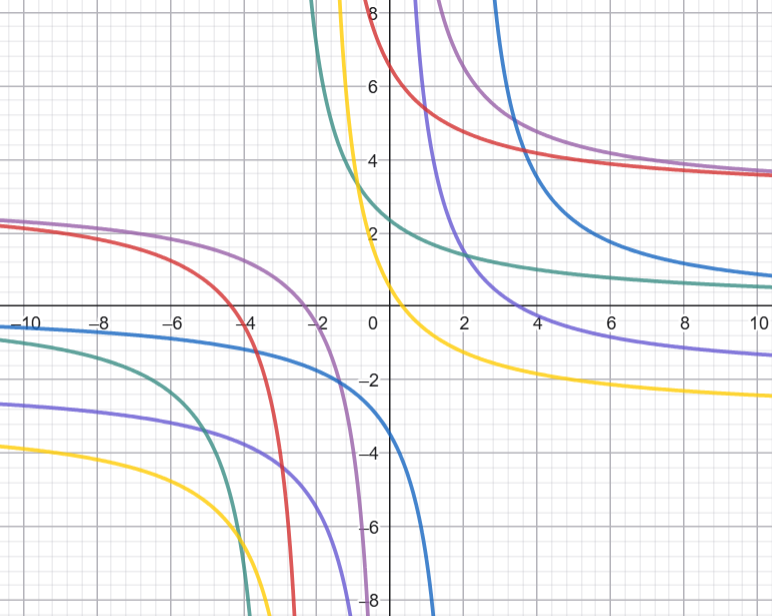
\includegraphics[width=0.86\textwidth]{imagenes/tema2_racionales_2.png}
\end{center}

\subsubsection*{6.- Funciones radicales}
\begin{itemize}[label=\quad, leftmargin=*, itemsep=0.5em]
  \item[\textcolor{desmosMorado}{$\blacksquare$}] $y=\sqrt{x}$
  \item[\textcolor{desmosAzulFuerte}{$\blacksquare$}] $y=-\sqrt{x}$
  \item[\textcolor{desmosAzul}{$\blacksquare$}] $y=\sqrt{x+2}$
  \item[\textcolor{desmosVerde}{$\blacksquare$}] $y=\sqrt{x-3}$
  \item[\textcolor{desmosAmarillo}{$\blacksquare$}] $y=\sqrt{x}+3$
\end{itemize}
\begin{center}
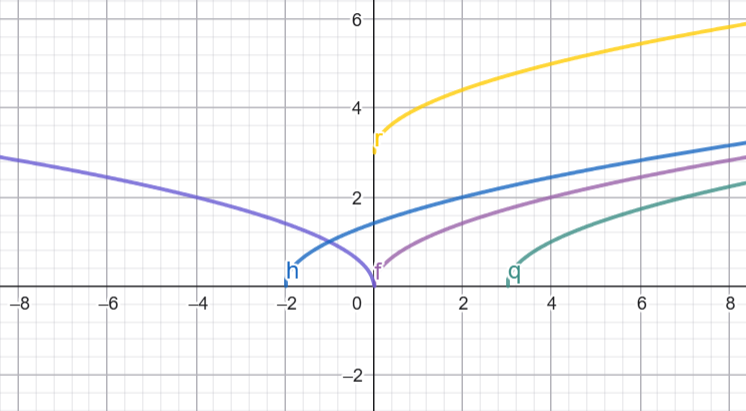
\includegraphics[width=0.86\textwidth]{imagenes/tema2_radicales_1.png}
\end{center}
\begin{itemize}[label=\quad, leftmargin=*, itemsep=0.5em]
  \item[\textcolor{desmosMorado}{$\blacksquare$}] $y=\sqrt{x}-3$
  \item[\textcolor{desmosAzulFuerte}{$\blacksquare$}] $y=\sqrt{x-3}+2$
  \item[\textcolor{desmosAzul}{$\blacksquare$}] $y=\sqrt[3]{x}$
  \item[\textcolor{desmosVerde}{$\blacksquare$}] $y=\sqrt[4]{x}$
\end{itemize}
\begin{center}
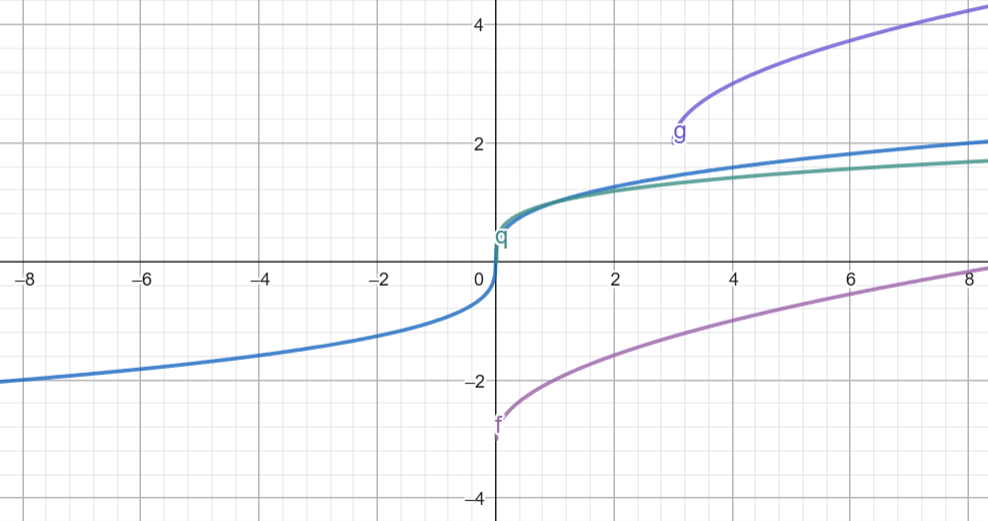
\includegraphics[width=0.86\textwidth]{imagenes/tema2_radicales_2.png}
\end{center}

\subsection*{FUNCIONES TRASCENDENTES}
\subsubsection*{7.- Funciones exponenciales}
\begin{itemize}[label=\quad, leftmargin=*, itemsep=0.5em]
  \item[\textcolor{desmosMorado}{$\blacksquare$}] $y=2^x$
  \item[\textcolor{desmosAzulFuerte}{$\blacksquare$}] $y=2^{-x}$
  \item[\textcolor{desmosAzul}{$\blacksquare$}] $y=\left(\dfrac{1}{2}\right)^x$
  \item[\textcolor{desmosVerde}{$\blacksquare$}] $y=3^x$
  \item[\textcolor{desmosAmarillo}{$\blacksquare$}] $y=2^x+3$
\end{itemize}
\begin{center}
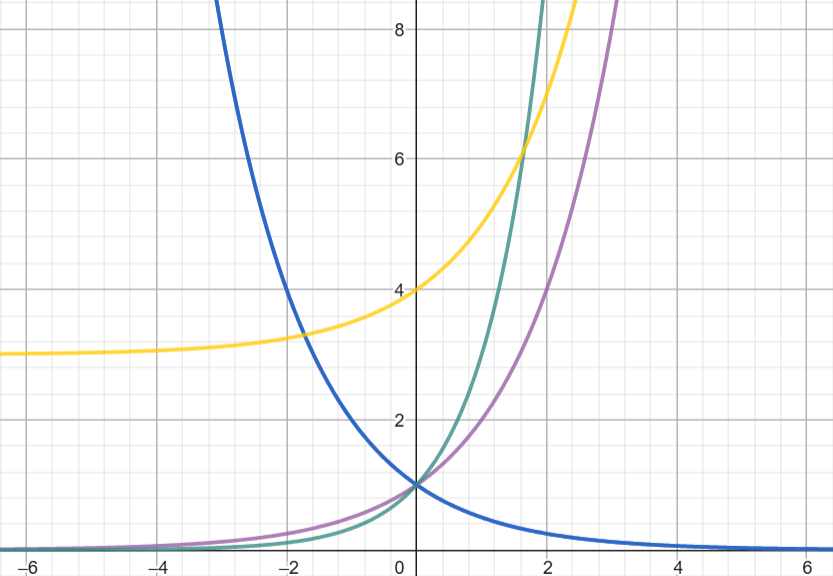
\includegraphics[width=0.86\textwidth]{imagenes/tema2_exponenciales_1.png}
\end{center}
\begin{itemize}[label=\quad, leftmargin=*, itemsep=0.5em]
  \item[\textcolor{desmosMorado}{$\blacksquare$}] $y=2^{x+3}$
  \item[\textcolor{desmosAzulFuerte}{$\blacksquare$}] $y=2^{x-3}-4$
  \item[\textcolor{desmosAzul}{$\blacksquare$}] $y=e^x$
  \item[\textcolor{desmosVerde}{$\blacksquare$}] $y=e^{-x}$
\end{itemize}
\begin{center}
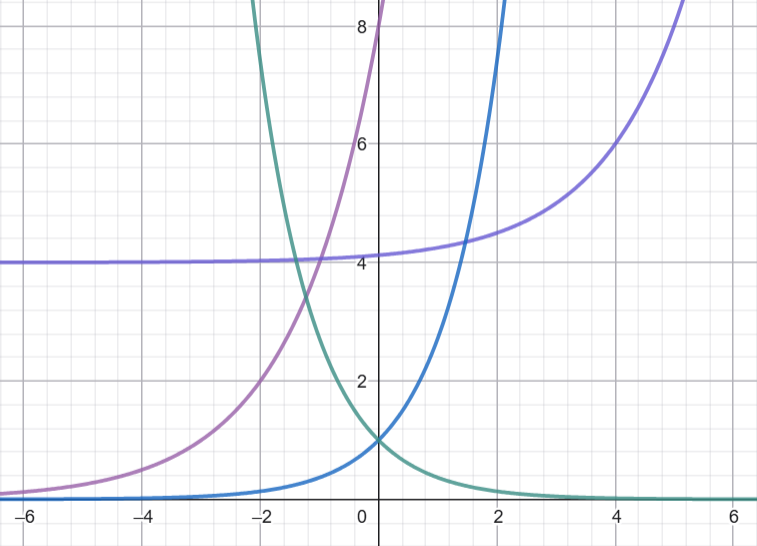
\includegraphics[width=0.86\textwidth]{imagenes/tema2_exponenciales_2.png}
\end{center}

\subsubsection*{8.- Funciones logarítmicas}
\begin{itemize}[label=\quad, leftmargin=*, itemsep=0.5em]
  \item[\textcolor{desmosMorado}{$\blacksquare$}] $y=\log_2 x$
  \item[\textcolor{desmosAzulFuerte}{$\blacksquare$}] $y=\log x$
  \item[\textcolor{desmosAzul}{$\blacksquare$}] $y=\ln x$
  \item[\textcolor{desmosVerde}{$\blacksquare$}] $y=-\log_2 x$
  \item[\textcolor{desmosAmarillo}{$\blacksquare$}] $y=\log_{\dfrac{1}{2}}x$
\end{itemize}
\begin{center}
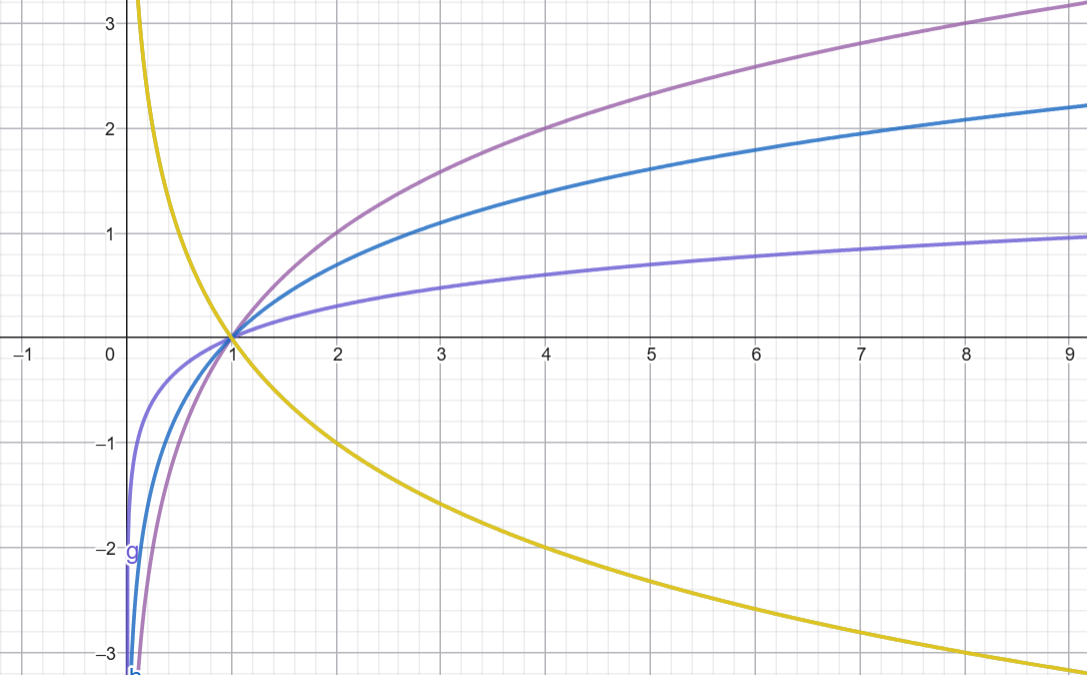
\includegraphics[width=0.86\textwidth]{imagenes/tema2_logaritmicas_1.png}
\end{center}
\begin{itemize}[label=\quad, leftmargin=*, itemsep=0.5em]
  \item[\textcolor{desmosMorado}{$\blacksquare$}] $y=(\log_2 x)+3$
  \item[\textcolor{desmosAzulFuerte}{$\blacksquare$}] $y=\log_2(x+3)$
\end{itemize}
\begin{center}
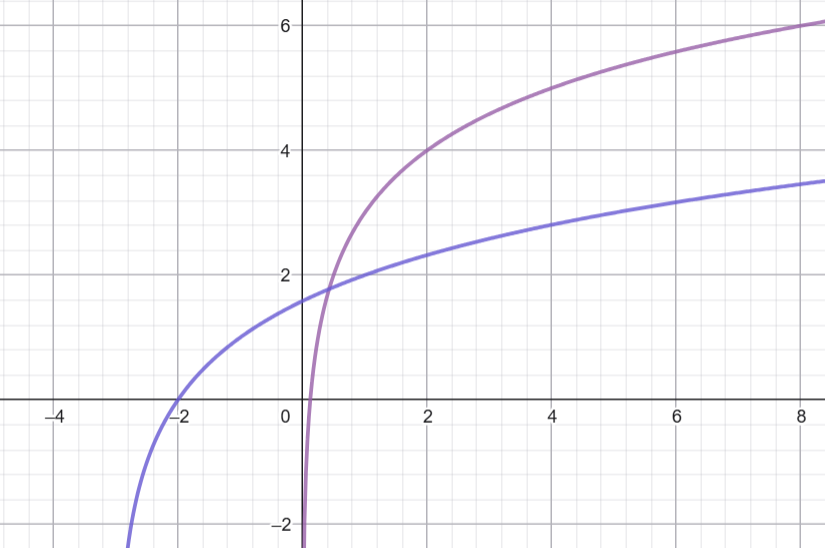
\includegraphics[width=0.86\textwidth]{imagenes/tema2_logaritmicas_2.png}
\end{center}

\subsubsection*{9.- Funciones trigonométricas}
\begin{itemize}[label=\quad, leftmargin=*, itemsep=0.5em]
  \item[\textcolor{desmosMorado}{$\blacksquare$}] $y=\sin x$
  \item[\textcolor{desmosAzulFuerte}{$\blacksquare$}] $y=\cos x$
  \item[\textcolor{desmosAzul}{$\blacksquare$}] $y=\tan x$
  \item[\textcolor{desmosVerde}{$\blacksquare$}] $y=\csc x$
  \item[\textcolor{desmosAmarillo}{$\blacksquare$}] $y=\sec x$
\end{itemize}
\begin{center}
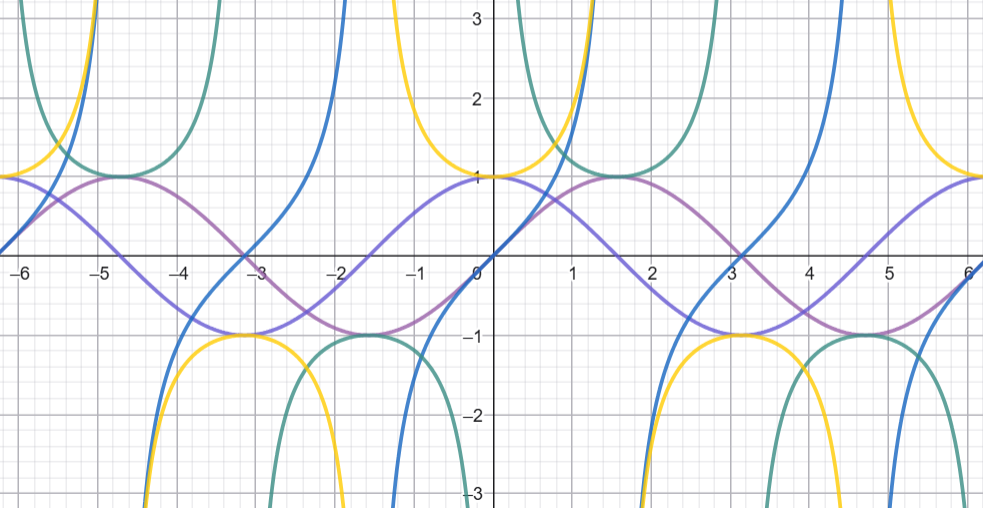
\includegraphics[width=0.86\textwidth]{imagenes/tema2_trigonometricas_1.png}
\end{center}
\begin{itemize}[label=\quad, leftmargin=*, itemsep=0.5em]
  \item[\textcolor{desmosMorado}{$\blacksquare$}] $y=\cot x$
  \item[\textcolor{desmosAzulFuerte}{$\blacksquare$}] $y=2\sin x$
  \item[\textcolor{desmosAzul}{$\blacksquare$}] $y=(\sin x)+2$
  \item[\textcolor{desmosVerde}{$\blacksquare$}] $y=\sin(x+30^\circ)$
\end{itemize}
\begin{center}
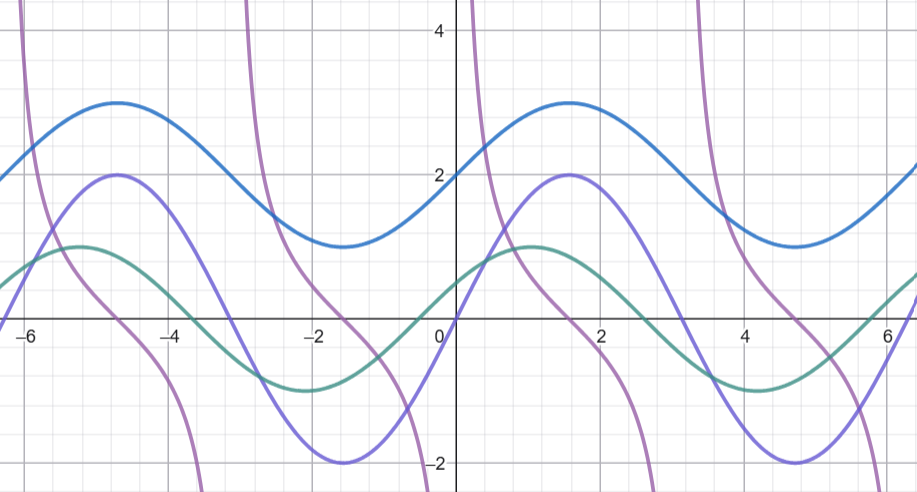
\includegraphics[width=0.86\textwidth]{imagenes/tema2_trigonometricas_2.png}
\end{center}

\subsubsection*{10.- Funciones trigonométricas inversas}
\begin{itemize}[label=\quad, leftmargin=*, itemsep=0.5em]
  \item[\textcolor{desmosMorado}{$\blacksquare$}] $y=\sin^{-1}x$
  \item[\textcolor{desmosAzulFuerte}{$\blacksquare$}] $y=\cos^{-1}x$
  \item[\textcolor{desmosAzul}{$\blacksquare$}] $y=\tan^{-1}x$
  \item[\textcolor{desmosVerde}{$\blacksquare$}] $y=\csc^{-1}x$
  \item[\textcolor{desmosAmarillo}{$\blacksquare$}] $y=\sec^{-1}x$
  \item[\textcolor{desmosRojo}{$\blacksquare$}] $y=\cot^{-1}x$
\end{itemize}
\begin{center}
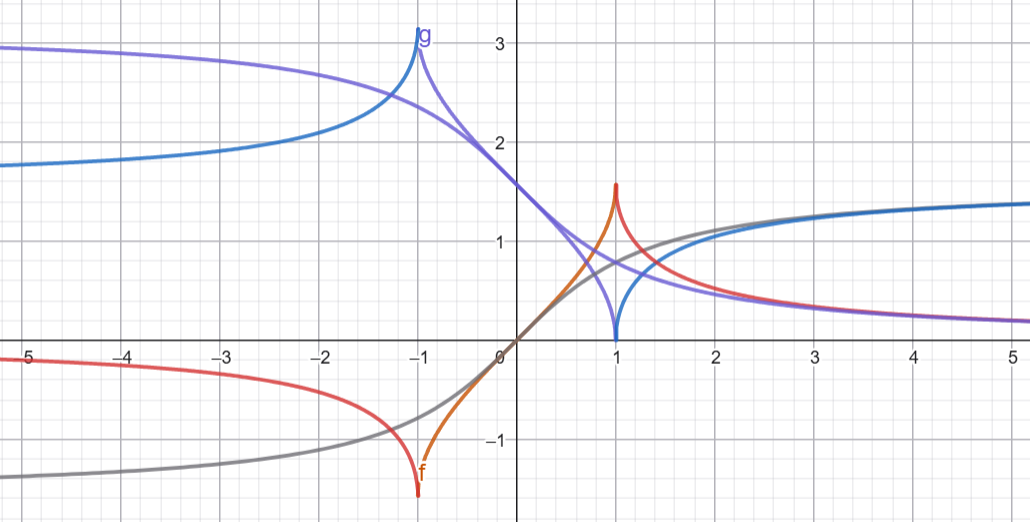
\includegraphics[width=0.86\textwidth]{imagenes/tema2_trigonometricas_inversas.png}
\end{center}

% =================================================
% TEMA 3
% =================================================

\newpage

% Colores de las leyendas de transformaciones
\definecolor{transformNaranja}{HTML}{FF9933}
\definecolor{transformVerdeClaro}{HTML}{CCFF33}
\definecolor{transformVerde}{HTML}{00FF00}
\definecolor{transformCeleste}{HTML}{27F5EB}
\definecolor{transformNegro}{HTML}{000000}
\definecolor{transformGris}{HTML}{CCCCCC}
\definecolor{transformAzul}{HTML}{0000FF}
\definecolor{transformMorado}{HTML}{9900FF}
\definecolor{transformRosa}{HTML}{FF00FF}
\definecolor{transformRojo}{HTML}{FF0000}
\section{Tema 3. Transformación y composición de funciones}

\subsection*{1.- Sea $f(x)=x^2$. Realiza las siguientes transformaciones de la función. Muestra la gráfica resultante.}
\begin{center}
\begin{itemize}[label=\quad, leftmargin=*, itemsep=0.5em]
  \item[\textcolor{transformNaranja}{$\blacksquare$}] Desplazamiento vertical 2 unidades hacia arriba.
  \item[\textcolor{transformVerdeClaro}{$\blacksquare$}] Desplazamiento vertical 2 unidades hacia abajo.
  \item[\textcolor{transformVerde}{$\blacksquare$}] Desplazamiento horizontal 2 unidades a la derecha.
  \item[\textcolor{transformCeleste}{$\blacksquare$}] Desplazamiento horizontal 2 unidades a la izquierda.
  \item[\textcolor{transformNegro}{$\blacksquare$}] Compresión horizontal por un factor de 2.
  \item[\textcolor{transformGris}{$\blacksquare$}] Alargamiento horizontal por un factor de 2.
  \item[\textcolor{transformAzul}{$\blacksquare$}] Alargamiento vertical por un factor de 2.
  \item[\textcolor{transformMorado}{$\blacksquare$}] Compresión vertical por un factor de 2.
  \item[\textcolor{transformRosa}{$\blacksquare$}] Reflexión sobre el eje $x$.
  \item[\textcolor{transformRojo}{$\blacksquare$}] Reflexión sobre el eje $y$.
\end{itemize}
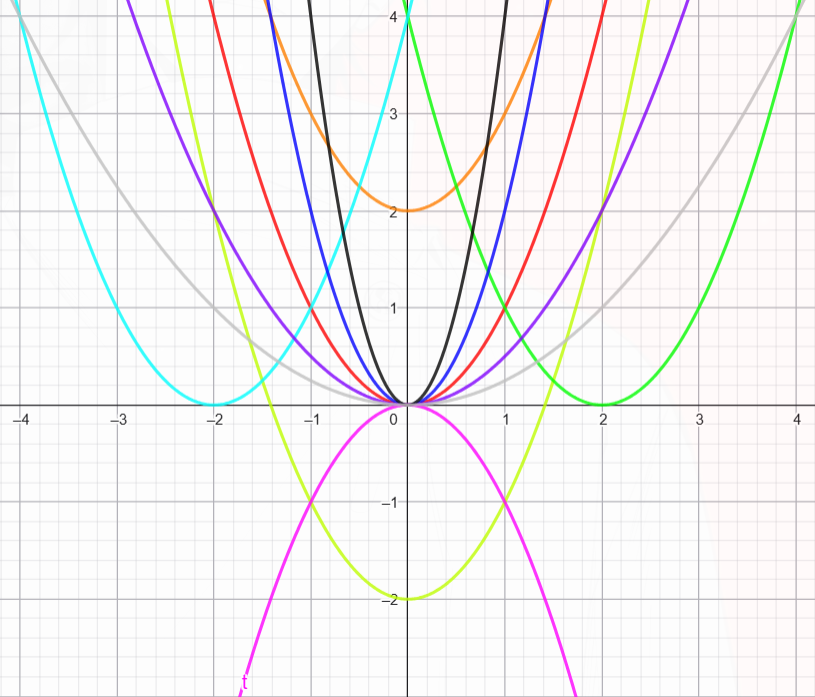
\includegraphics[width=0.86\textwidth]{imagenes/tema3_transformaciones_parabola.png}
\end{center}

\subsection*{2.- Sea $f(x)=\sqrt{x}$. Realiza las siguientes transformaciones de la función. Muestra la gráfica resultante.}
\begin{center}
\begin{itemize}[label=\quad, leftmargin=*, itemsep=0.5em]
  \item[\textcolor{transformNaranja}{$\blacksquare$}] Desplazamiento vertical 2 unidades hacia arriba.
  \item[\textcolor{transformVerdeClaro}{$\blacksquare$}] Desplazamiento vertical 2 unidades hacia abajo.
  \item[\textcolor{transformVerde}{$\blacksquare$}] Desplazamiento horizontal 2 unidades a la derecha.
  \item[\textcolor{transformCeleste}{$\blacksquare$}] Desplazamiento horizontal 2 unidades a la izquierda.
  \item[\textcolor{transformRosa}{$\blacksquare$}] Compresión horizontal por un factor de 2.
  \item[\textcolor{transformNegro}{$\blacksquare$}] Alargamiento horizontal por un factor de 2.
  \item[\textcolor{transformAzul}{$\blacksquare$}] Alargamiento vertical por un factor de 2.
  \item[\textcolor{transformMorado}{$\blacksquare$}] Compresión vertical por un factor de 2.
  \item[\textcolor{transformGris}{$\blacksquare$}] Reflexión sobre el eje $x$.
  \item[\textcolor{transformRojo}{$\blacksquare$}] Reflexión sobre el eje $y$.
\end{itemize}
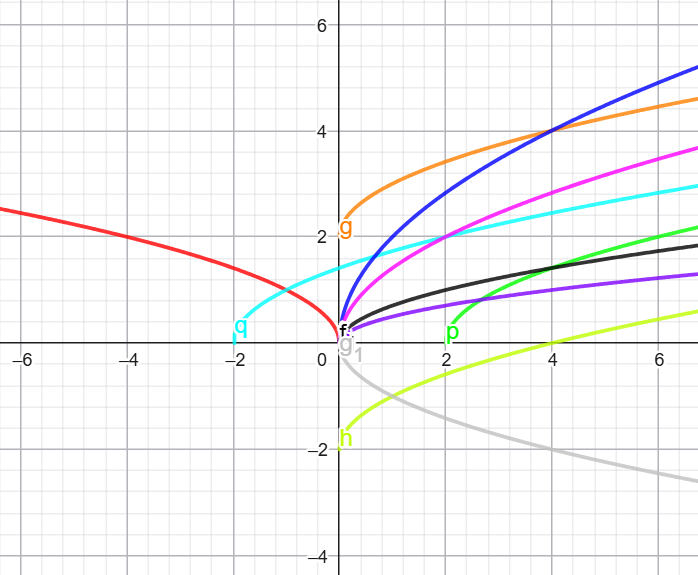
\includegraphics[width=0.86\textwidth]{imagenes/tema3_transformaciones_raiz.png}
\end{center}

\subsection*{3.- Sean $f(x)=\sqrt{x}$, $g(x)=x-3$, $h(x)=\sin x$. Encuentre:}
\begin{enumerate}[label=\alph*)]
  \item $(f\circ g)(x)=f(g(x))=\sqrt{x-3}$, con $x\geq3$.
  \item $(f\circ h)(x)=f(h(x))=\sqrt{\sin x}$, donde $\sin x\geq0$.
  \item $(g\circ f)(x)=g(f(x))=\sqrt{x}-3$, con $x\geq0$.
  \item $(g\circ h)(x)=g(h(x))=\sin x-3$.
  \item $(h\circ f)(x)=h(f(x))=\sin(\sqrt{x})$, con $x\geq0$.
  \item $(h\circ g)(x)=h(g(x))=\sin(x-3)$.
  \item $(f\circ f)(x)=f(f(x))=\sqrt{\sqrt{x}}=\sqrt[4]{x}$, con $x\geq0$.
  \item $(g\circ g)(x)=g(g(x))=(x-3)-3=x-6$.
  \item $(h\circ h)(x)=h(h(x))=\sin(\sin x)$.
\end{enumerate}

% =================================================
% TEMA 4
% =================================================

\newpage
\section{Tema 4. Límites}

\subsection*{1. Grafica la función $f(x)=\dfrac{x^2-1}{x-1}$ e indica cuánto vale $f(1)$. Realiza una conjetura del valor de $\displaystyle\lim_{x\to1}\dfrac{x^2-1}{x-1}$ mediante un tabulado con valores de $x$ cercanos a 1.}
\[
f(x)=\frac{x^2-1}{x-1}=\frac{(x-1)(x+1)}{x-1}=x+1,\qquad x\neq1.
\]
En $x=1$ la expresión original produce $0/0$, por lo que $f(1)$ no está definida. La gráfica es la recta $y=x+1$ con un hueco en $(1,2)$.\begin{center}
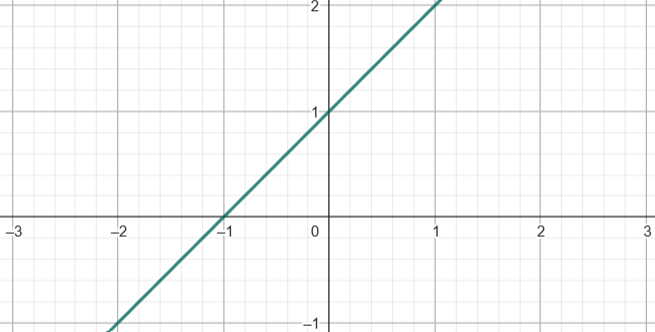
\includegraphics[width=0.86\textwidth]{imagenes/tema4_limites_ejercicio_1.png}
\end{center}
\begin{center}
\begin{tabular}{c|c@{\qquad}c|c}
$x$ (izquierda) & $f(x)$ & $x$ (derecha) & $f(x)$\\\hline
0.9 & 1.9 & 1.1 & 2.1\\
0.99 & 1.99 & 1.01 & 2.01\\
0.999 & 1.999 & 1.001 & 2.001\\
0.9999 & 1.9999 & 1.0001 & 2.0001
\end{tabular}
\end{center}
\respuesta{f(1)\text{ no existe},\qquad \lim_{x\to1}f(x)=2}
\newpage
\subsection*{2. Obtenga la gráfica de la función y a partir de ella indica cuánto vale $f(1)$ y $\displaystyle\lim_{x\to1}f(x)$ para cada uno de los siguientes incisos.}
\begin{enumerate}[label=\alph*)]
  \item $f(x)=\begin{cases}x^2,&x\leq1,\\-x+2,&x>1.\end{cases}$
  \begin{center}
  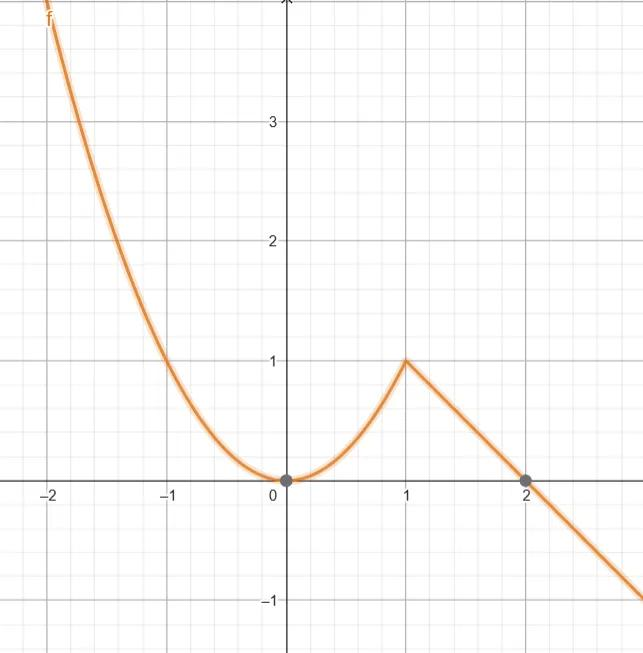
\includegraphics[width=0.86\textwidth]{imagenes/tema4_2_a.jpeg}
  \end{center}
  \[
  f(1)=1^2=1,\qquad
  \lim_{x\to1^-}f(x)=\lim_{x\to1^-}x^2=1^2=1,
  \]
  \[
  \lim_{x\to1^+}f(x)=\lim_{x\to1^+}(-x+2)=-1+2=1.
  \]
  Como los límites laterales coinciden:
  \[
  \boxed{\lim_{x\to1}f(x)=1}.
  \]
  \newpage
  \item $f(x)=\begin{cases}x^2,&x<1,\\-x+2,&x>1.\end{cases}$
  \begin{center}
  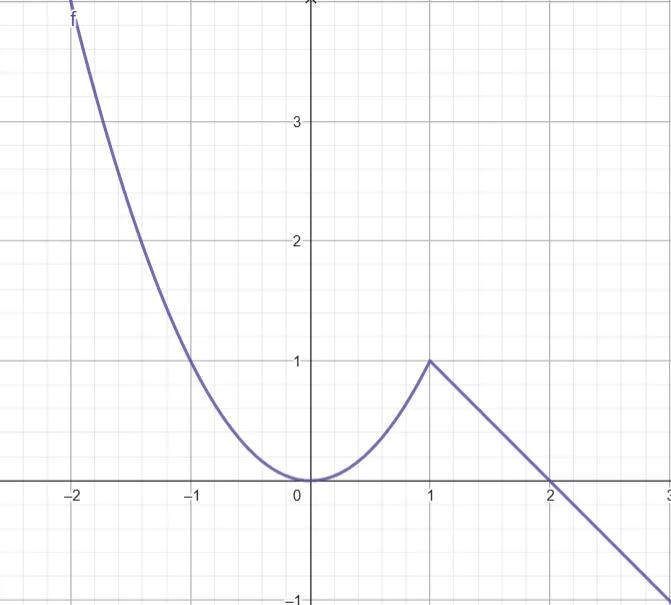
\includegraphics[width=0.86\textwidth]{imagenes/tema4_2_b.jpeg}
  \end{center}
  \[
  f(1)\text{ no está definida},\qquad
  \lim_{x\to1^-}f(x)=\lim_{x\to1^-}x^2=1,
  \]
  \[
  \lim_{x\to1^+}f(x)=\lim_{x\to1^+}(-x+2)=-1+2=1.
  \]
  Por tanto:
  \[
  \boxed{\lim_{x\to1}f(x)=1}.
  \]
  \newpage
  \item $f(x)=\begin{cases}x^2,&x<1,\\3,&x=1,\\-x+2,&x>1.\end{cases}$
  \begin{center}
  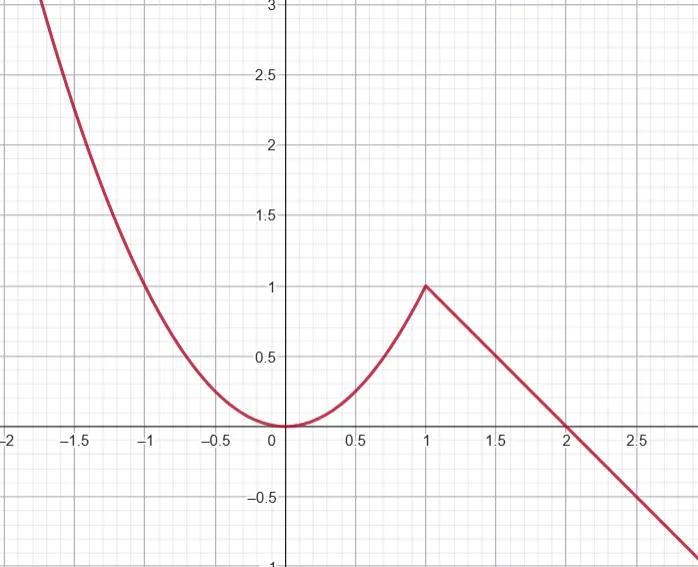
\includegraphics[width=0.86\textwidth]{imagenes/tema4_2_c.jpeg}
  \end{center}
  \[
  f(1)=3,\qquad
  \lim_{x\to1^-}f(x)=\lim_{x\to1^-}x^2=1,
  \]
  \[
  \lim_{x\to1^+}f(x)=\lim_{x\to1^+}(-x+2)=1.
  \]
  El valor puntual no cambia el límite:
  \[
  \boxed{\lim_{x\to1}f(x)=1}.
  \]
  \newpage
  \item $f(x)=\begin{cases}x^2,&x\leq1,\\-x+3,&x>1.\end{cases}$
  \begin{center}
  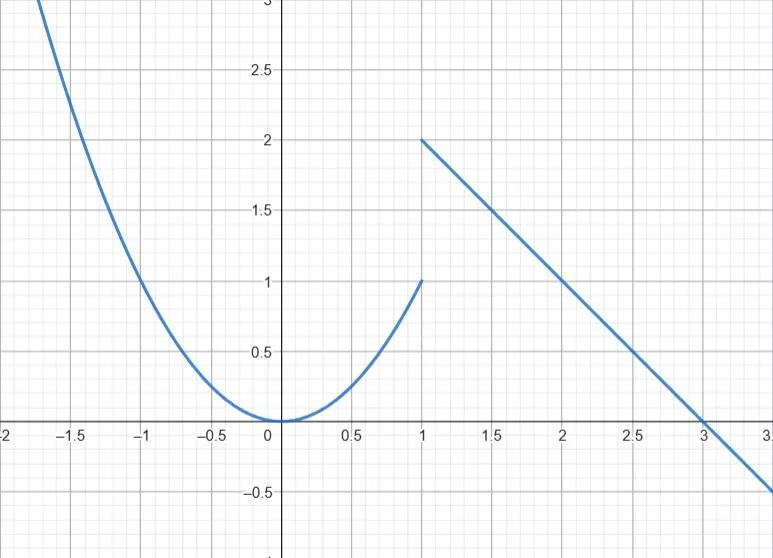
\includegraphics[width=0.86\textwidth]{imagenes/tema4_2_d.jpeg}
  \end{center}
  \[
  f(1)=1^2=1,\qquad
  \lim_{x\to1^-}f(x)=1^2=1,
  \]
  \[
  \lim_{x\to1^+}f(x)=\lim_{x\to1^+}(-x+3)=-1+3=2.
  \]
  Como $1\neq2$:
  \[
  \boxed{\lim_{x\to1}f(x)\text{ no existe}}.
  \]
  \newpage
  \item $f(x)=\begin{cases}x^2,&x<1,\\-x+3,&x>1.\end{cases}$
  \begin{center}
  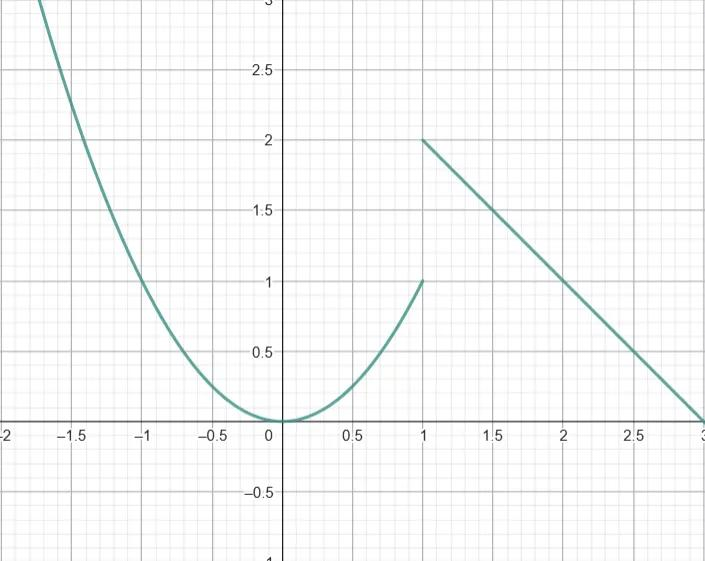
\includegraphics[width=0.86\textwidth]{imagenes/tema4_2_e.jpeg}
  \end{center}
  \[
  f(1)\text{ no está definida},\qquad
  \lim_{x\to1^-}f(x)=1^2=1,
  \]
  \[
  \lim_{x\to1^+}f(x)=\lim_{x\to1^+}(-x+3)=2.
  \]
  Los límites laterales son diferentes:
  \[
  \boxed{\lim_{x\to1}f(x)\text{ no existe}}.
  \]
\end{enumerate}
\newpage
\subsection*{3. Obtenga la gráfica de la función y a partir de ella indica cuánto vale $f(1)$, $\lim_{x\to1^-}f(x)$, $\lim_{x\to1^+}f(x)$ y $\lim_{x\to1}f(x)$ para cada uno de los siguientes incisos.}
\begin{enumerate}[label=\alph*)]
  \item $f(x)=\begin{cases}x^2,&x\leq1,\\-(x-1)^2+1,&x>1.\end{cases}$
  \begin{center}
  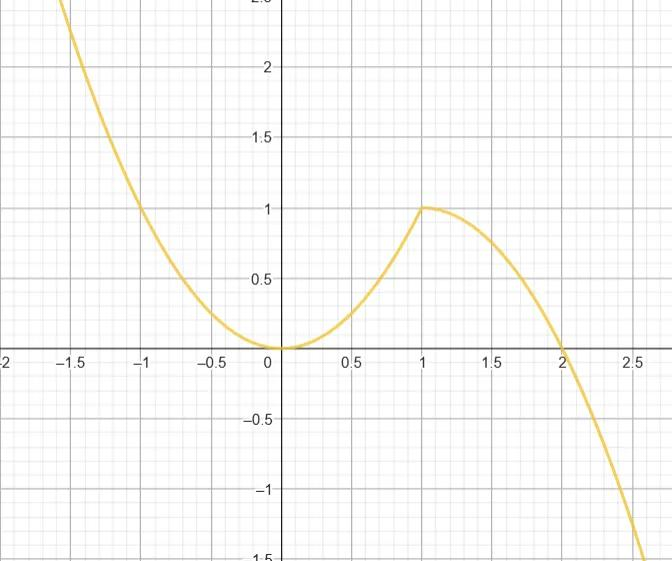
\includegraphics[width=0.86\textwidth]{imagenes/tema4_3_a.jpg}
  \end{center}
  \[
  f(1)=1^2=1,\qquad
  \lim_{x\to1^-}f(x)=1^2=1,
  \]
  \[
  \lim_{x\to1^+}f(x)=-(1-1)^2+1=1.
  \]
  \[
  \boxed{\lim_{x\to1}f(x)=1}.
  \]
  \newpage
  \item $f(x)=\begin{cases}x^2+1,&x\leq1,\\-(x-1)^2+1,&x>1.\end{cases}$
  \begin{center}
  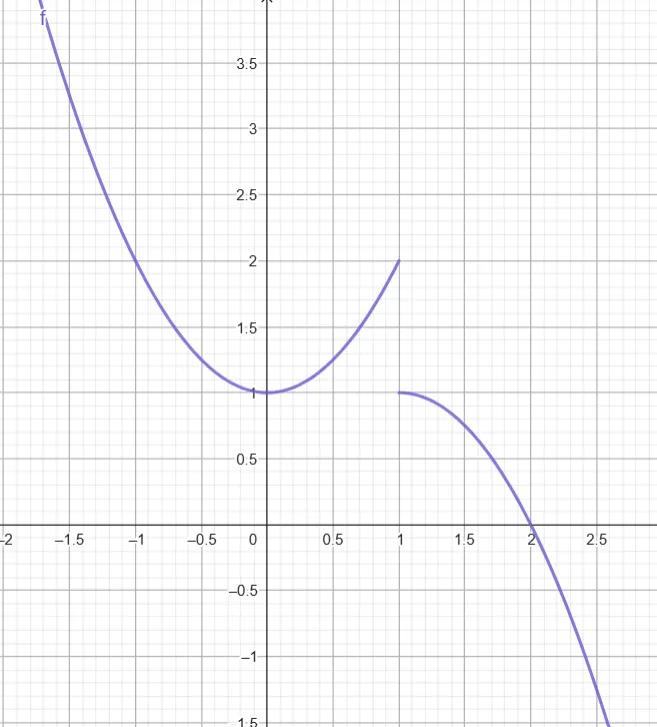
\includegraphics[width=0.86\textwidth]{imagenes/tema4_3_b.jpg}
  \end{center}
  \[
  f(1)=1^2+1=2,\qquad
  \lim_{x\to1^-}f(x)=1^2+1=2,
  \]
  \[
  \lim_{x\to1^+}f(x)=-(1-1)^2+1=1.
  \]
  \[
  2\neq1\quad\Longrightarrow\quad
  \boxed{\lim_{x\to1}f(x)\text{ no existe}}.
  \]
\end{enumerate}

\subsection*{4. Grafica la función $f(x)=\dfrac{1}{|x-1|}$ e indica cuánto vale $f(1)$. Realiza una conjetura del valor de $\displaystyle\lim_{x\to1}\dfrac{1}{|x-1|}$ mediante un tabulado con valores de $x$ cercanos a 1.}
  \begin{center}
  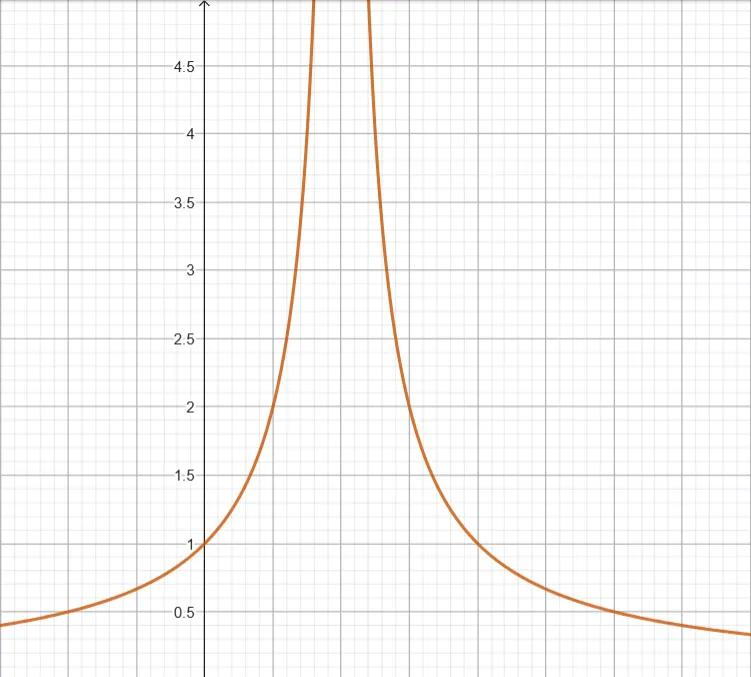
\includegraphics[width=0.86\textwidth]{imagenes/tema4_5.jpg}
  \end{center}
$f(1)$ no está definida porque el denominador vale cero. Al acercarse a 1 por ambos lados, $|x-1|$ se aproxima a cero por valores positivos.
\begin{center}
\begin{tabular}{c|c@{\qquad}c|c}
$x$ (izquierda) & $f(x)$ & $x$ (derecha) & $f(x)$\\\hline
0.9 & 10 & 1.1 & 10\\
0.99 & 100 & 1.01 & 100\\
0.999 & 1000 & 1.001 & 1000
\end{tabular}
\end{center}
\[
\lim_{x\to1^-}|x-1|=0^+,\qquad
\lim_{x\to1^+}|x-1|=0^+,
\]
\[
\frac{1}{|x-1|}\longrightarrow\frac1{0^+}=+\infty.
\]
\respuesta{\lim_{x\to1^-}f(x)=+\infty,\quad \lim_{x\to1^+}f(x)=+\infty,\quad \lim_{x\to1}f(x)=+\infty}

\subsection*{5. Obtenga la gráfica de la función y a partir de ella indica cuánto vale $f(1)$, $\lim_{x\to1^-}f(x)$, $\lim_{x\to1^+}f(x)$ y $\lim_{x\to1}f(x)$ para cada uno de los siguientes incisos.}
\begin{enumerate}[label=\alph*)]
  \item $f(x)=\left(\dfrac{1}{x-1}\right)^2$.
  \begin{center}
  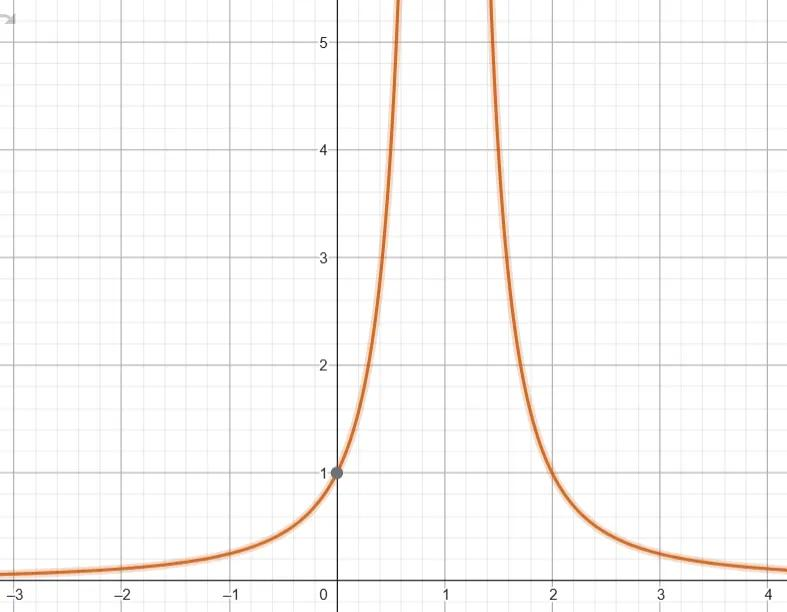
\includegraphics[width=0.86\textwidth]{imagenes/tema4_5_a.jpeg}
  \end{center}
  \[
  x\to1^\pm\Longrightarrow (x-1)^2\to0^+,\qquad
  \left(\frac1{x-1}\right)^2=\frac1{(x-1)^2}\to+\infty.
  \]
  \respuesta{\lim_{x\to1}f(x)=+\infty}
  \newpage
  \item $f(x)=-\left|\dfrac{1}{x-1}\right|$.
  \begin{center}
  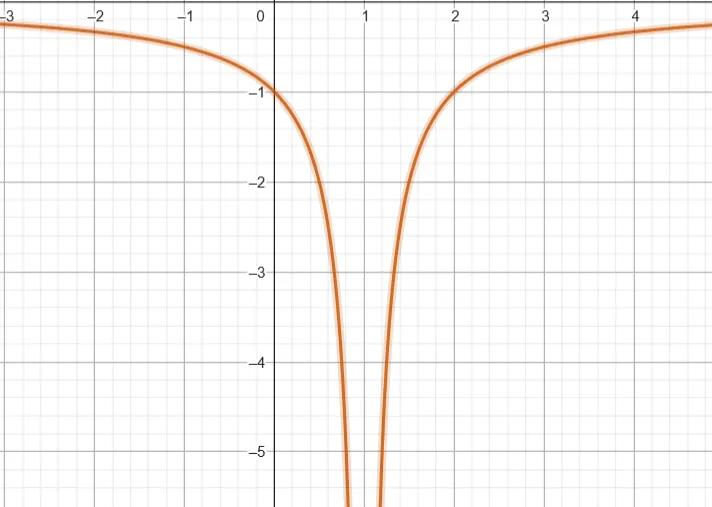
\includegraphics[width=0.86\textwidth]{imagenes/tema4_5_b.jpeg}
  \end{center}
  \[
  \left|\frac1{x-1}\right|=\frac1{|x-1|}\to+\infty,\qquad
  -\left|\frac1{x-1}\right|\to-\infty.
  \]
  \respuesta{\lim_{x\to1}f(x)=-\infty}
  \newpage
  \item $f(x)=\dfrac{1}{x-1}$.
  \begin{center}
  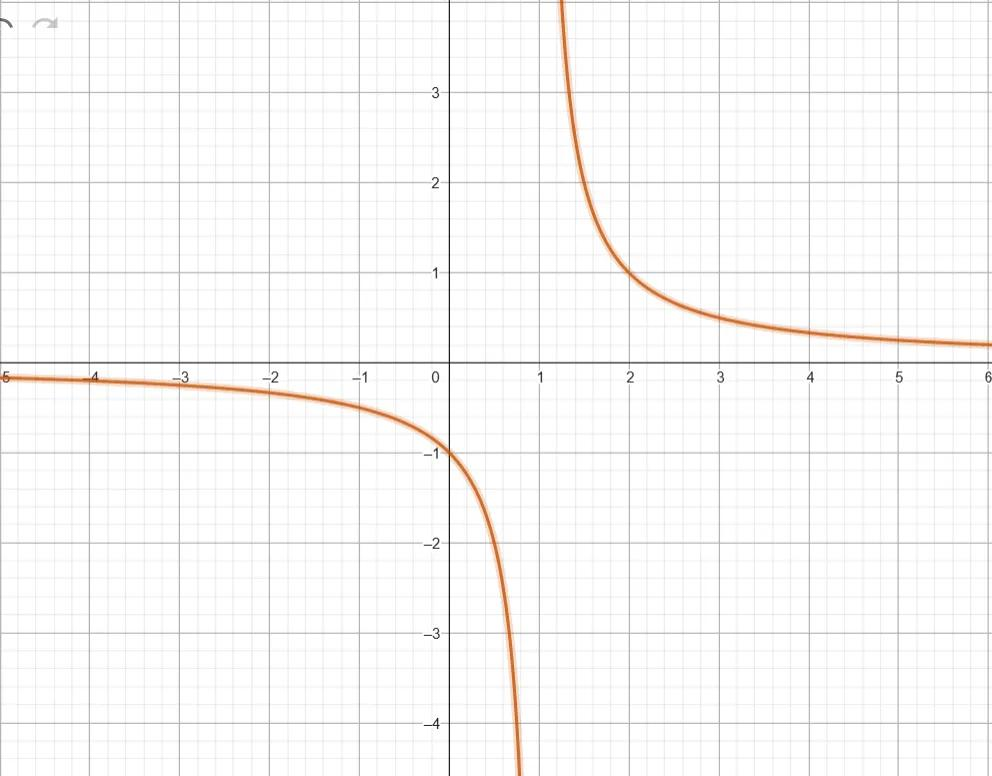
\includegraphics[width=0.86\textwidth]{imagenes/tema4_5_c.jpeg}
  \end{center}
  \[
  x\to1^-:\ x-1\to0^-\Rightarrow\frac1{x-1}\to-\infty,
  \qquad
  x\to1^+:\ x-1\to0^+\Rightarrow\frac1{x-1}\to+\infty.
  \]
  \respuesta{\lim_{x\to1}f(x)\text{ no existe}}
  \newpage
  \item $f(x)=-\dfrac{1}{x-1}$.
  \begin{center}
  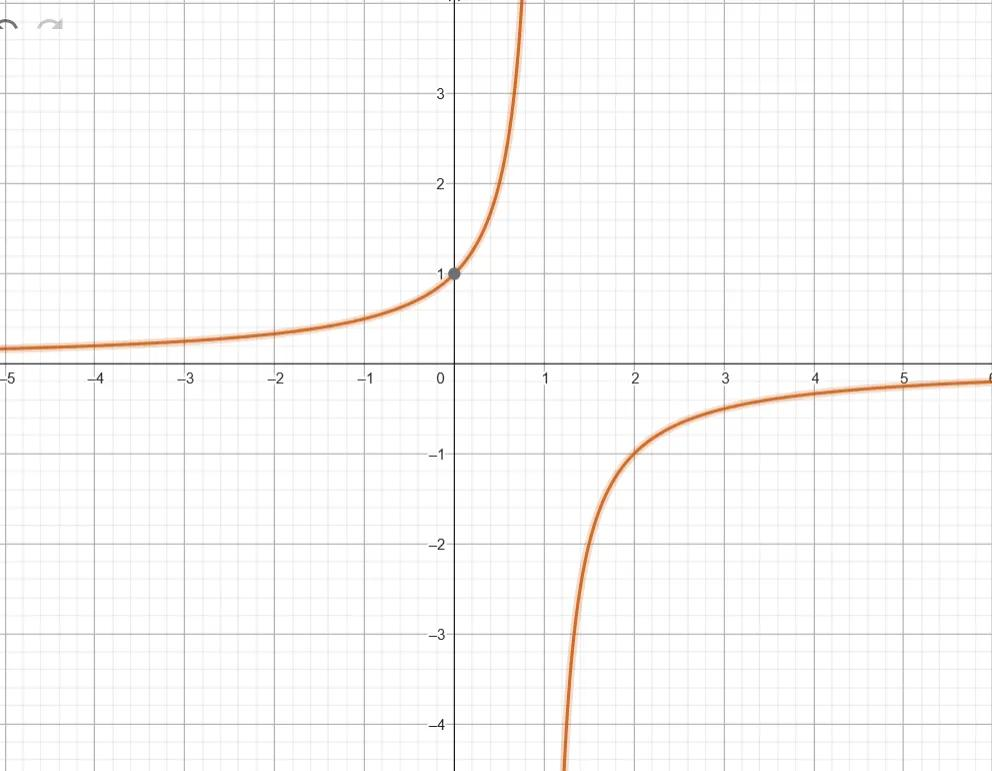
\includegraphics[width=0.86\textwidth]{imagenes/tema4_5_d.jpeg}
  \end{center}
  \[
  x\to1^-:\ -\frac1{x-1}\to+\infty,\qquad
  x\to1^+:\ -\frac1{x-1}\to-\infty.
  \]
  \respuesta{\lim_{x\to1}f(x)\text{ no existe}}
\end{enumerate}

\subsection*{6. Evalúe los siguientes límites eliminando las indeterminaciones por métodos algebraicos.}
\textbf{Procedimiento general:} primero se sustituye el valor al que tiende $x$. Si se obtiene una indeterminación del tipo $\frac00$, se factoriza o racionaliza para cancelar el factor que provoca la indeterminación. No se cancela cualquier expresión que aún dependa de $x$ sin comprobar que se mantiene válida para $x\neq a$.
\begin{enumerate}[label=\alph*)]
  \item $\displaystyle\lim_{x\to0}\frac{x^2}{x}$. Al sustituir se obtiene $\frac00$. Como $x\neq0$ cerca del punto,
  \[
  \frac{x^2}{x}=x.
  \]
  Por tanto,
  \[
  \lim_{x\to0}\frac{x^2}{x}
  =\lim_{x\to0}\frac{x\cdot x}{x}
  =\lim_{x\to0}x
  =\boxed{0}.
  \]
  \item $\displaystyle\lim_{x\to5}\frac{x^2-6x+5}{x-5}$. Primero factorizamos el numerador:
  \[
  x^2-6x+5=(x-1)(x-5).
  \]
  Luego cancelamos el factor común $(x-5)$, válido para $x\neq5$:
  \[
  \lim_{x\to5}\frac{x^2-6x+5}{x-5}
  =\lim_{x\to5}\frac{(x-1)(x-5)}{x-5}
  =\lim_{x\to5}(x-1)
  =5-1=\boxed{4}.
  \]
  \item $\displaystyle\lim_{x\to4}\frac{x^2-4x}{x^2-3x-4}$. Al sustituir se obtiene $\frac00$. Factorizamos:
  \[
  x^2-4x=x(x-4),
  \qquad
  x^2-3x-4=(x-4)(x+1).
  \]
  Cancelando $(x-4)$:
  \[
  \lim_{x\to4}\frac{x^2-4x}{x^2-3x-4}
  =\lim_{x\to4}\frac{x(x-4)}{(x-4)(x+1)}
  =\lim_{x\to4}\frac{x}{x+1}
  =\frac45.
  \]
  \item $\displaystyle\lim_{x\to-3}\frac{x^2-9}{2x^2+7x+3}$. Al sustituir se obtiene $\frac00$. Factorizamos ambos polinomios:
  \[
  x^2-9=(x-3)(x+3),
  \qquad
  2x^2+7x+3=(2x+1)(x+3).
  \]
  Después de cancelar $(x+3)$:
  \[
  \lim_{x\to-3}\frac{x^2-9}{2x^2+7x+3}
  =\lim_{x\to-3}\frac{(x-3)(x+3)}{(2x+1)(x+3)}
  =\lim_{x\to-3}\frac{x-3}{2x+1}
  =\frac{-6}{-5}=\boxed{\frac65}.
  \]
  \item $\displaystyle\lim_{x\to-2}\frac{x+2}{x^3+8}$. La suma de cubos factoriza como
  \[
  x^3+8=(x+2)(x^2-2x+4).
  \]
  \[
  \lim_{x\to-2}\frac{x+2}{x^3+8}
  =\lim_{x\to-2}\frac{x+2}{(x+2)(x^2-2x+4)}
  =\lim_{x\to-2}\frac1{x^2-2x+4}
  =\frac1{4+4+4}=\boxed{\frac1{12}}.
  \]
  \item $\displaystyle\lim_{x\to1}\frac{x^4-1}{x^3-1}$. Aplicamos diferencia de cuadrados y diferencia de cubos:
  \[
  x^4-1=(x-1)(x+1)(x^2+1),
  \qquad
  x^3-1=(x-1)(x^2+x+1).
  \]
  \[
  \lim_{x\to1}\frac{x^4-1}{x^3-1}
  =\lim_{x\to1}\frac{(x+1)(x^2+1)}{x^2+x+1}
  =\frac{2(2)}3=\boxed{\frac43}.
  \]
  \item $\displaystyle\lim_{x\to-1}\frac{x^2+2x+1}{x^4-1}$. Factorizamos un trinomio cuadrado perfecto y una diferencia de cuadrados:
  \[
  x^2+2x+1=(x+1)^2,
  \qquad
  x^4-1=(x-1)(x+1)(x^2+1).
  \]
  Cancelamos un factor $(x+1)$ y sustituimos:
  \[
  \lim_{x\to-1}\frac{(x+1)^2}{(x-1)(x+1)(x^2+1)}
  =\lim_{x\to-1}\frac{x+1}{(x-1)(x^2+1)}
  =\boxed{0}.
  \]
  \item $\displaystyle
  \lim_{x\to0}\frac{\sqrt{9+x}-3}{x}
  =\lim_{x\to0}\frac{(\sqrt{9+x}-3)(\sqrt{9+x}+3)}
  {x(\sqrt{9+x}+3)}
  =\lim_{x\to0}\frac{x}{x(\sqrt{9+x}+3)}
  =\frac1{3+3}=\boxed{\frac16}$.
  \item $\displaystyle
  \lim_{x\to3}\frac{\sqrt{x+1}-2}{x-3}
  =\lim_{x\to3}\frac{x+1-4}{(x-3)(\sqrt{x+1}+2)}
  =\lim_{x\to3}\frac1{\sqrt{x+1}+2}
  =\frac14=\boxed{\frac14}$.
  \item $\displaystyle
  \lim_{x\to-4}\frac{\sqrt{x^2+9}-5}{x+4}
  =\lim_{x\to-4}\frac{x^2+9-25}
  {(x+4)(\sqrt{x^2+9}+5)}
  =\lim_{x\to-4}\frac{x-4}{\sqrt{x^2+9}+5}
  =\frac{-8}{10}=\boxed{-\frac45}$.
\end{enumerate}

% =================================================
% TEMA 5
% =================================================

\newpage
\section{Tema 5. Continuidad}

\subsection*{1.- En cada uno de los siguientes ejercicios, determina si la función es continua en $x=a$. Justifica claramente tu respuesta a partir de la definición de continuidad.}
Para que $f$ sea continua en $x=a$ deben cumplirse simultáneamente: (1) $f(a)$ está definida; (2) existe $\lim_{x\to a}f(x)$; y (3) el límite es igual a $f(a)$.
\begin{enumerate}[label=\alph*)]
  \item $f(x)=\dfrac{1}{x-3},\ a=3$. $f(3)$ no está definida y el límite bilateral no existe (los laterales divergen con signos opuestos). \textbf{No es continua} en $x=3$.
  \item $f(x)=\dfrac{x^2-9}{x-3},\ a=3$. Para $x\neq3$, $f(x)=x+3$, por lo que $\lim_{x\to3}f(x)=6$. Sin embargo, $f(3)$ no está definida. \textbf{No es continua} en $x=3$.
  \item $f(x)=\begin{cases}\dfrac{1}{x-3},&x\neq3,\\2,&x=3.\end{cases},\ a=3$. $f(3)=2$, pero $\lim_{x\to3^-}f(x)=-\infty$ y $\lim_{x\to3^+}f(x)=+\infty$. El límite bilateral no existe. \textbf{No es continua}.
  \item $f(x)=\begin{cases}\dfrac{x^2-9}{x-3},&x\neq3,\\2,&x=3.\end{cases},\ a=3$. Para $x\neq3$, $f(x)=x+3$, así que $\lim_{x\to3}f(x)=6$, mientras que $f(3)=2$. Como $6\neq2$, \textbf{no es continua}.
  \item $f(x)=\begin{cases}\dfrac{x^2-9}{x-3},&x\neq3,\\6,&x=3.\end{cases},\ a=3$. Para $x\neq3$, $f(x)=x+3$; por tanto, $\lim_{x\to3}f(x)=6=f(3)$. Se cumplen las tres condiciones: \textbf{sí es continua} en $x=3$.
\end{enumerate}

\subsection*{2.- Grafica la siguiente función seccionada. Identifica todos los valores de $x$ en los que la función no es continua. Para cada uno de dichos valores, determina: a) si la función es continua por la izquierda, b) si la función es continua por la derecha. Establezca todos los intervalos sobre los que la función es continua.}
\[
f(x)=\begin{cases}
-x,&x\leq-4,\\
x,&-4<x\leq-2,\\
x^2,&-2<x<2,\\
-2,&x=2,\\
x-3,&x>2.
\end{cases}
\]
  \begin{center}
  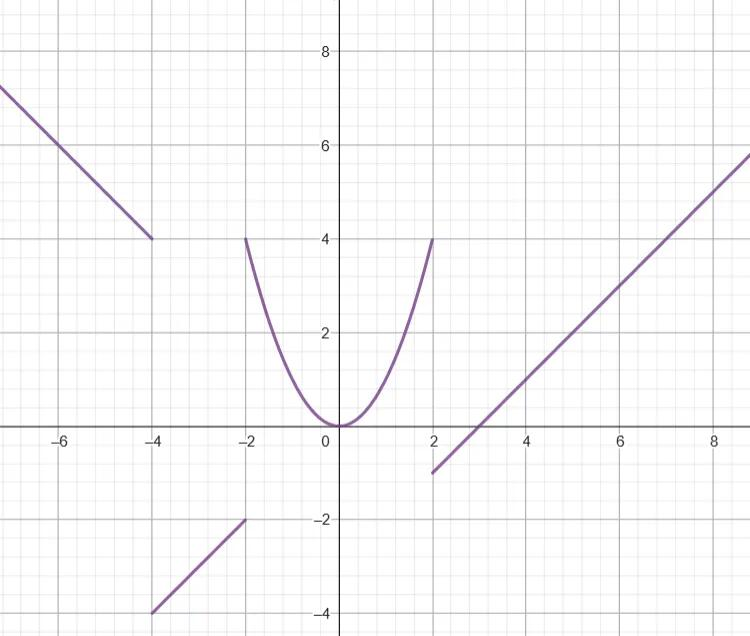
\includegraphics[width=0.86\textwidth]{imagenes/tema5_2.jpeg}
  \end{center}
Los posibles puntos de discontinuidad son los cambios de regla: $x=-4,-2,2$.
\begin{itemize}
  \item En $x=-4$: $f(-4)=4$ y $\lim_{x\to-4^-}f(x)=4$, pero $\lim_{x\to-4^+}f(x)=-4$. Es \textbf{continua por la izquierda}, no por la derecha.
  \item En $x=-2$: $f(-2)=-2$ y $\lim_{x\to-2^-}f(x)=-2$, mientras que $\lim_{x\to-2^+}f(x)=4$. Es \textbf{continua por la izquierda}, no por la derecha.
  \item En $x=2$: $f(2)=-2$, $\lim_{x\to2^-}f(x)=4$ y $\lim_{x\to2^+}f(x)=-1$. No es continua ni por la izquierda ni por la derecha.
\end{itemize}
Los intervalos máximos en los que es continua son:
\[
\boxed{(-\infty,-4],\quad(-4,-2],\quad(-2,2),\quad(2,+\infty).}
\]
\newpage
\subsection*{3.- Sea la función seccionada:}
\[
f(x)=\begin{cases}
x^2,&0\leq x\leq2,\\
x,&2<x<4,\\
4,&4<x\leq6.
\end{cases}
\]
Para cada una de las siguientes afirmaciones responde Falso (F) o Verdadero (V). En caso de ser falso explica por qué.
\begin{enumerate}[label=\alph*)]
  \item $f(2)=4$. \textbf{V}.
  \item $\lim_{x\to2^-}f(x)=4$. \textbf{V}, porque por la izquierda se usa $x^2$.
  \item $\lim_{x\to2^+}f(x)=2$. \textbf{V}, porque por la derecha se usa $x$.
  \item $\lim_{x\to2}f(x)$ no está definido. \textbf{V}, los límites laterales son distintos ($4\neq2$).
  \item $f(x)$ es continua por la izquierda en $x=2$. \textbf{V}, $\lim_{x\to2^-}f(x)=f(2)=4$.
  \item $f(x)$ es continua por la derecha en $x=2$. \textbf{F}, pues $\lim_{x\to2^+}f(x)=2\neq f(2)=4$.
  \item $f(x)$ es continua en $x=2$. \textbf{F}, el límite bilateral no existe.
  \item $f(x)$ es continua en el intervalo $[0,2]$. \textbf{V}, en ese intervalo coincide con $x^2$.
  \item $f(4)$ no está definida. \textbf{V}, ninguno de los tramos incluye $x=4$.
  \item $\lim_{x\to4^-}f(x)=2$. \textbf{F}, el límite por la izquierda es $4$.
  \item $\lim_{x\to4^+}f(x)=4$. \textbf{V}, a la derecha la función vale constantemente $4$.
  \item $\lim_{x\to4}f(x)=4$. \textbf{V}, ambos límites laterales valen $4$, aunque $f(4)$ no esté definida.
  \item $f(x)$ es continua por la izquierda en $x=4$. \textbf{F}, porque $f(4)$ no existe.
  \item $f(x)$ es continua por la derecha en $x=4$. \textbf{F}, porque $f(4)$ no existe.
  \item $f(x)$ es continua en $x=4$. \textbf{F}, no está definida en ese punto.
  \item $f(x)$ es continua en el intervalo $[2,4]$. \textbf{F}, $f(4)$ no está definida y además hay una discontinuidad en $x=2$.
  \item $f(x)$ es continua en el intervalo $(2,4)$. \textbf{V}, en ese intervalo $f(x)=x$.
\end{enumerate}

% =================================================
% TEMA 6
% =================================================

\newpage
\section{Tema 6. Límites cuando $x$ tiende a infinito}

\subsection*{1.- Para las siguientes funciones, realiza una conjetura del valor de $\lim_{x\to\infty}f(x)$ y de $\lim_{x\to-\infty}f(x)$ mediante un tabulado.}
\begin{enumerate}[label=\alph*)]
  \item $f(x)=\dfrac{2x+1}{x-2}$. Dividiendo entre $x$: $f(x)=\dfrac{2+1/x}{1-2/x}$. En ambos extremos se aproxima a $2$.\\
  \respuesta{\lim_{x\to+\infty}f(x)=2,\qquad\lim_{x\to-\infty}f(x)=2}
  \item $f(x)=\sqrt{x^2}=|x|$.\\
  \respuesta{\lim_{x\to+\infty}f(x)=+\infty,\qquad\lim_{x\to-\infty}f(x)=+\infty}
  \item $f(x)=-\dfrac{x^3}{4}$.\\
  \respuesta{\lim_{x\to+\infty}f(x)=-\infty,\qquad\lim_{x\to-\infty}f(x)=+\infty}
\end{enumerate}
\textbf{Tabulado para observar el comportamiento en ambos extremos:}
\begin{center}
\begin{tabular}{r|r|r|r}
$x$ & $f_a(x)=\frac{2x+1}{x-2}$ & $f_b(x)=\sqrt{x^2}$ & $f_c(x)=-\frac{x^3}{4}$\\\hline
$-100$ & $1.9510$ & $100$ & $250000$\\
$-10$ & $1.5833$ & $10$ & $2500$\\
$10$ & $2.6250$ & $10$ & $-2500$\\
$100$ & $2.0510$ & $100$ & $-250000$
\end{tabular}
\end{center}
\newpage
\subsection*{2.- Evaluar los siguientes límites mediante manipulaciones algebraicas. Agrega la gráfica de la función y traza la asíntota horizontal correspondiente (si existe) para verificar tu respuesta.}
\textbf{Criterio práctico:} para cocientes de polinomios se divide numerador y denominador entre la máxima potencia de $x$. Si los grados son iguales, el límite es el cociente de los coeficientes principales; si el grado del denominador es mayor, el límite es $0$; si el grado del numerador es mayor, el límite será $+\infty$ o $-\infty$ según los signos.
\begin{enumerate}[label=\alph*)]
  \item $\displaystyle\lim_{x\to\infty}\frac{x^3+2x}{x^2-1}$. Dividimos entre $x^2$:
  \[
  \frac{x^3+2x}{x^2-1}
  =\frac{x+\frac{2}{x}}{1-\frac1{x^2}}.
  \]
  Como $\frac2x\to0$ y $\frac1{x^2}\to0$, pero $x\to+\infty$:
  \[
  \lim_{x\to\infty}\frac{x+2/x}{1-1/x^2}=+\infty.
  \]
  No existe asíntota horizontal.
  \begin{center}
  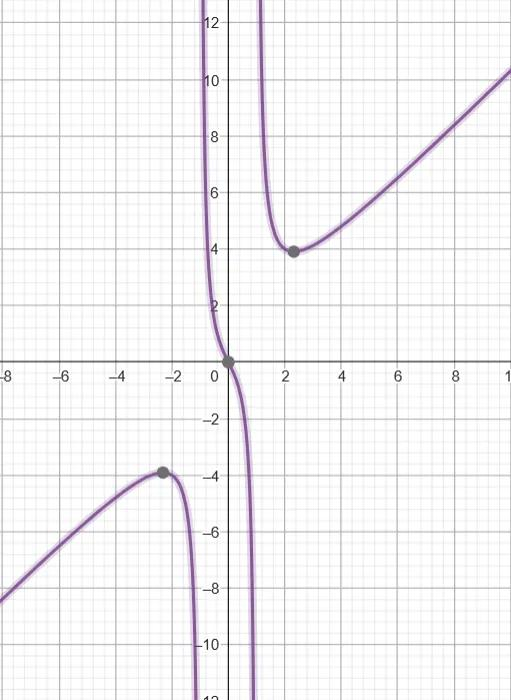
\includegraphics[width=0.65\textwidth]{imagenes/tema6_2_a.jpeg}
  \end{center}
  \newpage
  \item $\displaystyle\lim_{x\to-\infty}\frac{x^3+2x}{x^2-1}$. Dividimos numerador y denominador entre $x^2$:
  \[
  \frac{x^3+2x}{x^2-1}
  =\frac{x+\frac2x}{1-\frac1{x^2}}.
  \]
  Ahora $\frac2x\to0$, $\frac1{x^2}\to0$ y $x\to-\infty$. Por ello:
  \[
  \lim_{x\to-\infty}\frac{x+2/x}{1-1/x^2}=-\infty.
  \]
  No existe asíntota horizontal.
  \begin{center}
  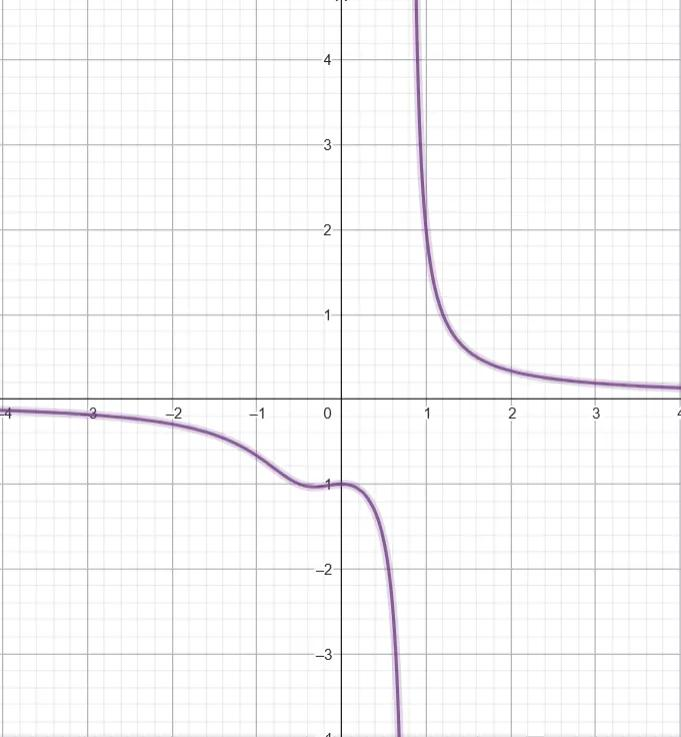
\includegraphics[width=0.86\textwidth]{imagenes/tema6_2_b.jpeg}
  \end{center}
  \newpage
  \item $\displaystyle\lim_{x\to\infty}\frac{x^2+1}{2x^3-1}$. Dividimos entre $x^3$:
  \[
  \frac{x^2+1}{2x^3-1}
  =\frac{\frac1x+\frac1{x^3}}{2-\frac1{x^3}}.
  \]
  Como $\frac1x\to0$, $\frac1{x^3}\to0$ y el denominador tiende a $2$:
  \[
  \lim_{x\to\infty}\frac{1/x+1/x^3}{2-1/x^3}
  =\frac02=\boxed{0}.
  \]
  Asíntota horizontal: $y=0$.
  \begin{center}
  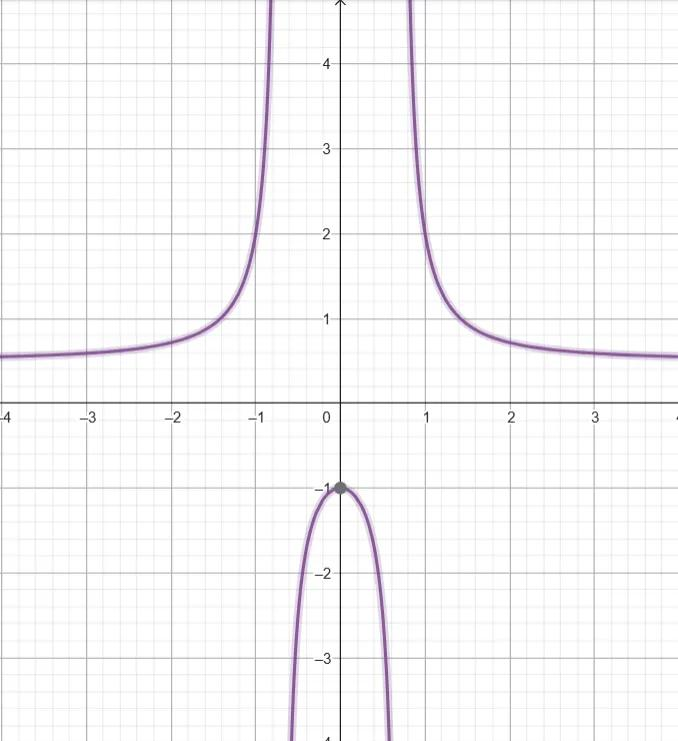
\includegraphics[width=0.86\textwidth]{imagenes/tema6_2_c.jpeg}
  \end{center}
  \newpage
  \item $\displaystyle\lim_{x\to\infty}\frac{x^2+1}{2x^2-1}$. Los grados son iguales. Dividimos entre $x^2$:
  \[
  \frac{x^2+1}{2x^2-1}
  =\frac{1+\frac1{x^2}}{2-\frac1{x^2}}.
  \]
  Cuando $x\to\infty$, $\frac1{x^2}\to0$:
  \[
  \lim_{x\to\infty}\frac{1+1/x^2}{2-1/x^2}
  =\frac{1+0}{2-0}=\boxed{\frac12}.
  \]
  Asíntota horizontal: $y=\frac12$.
  \begin{center}
  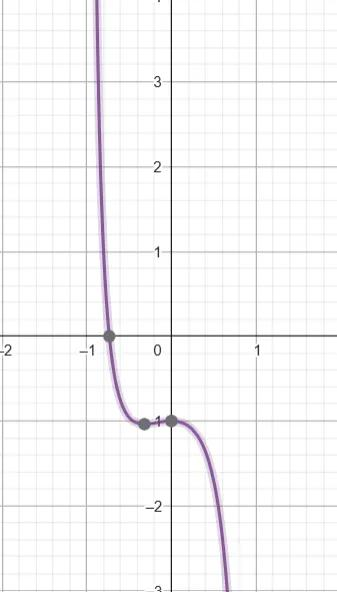
\includegraphics[width=0.65\textwidth]{imagenes/tema6_2_d.jpeg}
  \end{center}
  \newpage
  \item $\displaystyle\lim_{x\to\infty}\frac{x^5+2x^3+1}{x^2-1}$. Dividimos numerador y denominador entre $x^2$:
  \[
  \frac{x^5+2x^3+1}{x^2-1}
  =\frac{x^3+2x+\frac1{x^2}}{1-\frac1{x^2}}.
  \]
  Tenemos $2x\to+\infty$, $\frac1{x^2}\to0$ y $1-\frac1{x^2}\to1$:
  \[
  \lim_{x\to\infty}\frac{x^5+2x^3+1}{x^2-1}=+\infty.
  \]
  No existe asíntota horizontal.
  \begin{center}
  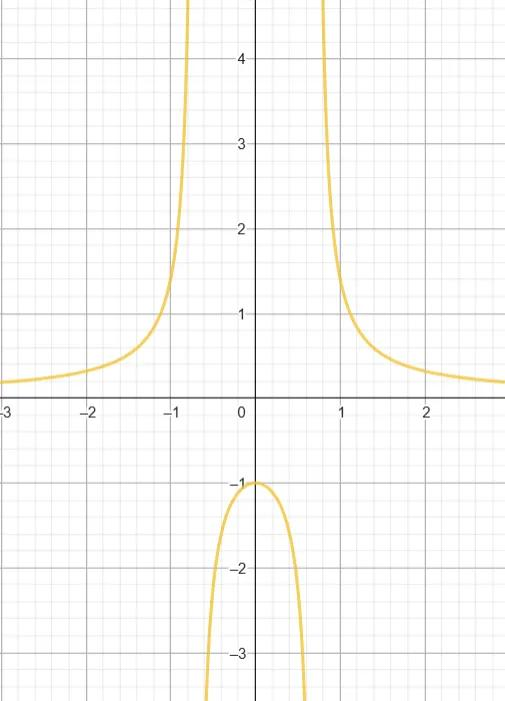
\includegraphics[width=0.86\textwidth]{imagenes/tema6_2_e.jpeg}
  \end{center}
  \newpage
  \item $\displaystyle\lim_{x\to-\infty}\frac{x^5+2x^3+1}{x^2-1}$. Dividimos entre $x^2$:
  \[
  \frac{x^5+2x^3+1}{x^2-1}
  =\frac{x^3+2x+\frac1{x^2}}{1-\frac1{x^2}}.
  \]
  Para $x\to-\infty$, $x^3\to-\infty$, $2x\to-\infty$ y $\frac1{x^2}\to0$. El denominador tiende a $1$, por lo que:
  \[
  \lim_{x\to-\infty}\frac{x^5+2x^3+1}{x^2-1}=-\infty.
  \]
  No existe asíntota horizontal.
  \begin{center}
  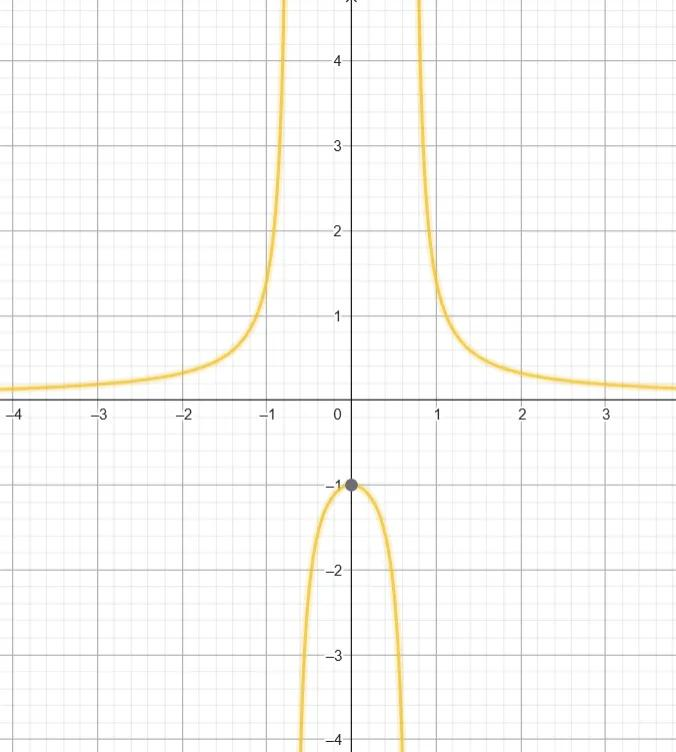
\includegraphics[width=0.86\textwidth]{imagenes/tema6_2_f.jpeg}
  \end{center}
  \newpage
  \item $\displaystyle\lim_{x\to\infty}\frac{\sqrt{x^2+1}}{2x^2-1}$. Para $x>0$, $x^2$ es positivo y podemos escribir:
  \[
  \sqrt{x^2+1}=x\sqrt{1+\frac1{x^2}}.
  \]
  Por tanto,
  \[
  \frac{\sqrt{x^2+1}}{2x^2-1}
  =\frac{\sqrt{1+1/x^2}}{2x-1/x}.
  \]
  El numerador tiende a $1$, mientras que $2x-\frac1x\to+\infty$:
  \[
  \lim_{x\to\infty}\frac{\sqrt{x^2+1}}{2x^2-1}=0.
  \]
  Asíntota horizontal: $y=0$.
  \begin{center}
  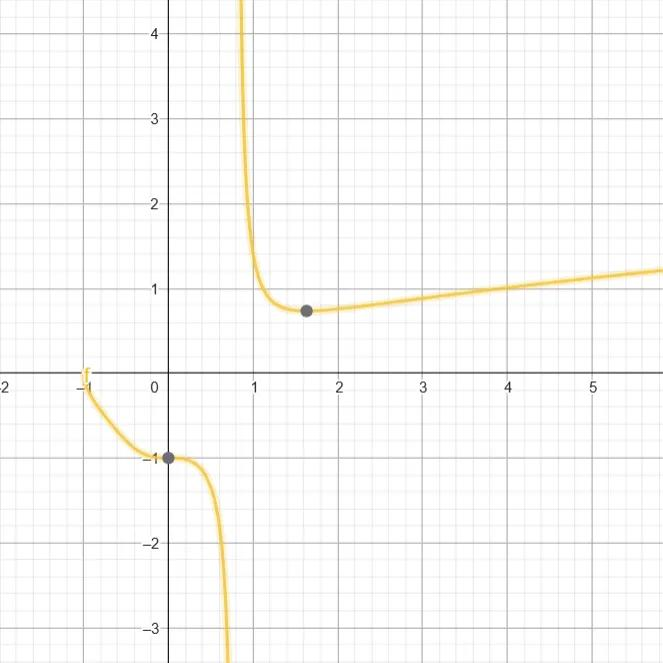
\includegraphics[width=0.86\textwidth]{imagenes/tema6_2_g.jpeg}
  \end{center}
  \newpage
  \item $\displaystyle\lim_{x\to\infty}\frac{\sqrt{x^7+1}}{2x^3-1}$. Para $x>0$:
  \[
  \sqrt{x^7+1}=x^{7/2}\sqrt{1+\frac1{x^7}},
  \qquad
  2x^3-1=x^3\left(2-\frac1{x^3}\right).
  \]
  Entonces
  \[
  \frac{\sqrt{x^7+1}}{2x^3-1}
  =\frac12\sqrt{x}\,
  \frac{\sqrt{1+1/x^7}}{1-1/(2x^3)}.
  \]
  Como $\sqrt{x}\to+\infty$ y el factor restante tiende a $1$:
  \[
  \lim_{x\to\infty}\frac{\sqrt{x^7+1}}{2x^3-1}=+\infty.
  \]
  No existe asíntota horizontal.
  \begin{center}
  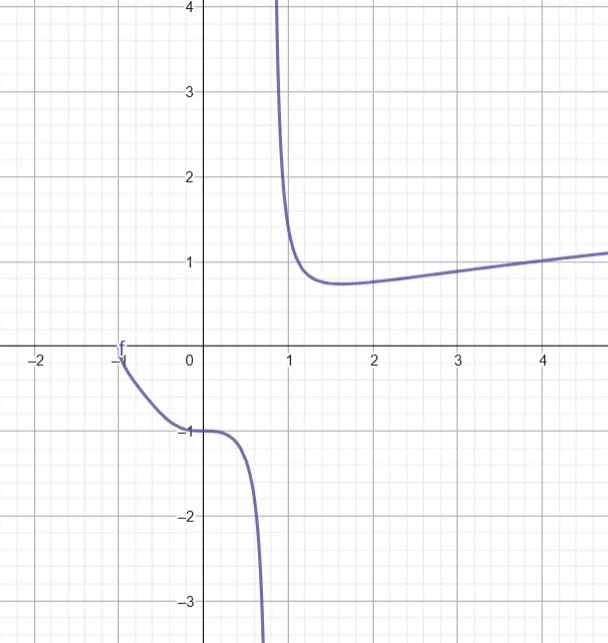
\includegraphics[width=0.86\textwidth]{imagenes/tema6_2_h.jpeg}
  \end{center}
  \newpage
  \item $\displaystyle\lim_{x\to-\infty}\frac{\sqrt{x^7+1}}{2x^3-1}$. La raíz exige $x^7+1\geq0$. Como $x^7\leq-1$ cuando $x\leq-1$, tenemos:
  \[
  x^7+1\geq0\quad\Longleftrightarrow\quad x^7\geq-1
  \quad\Longleftrightarrow\quad x\geq-1.
  \]
  Por tanto, no existen valores reales de la función a la izquierda de $-1$ arbitrariamente cercanos a $-\infty$. El límite no está definido en los reales.
  \begin{center}
  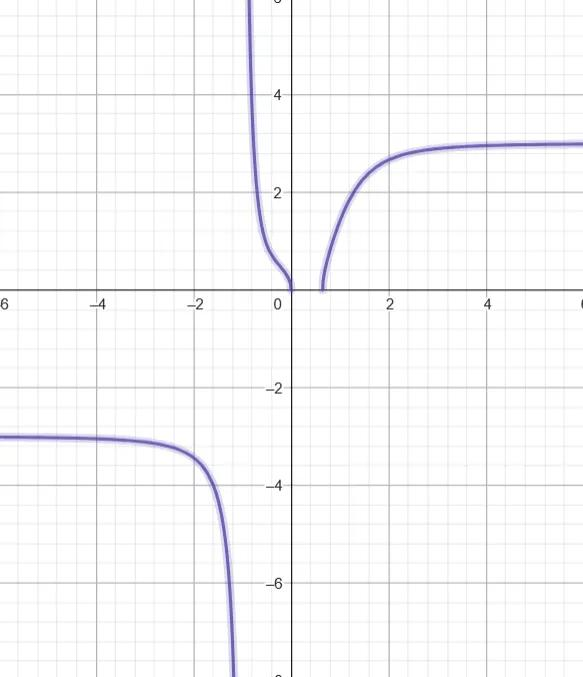
\includegraphics[width=0.86\textwidth]{imagenes/tema6_2_i.jpeg}
  \end{center}
  \newpage
  \item $\displaystyle\lim_{x\to\infty}\frac{\sqrt{9x^6-x}}{x^3+1}$. Para $x>0$, $\sqrt{x^6}=x^3$. Extraemos $x^6$ dentro de la raíz:
  \[
  \sqrt{9x^6-x}=x^3\sqrt{9-\frac1{x^5}}.
  \]
  Dividimos también el denominador entre $x^3$:
  \[
  \frac{\sqrt{9x^6-x}}{x^3+1}
  =\frac{\sqrt{9-1/x^5}}{1+1/x^3}.
  \]
  Como $\frac1{x^5}\to0$ y $\frac1{x^3}\to0$:
  \[
  \lim_{x\to\infty}\frac{\sqrt{9x^6-x}}{x^3+1}
  =\frac{\sqrt{9}}1=\boxed3.
  \]
  Asíntota horizontal: $y=3$.
  \begin{center}
  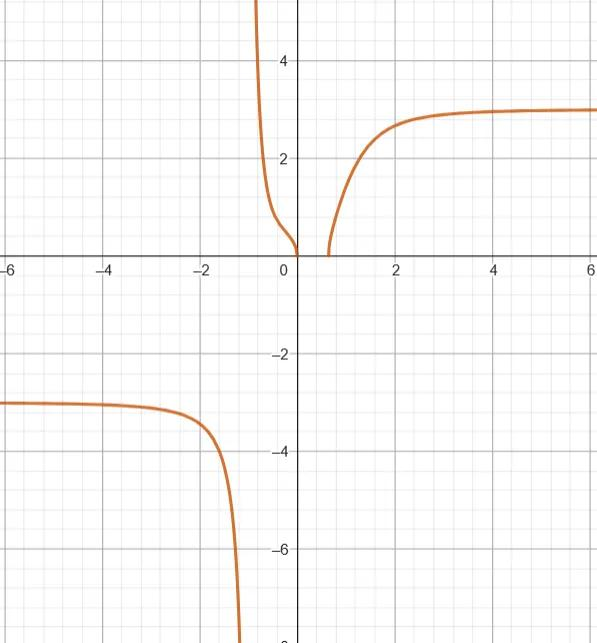
\includegraphics[width=0.86\textwidth]{imagenes/tema6_2_j.jpeg}
  \end{center}
  \newpage
  \item $\displaystyle\lim_{x\to-\infty}\frac{\sqrt{9x^6-x}}{x^3+1}$. Cuando $x<0$, $x^6=|x^3|^2$ y al extraer el factor se tiene:
  \[
  \sqrt{9x^6-x}=|x^3|\sqrt{9-\frac1{x^5}}
  =-x^3\sqrt{9-\frac1{x^5}}.
  \]
  Dividiendo numerador y denominador entre $x^3$:
  \[
  \frac{\sqrt{9x^6-x}}{x^3+1}
  =\frac{-\sqrt{9-1/x^5}}{1+1/x^3}.
  \]
  Como $1/x^5\to0$ y $1/x^3\to0$:
  \[
  \lim_{x\to-\infty}\frac{\sqrt{9x^6-x}}{x^3+1}
  =-\sqrt9=\boxed{-3}.
  \]
  Asíntota horizontal: $y=-3$.
  \begin{center}
  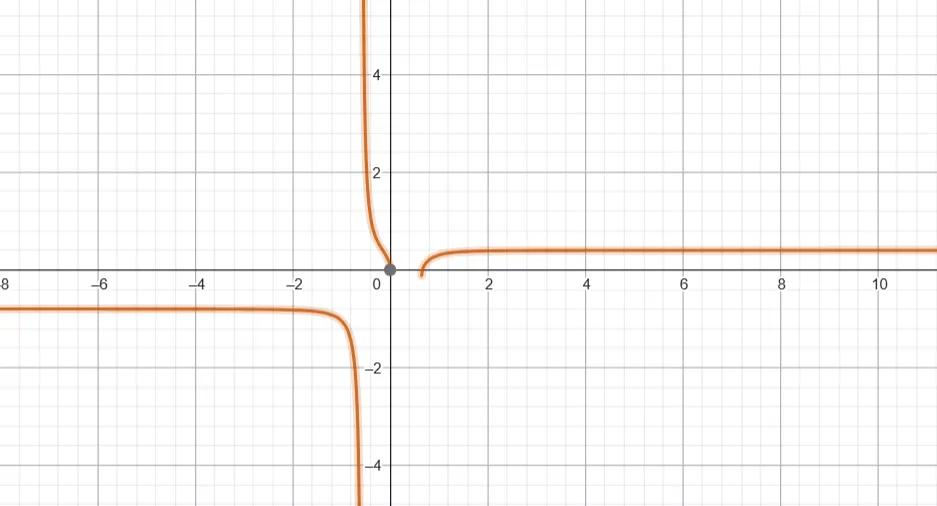
\includegraphics[width=0.86\textwidth]{imagenes/tema6_2_k.jpeg}
  \end{center}
  \newpage
  \item $\displaystyle\lim_{x\to\infty}\frac{\sqrt{9x^6-x}-x^3}{5x^3+1}$. Para $x>0$, factorizamos $x^3$ en ambos términos:
  \[
  \frac{\sqrt{9x^6-x}-x^3}{5x^3+1}
  =\frac{x^3\sqrt{9-1/x^5}-x^3}{x^3(5+1/x^3)}
  =\frac{\sqrt{9-1/x^5}-1}{5+1/x^3}.
  \]
  Como $1/x^5\to0$ y $1/x^3\to0$:
  \[
  \lim_{x\to\infty}\frac{\sqrt{9-1/x^5}-1}{5+1/x^3}
  =\frac{3-1}{5}=\boxed{\frac25}.
  \]
  Asíntota horizontal: $y=\frac25$.
  \begin{center}
  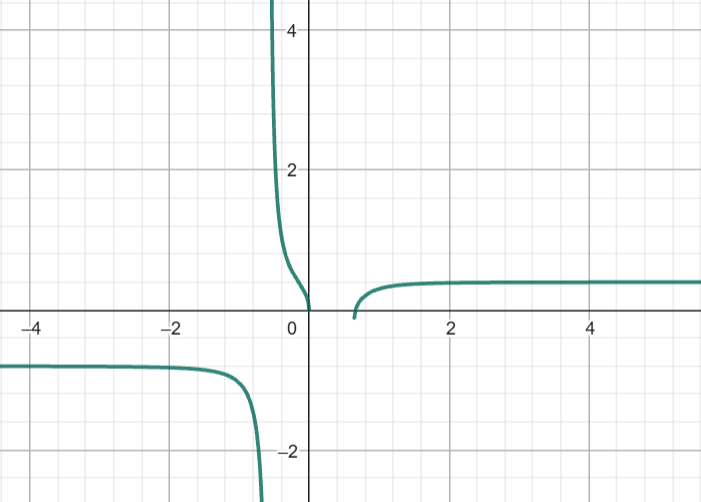
\includegraphics[width=0.86\textwidth]{imagenes/tema6_2_l.png}
  \end{center}
  \newpage
  \item $\displaystyle\lim_{x\to-\infty}\frac{\sqrt{9x^6-x}-x^3}{5x^3+1}$. Para $x<0$, $\sqrt{9x^6-x}= -x^3\sqrt{9-1/x^5}$:
  \[
  \frac{\sqrt{9x^6-x}-x^3}{5x^3+1}
  =\frac{-x^3\sqrt{9-1/x^5}-x^3}{x^3(5+1/x^3)}
  =\frac{-\sqrt{9-1/x^5}-1}{5+1/x^3}.
  \]
  Al aplicar los límites de $1/x^5$ y $1/x^3$:
  \[
  \lim_{x\to-\infty}\frac{-\sqrt{9-1/x^5}-1}{5+1/x^3}
  =\frac{-3-1}{5}=\boxed{-\frac45}.
  \]
  Asíntota horizontal: $y=-\frac45$.
  \begin{center}
  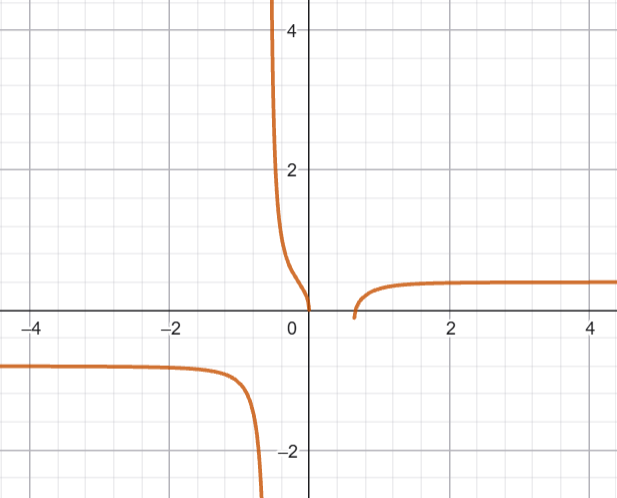
\includegraphics[width=0.86\textwidth]{imagenes/tema6_2_m.png}
  \end{center}
  \newpage
\end{enumerate}

% =================================================
% TEMA 7
% =================================================

\newpage
\section{Tema 7. Definición de derivada}

Encuentre la derivada de las siguientes funciones utilizando la definición de derivada como límite:
\[
f'(x)=\lim_{h\to0}\frac{f(x+h)-f(x)}{h}.
\]
\textbf{Método:} primero se calcula $f(x+h)$ sustituyendo $x+h$ en la variable original, luego se resta $f(x)$, se simplifica y se factoriza $h$ para cancelar $h$ del denominador. El último paso es evaluar el límite cuando $h\to0$.
\begin{enumerate}[label=\alph*)]
  \item $f(x)=x$:
  \[
  f'(x)=\lim_{h\to0}\frac{(x+h)-x}{h}
  =\lim_{h\to0}\frac{x+h-x}{h}
  =\lim_{h\to0}\frac{h}{h}
  =\boxed{1}.
  \]
  \item $f(x)=x^2$:
  \[
  \begin{aligned}
  f'(x)&=\lim_{h\to0}\frac{(x+h)^2-x^2}{h}\\
  &=\lim_{h\to0}\frac{x^2+2xh+h^2-x^2}{h}\\
  &=\lim_{h\to0}\frac{h(2x+h)}h
  =\lim_{h\to0}(2x+h)=\boxed{2x}.
  \end{aligned}
  \]
  \item $f(x)=x^3$:
  \[
  \begin{aligned}
  f'(x)&=\lim_{h\to0}\frac{(x+h)^3-x^3}{h}\\
  &=\lim_{h\to0}\frac{x^3+3x^2h+3xh^2+h^3-x^3}{h}\\
  &=\lim_{h\to0}(3x^2+3xh+h^2)=\boxed{3x^2}.
  \end{aligned}
  \]
  \item $f(x)=x^4$:
  \[
  \begin{aligned}
  f'(x)&=\lim_{h\to0}\frac{(x+h)^4-x^4}{h}\\
  &=\lim_{h\to0}\frac{4x^3h+6x^2h^2+4xh^3+h^4}{h}\\
  &=\lim_{h\to0}(4x^3+6x^2h+4xh^2+h^3)=\boxed{4x^3}.
  \end{aligned}
  \]
  \item $f(x)=x^5$:
  \[
  \begin{aligned}
  f'(x)&=\lim_{h\to0}\frac{(x+h)^5-x^5}{h}\\
  &=\lim_{h\to0}(5x^4+10x^3h+10x^2h^2+5xh^3+h^4)
  =\boxed{5x^4}.
  \end{aligned}
  \]
  \item $f(x)=3$:
  $\displaystyle f'(x)=\lim_{h\to0}\frac{3-3}{h}=\boxed{0}$.
  \item $f(x)=3x^2$:
  \[
  \begin{aligned}
  f'(x)&=\lim_{h\to0}\frac{3(x+h)^2-3x^2}{h}\\
  &=\lim_{h\to0}\frac{3(2xh+h^2)}h
  =\lim_{h\to0}(6x+3h)=\boxed{6x}.
  \end{aligned}
  \]
  \item $f(x)=2x^2+4x+1$:
  \[
  \begin{aligned}
  f'(x)&=\lim_{h\to0}\frac{2(x+h)^2+4(x+h)+1-(2x^2+4x+1)}h\\
  &=\lim_{h\to0}\frac{4xh+2h^2+4h}{h}
  =\lim_{h\to0}(4x+2h+4)=\boxed{4x+4}.
  \end{aligned}
  \]
  \item $f(x)=\dfrac1x$:
  \[
  \begin{aligned}
  f'(x)&=\lim_{h\to0}\frac{\frac1{x+h}-\frac1x}{h}\\
  &=\lim_{h\to0}\frac{\frac{x-(x+h)}{x(x+h)}}h
  =\lim_{h\to0}\frac{-h}{h\,x(x+h)}
  =\lim_{h\to0}\frac{-1}{x(x+h)}
  =\boxed{-\frac1{x^2}},
  \end{aligned}
  \]
  siempre que $x\neq0$.
  \item $f(x)=\dfrac1{x^2}$:
  \[
  \begin{aligned}
  f'(x)&=\lim_{h\to0}\frac{\frac1{(x+h)^2}-\frac1{x^2}}h\\
  &=\lim_{h\to0}\frac{x^2-(x+h)^2}{h\,x^2(x+h)^2}\\
  &=\lim_{h\to0}\frac{-2xh-h^2}{h\,x^2(x+h)^2}\\
  &=\lim_{h\to0}\frac{-(2x+h)}{x^2(x+h)^2}
  =\boxed{-\frac2{x^3}},\qquad x\neq0.
  \end{aligned}
  \]
  \item $f(x)=\dfrac1{x^3}$:
  \[
  \begin{aligned}
  f'(x)&=\lim_{h\to0}
  \frac{\frac1{(x+h)^3}-\frac1{x^3}}h\\
  &=\lim_{h\to0}\frac{x^3-(x+h)^3}{h\,x^3(x+h)^3}\\
  &=\lim_{h\to0}\frac{-3x^2-3xh-h^2}{x^3(x+h)^3}
  =\boxed{-\frac3{x^4}}.
  \end{aligned}
  \]
  \item $f(x)=\sqrt{x}$:
  \[
  \begin{aligned}
  f'(x)&=\lim_{h\to0}\frac{\sqrt{x+h}-\sqrt{x}}h\\
  &=\lim_{h\to0}
  \frac{(\sqrt{x+h}-\sqrt{x})(\sqrt{x+h}+\sqrt{x})}
  {h(\sqrt{x+h}+\sqrt{x})}\\
  &=\lim_{h\to0}\frac{(x+h)-x}{h(\sqrt{x+h}+\sqrt{x})}\\
  &=\lim_{h\to0}\frac1{\sqrt{x+h}+\sqrt{x}}
  =\boxed{\frac1{2\sqrt{x}}},\qquad x>0.
  \end{aligned}
  \]
  \item $f(x)=\dfrac1{\sqrt{x}}$:
  \[
  f'(x)=\lim_{h\to0}\frac{\frac1{\sqrt{x+h}}-\frac1{\sqrt{x}}}{h}
  =\lim_{h\to0}\frac{-1}{\sqrt{x}\sqrt{x+h}(\sqrt{x}+\sqrt{x+h})}
  =\boxed{-\frac{1}{2x^{3/2}}},\quad x>0.
  \]
\end{enumerate}

% =================================================
% TEMA 8
% =================================================

\newpage
\section{Tema 8. Reglas de derivación}

Encuentre las derivadas de las siguientes funciones con ayuda de tu formulario de reglas de derivación. En los incisos con $\log x$ se interpreta el logaritmo común (base 10).
\textbf{Criterios utilizados:}
\begin{itemize}
  \item Regla del producto: $(uv)'=u'v+uv'$.
  \item Regla del cociente: $\left(\frac uv\right)'=\frac{u'v-uv'}{v^2}$.
  \item Regla de la cadena: $(f(g(x)))'=f'(g(x))g'(x)$.
  \item Después de derivar se simplifica cada factor y se identifica el factor común para presentar el resultado de forma factorizada.
\end{itemize}
\begin{enumerate}[label=\alph*)]
  \item $f(x)=3\sin x+4\cos x$.\\
  \[
  f'(x)=3(\sin x)'+4(\cos x)'
  =3\cos x+4(-\sin x)
  =\boxed{3\cos x-4\sin x}.
  \]
  \item $f(x)=3x^5+\dfrac15x^4+\dfrac23x^3-\dfrac57x^2+\dfrac87x-\dfrac13$.\\
  $\boxed{f'(x)=15x^4+\dfrac45x^3+2x^2-\dfrac{10}{7}x+\dfrac87}$.
  \item $f(x)=\dfrac3x+\dfrac1{x^2}-\dfrac1{5x^2}-\dfrac2{3x^3}$.\\
  Derivando término a término: $\boxed{f'(x)=-\dfrac3{x^2}-\dfrac8{5x^3}+\dfrac2{x^4}}$.
  \item $f(x)=3\sqrt{x}+\sqrt[4]{x}$.\\
  \[
  f(x)=3x^{1/2}+x^{1/4}
  \quad\Longrightarrow\quad
  f'(x)=3\left(\frac12x^{-1/2}\right)
  +\frac14x^{-3/4}
  =\boxed{\frac{3}{2\sqrt{x}}+\frac{1}{4x^{3/4}}}.
  \]
  \item $f(x)=\sqrt[5]{x^2}-\dfrac{3}{\sqrt[5]{x^2}}=x^{2/5}-3x^{-2/5}$.\\
  \[
  f'(x)=\frac25x^{2/5-1}-3\left(-\frac25x^{-2/5-1}\right)
  =\frac25x^{-3/5}+\frac65x^{-7/5}.
  \]
  \item $f(x)=\dfrac23\log_2x+3\ln|x|$.\\
  \[
  (\log_2x)'=\frac1{x\ln2},\qquad(\ln|x|)'=\frac1x,
  \]
  \[
  f'(x)=\frac23\left(\frac1{x\ln2}\right)+3\left(\frac1x\right)
  =\boxed{\frac{2}{3x\ln2}+\frac3x}.
  \]
  \item $f(x)=x^2\log x$. Por regla del producto, con $u=x^2$ y $v=\log x$:
  \[
  u'=2x,\qquad v'=\frac1{x\ln10}.
  \]
  \[
  f'=u'v+uv'
  =2x\log x+x^2\left(\frac1{x\ln10}\right)
  =\boxed{2x\log x+\frac{x}{\ln10}}.
  \]
  \item $f(x)=e^x\cos x$.\\
  \[
  f'(x)=(e^x)'\cos x+e^x(\cos x)'
  =e^x\cos x-e^x\sin x
  =\boxed{e^x(\cos x-\sin x)}.
  \]
  \item $f(x)=x^2e^x\cos x$. Aplicamos primero la regla del producto a $u=x^2$ y $v=e^x\cos x$:
  \[
  u'=2x,\qquad v'=e^x\cos x-e^x\sin x=e^x(\cos x-\sin x).
  \]
  \[
  f'=2x(e^x\cos x)+x^2e^x(\cos x-\sin x)
  =\boxed{e^x\left[(2x+x^2)\cos x-x^2\sin x\right]}.
  \]
  \item $f(x)=\dfrac{x^2}{\ln|x|}$. Por regla del cociente, $u=x^2$ y $v=\ln|x|$:
  \[
  u'=2x,\qquad v'= \frac1x.
  \]
  \[
  f'=\frac{u'v-uv'}{v^2}
  =\frac{2x\ln|x|-x^2(1/x)}{(\ln|x|)^2}
  =\boxed{\frac{2x\ln|x|-x}{(\ln|x|)^2}},
  \]
  para $x\neq0,\pm1$.
  \item $f(x)=\dfrac{x^2\cos x}{e^x}$. Escribiendo $f=x^2e^{-x}\cos x$, derivamos primero $x^2e^{-x}$:
  \[
  (x^2e^{-x})'=2xe^{-x}-x^2e^{-x}=e^{-x}(2x-x^2).
  \]
  Aplicamos nuevamente el producto con $\cos x$:
  \[
  f'=e^{-x}(2x-x^2)\cos x+x^2e^{-x}(-\sin x)
  =\boxed{e^{-x}\left[(2x-x^2)\cos x-x^2\sin x\right]}.
  \]
  \item $f(x)=\dfrac{x^2\cos x}{e^x\sinh x}$.\\
  $\boxed{f'(x)=\dfrac{2x\cos x-x^2\sin x-x^2\cos x-x^2\cos x\coth x}{e^x\sinh x}}$.
  \item $f(x)=\ln x^3$. Como $\ln(x^3)=3\ln x$ para $x>0$:
  \[
  f'(x)=\frac{d}{dx}(3\ln x)=3\left(\frac1x\right)
  =\boxed{\frac3x}.
  \]
  \item $f(x)=\sqrt[3]{\ln x}=(\ln x)^{1/3}$. Por la regla de la potencia combinada con la cadena:
  \[
  f'=\frac13(\ln x)^{-2/3}\frac{d}{dx}(\ln x)
  =\frac13(\ln x)^{-2/3}\frac1x
  =\boxed{\dfrac{1}{3x(\ln x)^{2/3}}},
  \]
  para $x>0$ y $\ln x\neq0$.
  \item $f(x)=\sin 2x+\cos 3x$.\\
  \[
  f'(x)=\cos(2x)(2)+[-\sin(3x)](3)
  =\boxed{2\cos2x-3\sin3x}.
  \]
  \item $f(x)=\sin(x^2)+e^{2x+3}$.\\
  \[
  f'(x)=\cos(x^2)(2x)+e^{2x+3}(2)
  =\boxed{2x\cos(x^2)+2e^{2x+3}}.
  \]
  \item $f(x)=e^{\sin(x^2)}$. Aplicamos la cadena tres veces:
  \[
  e^u\text{ con }u=\sin(x^2),\qquad
  u'=\cos(x^2)(2x).
  \]
  \[
  f'=e^{\sin(x^2)}u'
  =\boxed{2x\cos(x^2)e^{\sin(x^2)}}.
  \]
  \item $f(x)=\cos\left(\dfrac{1-e^{2x}}{1+e^x}\right)$. Primero simplificamos el argumento:
  \[
  \frac{1-e^{2x}}{1+e^x}
  =\frac{(1-e^x)(1+e^x)}{1+e^x}
  =1-e^x.
  \]
  Entonces $f(x)=\cos(1-e^x)$ y
  \[
  f'= -\sin(1-e^x)\frac{d}{dx}(1-e^x)
  =-\sin(1-e^x)(-e^x)
  =\boxed{e^x\sin(1-e^x)}.
  \]
  \item $\displaystyle f(x)=\frac{1}{\sqrt{x+\sqrt{x+\sqrt{x+\sqrt{x+\sqrt{x}}}}}}$. Para escribir la derivada sin ocultar la regla de la cadena, definimos
  \[
  u_1=\sqrt{x},\quad u_2=\sqrt{x+u_1},\quad u_3=\sqrt{x+u_2},\quad
  u_4=\sqrt{x+u_3},\quad u_5=\sqrt{x+u_4}.
  \]
  Entonces $f=1/u_5$ y
  \[
  u_1'=\frac1{2u_1},\quad u_2'=\frac{1+u_1'}{2u_2},\quad
  u_3'=\frac{1+u_2'}{2u_3},\quad u_4'=\frac{1+u_3'}{2u_4},\quad
  u_5'=\frac{1+u_4'}{2u_5}.
  \]
  Por tanto, $\boxed{f'(x)=-\dfrac{u_5'}{u_5^2}=-\dfrac{1+u_4'}{2u_5^3}}$.
  \item $f(x)=\cos\sqrt{\sin(3x^2)+\tan(6x^3)}$. Sea $A=\sin(3x^2)+\tan(6x^3)$. Entonces $A'=6x\cos(3x^2)+18x^2\sec^2(6x^3)$ y
  $\boxed{f'(x)=-\dfrac{\sin(\sqrt A)}{2\sqrt A}\left[6x\cos(3x^2)+18x^2\sec^2(6x^3)\right]}$.
\end{enumerate}

% =================================================
% TEMA 9
% =================================================

\newpage
\section{Tema 9. Máximos y mínimos}

\subsection*{1.- Para cada una de las siguientes funciones encuentre: los valores máximos, los valores mínimos, las asíntotas verticales, los intervalos en que es creciente, los intervalos en que es decreciente, los puntos de inflexión, los intervalos en que es cóncava y los intervalos en que es convexa. Muestra la gráfica de la función.}

\textbf{Criterio:} los puntos críticos se obtienen de $f'(x)=0$ o de los puntos donde $f'$ no existe dentro del dominio. La concavidad se determina con el signo de $f''(x)$.

\begin{enumerate}[label=\alph*)]
  \item $f(x)=x^3-12x+2$.
  \[
  f'(x)=3x^2-12=3(x-2)(x+2),\qquad f''(x)=6x.
  \]
  Los puntos críticos son $x=-2$ y $x=2$. El signo de $f'$ da:
  \begin{itemize}
    \item Creciente en $(-\infty,-2)\cup(2,+\infty)$.
    \item Decreciente en $(-2,2)$.
  \end{itemize}
  $f(-2)=18$ es un máximo local y $f(2)=-14$ es un mínimo local. No tiene asíntotas verticales. Como $f''(x)=0$ en $x=0$ y cambia de signo, hay punto de inflexión $(0,2)$. Es cóncava hacia abajo en $(-\infty,0)$ y convexa hacia arriba en $(0,+\infty)$. No tiene máximo ni mínimo absoluto porque es una cúbica no acotada.
  \begin{center}
  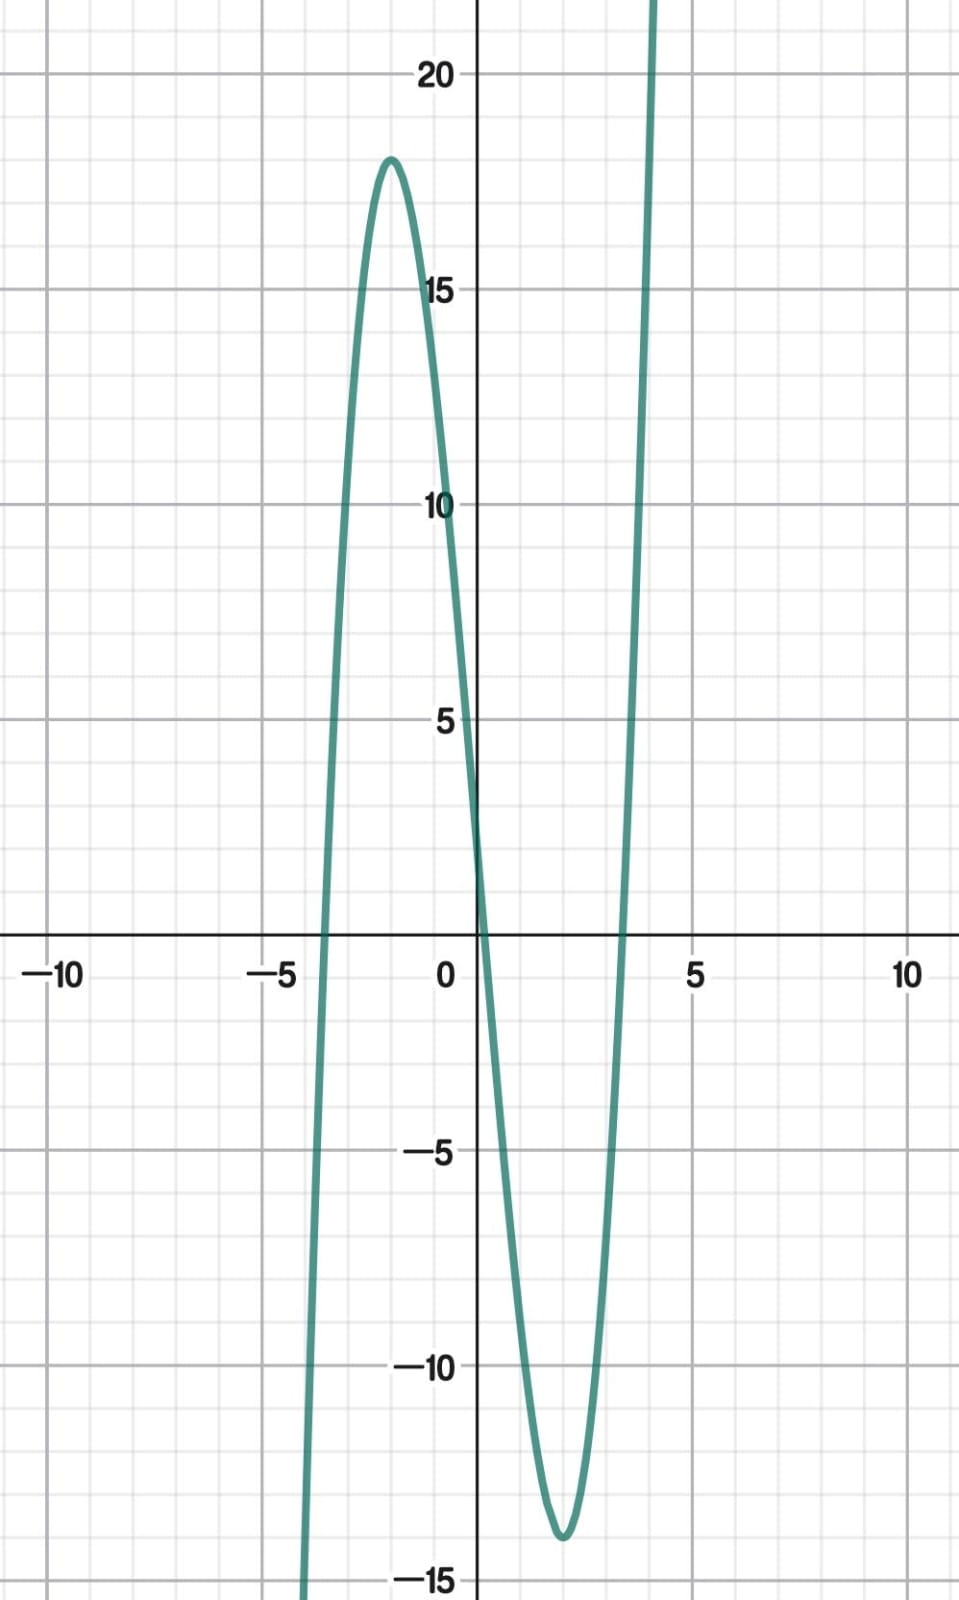
\includegraphics[width=0.86\textwidth]{imagenes/tema9_1_a.jpeg}
  \end{center}

  \item $f(x)=x^3-3x^2+1$.
  \[
  f'(x)=3x^2-6x=3x(x-2),\qquad f''(x)=6x-6.
  \]
  Los puntos críticos son $x=0$ y $x=2$:
  \begin{itemize}
    \item Creciente en $(-\infty,0)\cup(2,+\infty)$.
    \item Decreciente en $(0,2)$.
  \end{itemize}
  $f(0)=1$ es máximo local y $f(2)=-3$ es mínimo local. No tiene asíntotas verticales. $f''(x)=0$ en $x=1$ y cambia de signo; el punto de inflexión es $(1,-1)$. Es cóncava hacia abajo en $(-\infty,1)$ y convexa hacia arriba en $(1,+\infty)$. No existen extremos absolutos porque la función no está acotada.
  \begin{center}
  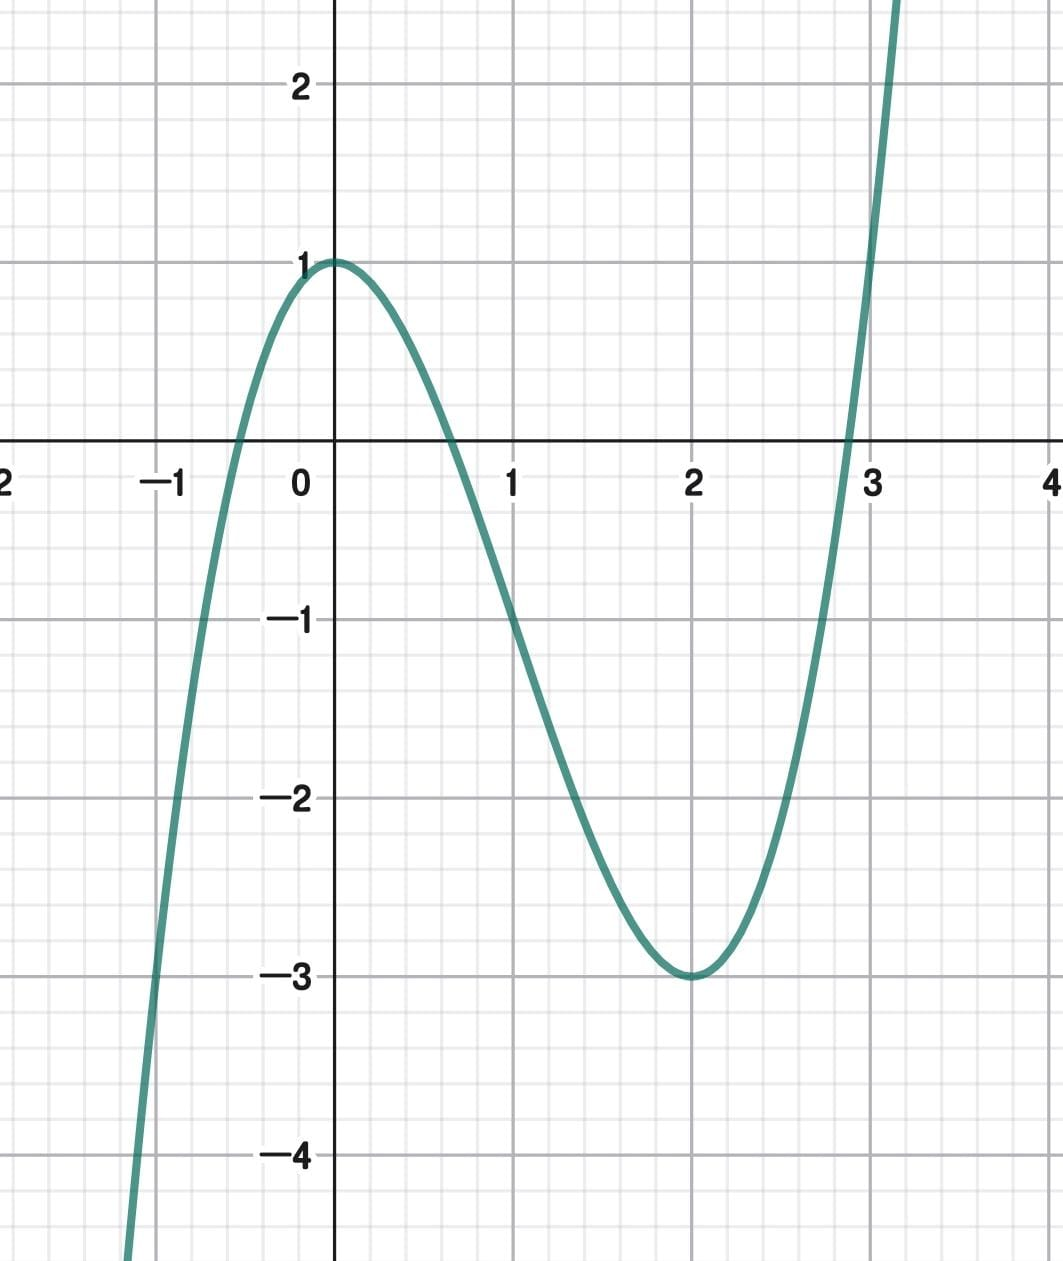
\includegraphics[width=0.86\textwidth]{imagenes/tema9_1_b.jpeg}
  \end{center}

  \item $f(x)=\dfrac{x^2}{x^2-1}$.
  \[
  f'(x)=\frac{-2x}{(x^2-1)^2},\qquad
  f''(x)=\frac{2(3x^2+1)}{(x^2-1)^3}.
  \]
  El dominio es $\R\setminus\{-1,1\}$. Por ello tiene asíntotas verticales $x=-1$ y $x=1$. Como el denominador de $f'$ es positivo en todo el dominio, el signo depende de $-x$:
  \begin{itemize}
    \item Creciente en $(-\infty,-1)\cup(-1,0)$.
    \item Decreciente en $(0,1)\cup(1,+\infty)$.
  \end{itemize}
  En $x=0$, $f(0)=0$ y la derivada cambia de positiva a negativa: hay un máximo local de valor $0$. No existe mínimo local ni máximo o mínimo absoluto (la función no está acotada cerca de las asíntotas). El numerador de $f''$ siempre es positivo, así que es convexa hacia arriba en $(-\infty,-1)\cup(1,+\infty)$ y cóncava hacia abajo en $(-1,1)$. No tiene puntos de inflexión: $f''$ no se anula y $x=\pm1$ no pertenecen al dominio.
  \begin{center}
  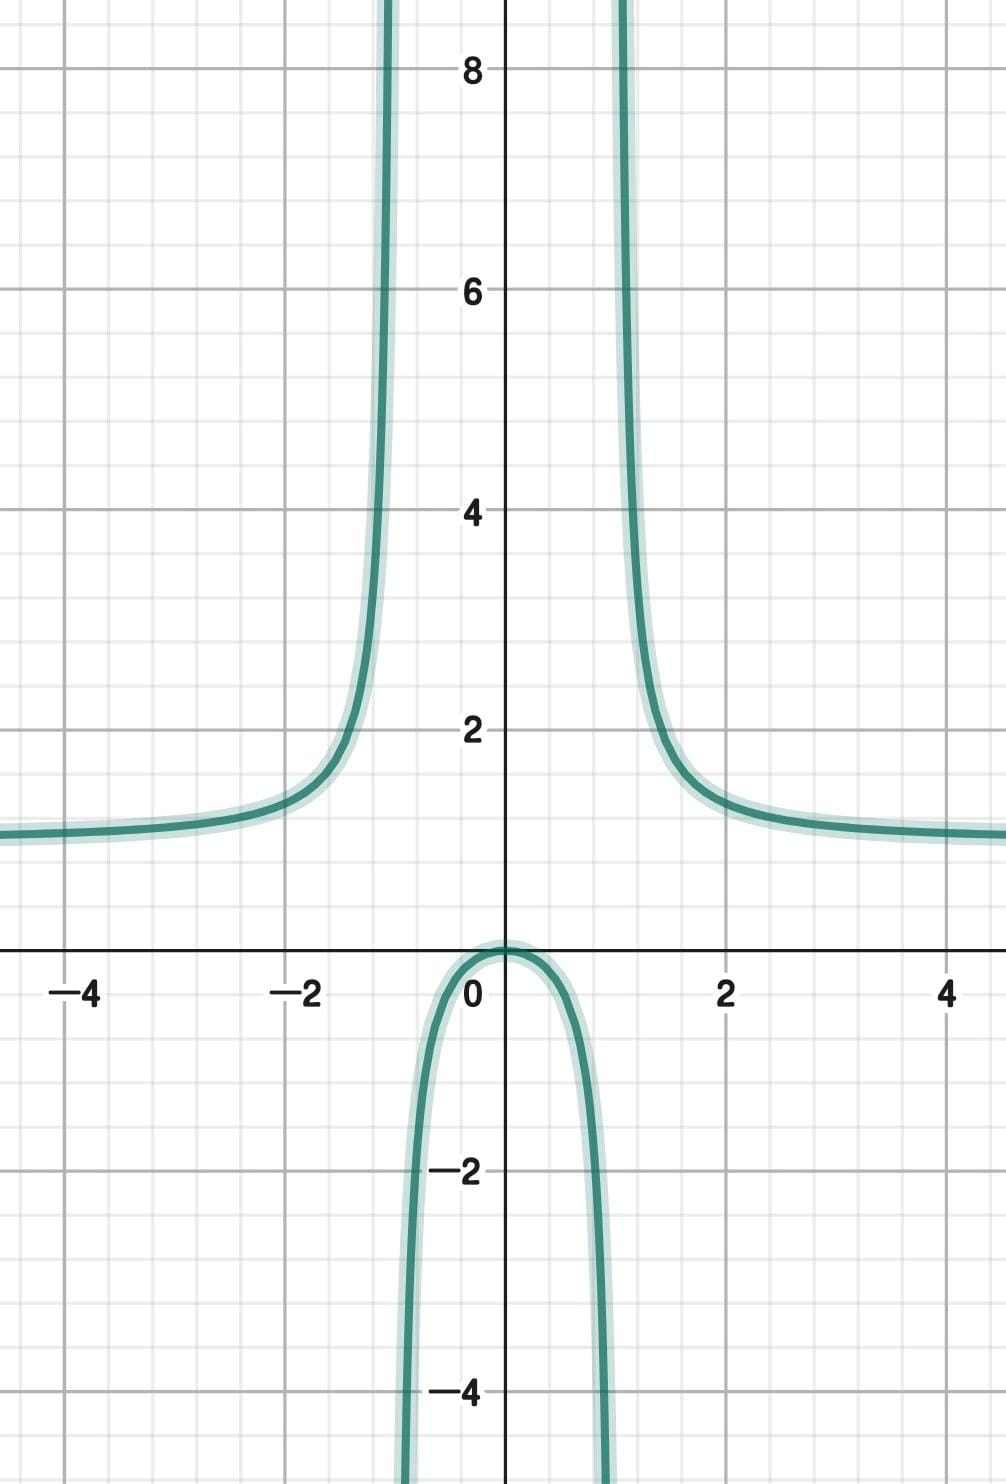
\includegraphics[width=0.86\textwidth]{imagenes/tema9_1_c.jpeg}
  \end{center}
\end{enumerate}

\subsection*{2.- Se dispone de $1200\,\mathrm{cm}^2$ de material para hacer una caja con una base cuadrada y sin tapa. Encuentre el mayor volumen posible de la caja.}
Sea $x$ el lado de la base cuadrada y $h$ la altura. El área disponible es la base más cuatro caras:
\[
x^2+4xh=1200\quad\Longrightarrow\quad h=\frac{1200-x^2}{4x}.
\]
El volumen es
\[
V(x)=x^2h=\frac{1200x-x^3}{4},\qquad 0<x<\sqrt{1200}.
\]
Derivamos e igualamos a cero:
\[
V'(x)=300-\frac34x^2=0
\quad\Longrightarrow\quad x^2=400\quad\Longrightarrow\quad x=20\text{ cm}.
\]
La altura se obtiene sustituyendo el lado:
\[
h=\frac{1200-20^2}{4(20)}
=\frac{1200-400}{80}
=\frac{800}{80}=10\text{ cm}.
\]
\[
V_{\max}=20^2(10)=400(10)=4000\text{ cm}^3.
\]
Además, $V''(x)=-\frac32x<0$ en el dominio, por lo que se trata de un máximo.
\respuesta{\text{Base: }20\text{ cm}\times20\text{ cm};\quad h=10\text{ cm};\quad V_{\max}=4000\text{ cm}^3}

\subsection*{3.- Se dispone de una lámina de cartón cuadrada de 1.2 metros de lado. Determine las dimensiones de la caja sin tapa de volumen máximo que se puede construir recortando un cuadrado igual en cada esquina y doblando las aristas resultantes de los cortes.}
Sea $x$ el lado de cada cuadrado recortado. La caja tendrá base $(1.2-2x)\times(1.2-2x)$ y altura $x$. Por tanto,
\[
V(x)=x(1.2-2x)^2,\qquad 0<x<0.6.
\]
\[
\begin{aligned}
V'(x)&=(1.2-2x)^2+x\,[2(1.2-2x)(-2)]\\
&=(1.2-2x)\bigl[(1.2-2x)-4x\bigr]\\
&=(1.2-2x)(1.2-6x)=0.
\end{aligned}
\]
Los valores críticos son $x=0.6$ y $x=0.2$. El primero produce una caja degenerada (volumen cero); el máximo interior ocurre en $x=0.2$ m. La base mide $1.2-2(0.2)=0.8$ m por lado y la altura es $0.2$ m.\respuesta{\text{Dimensiones: }0.8\text{ m}\times0.8\text{ m}\times0.2\text{ m};\quad V_{\max}=0.128\text{ m}^3}

\subsection*{4.- Se desea construir una lata con forma de cilindro cuyo volumen sea $1000\,\mathrm{cm}^3$. Encuentre las dimensiones que minimicen el área superficial total de la lata.}
\textbf{Nota:} el área superficial total de la lata debe considerar la superficie lateral, la tapa y el fondo.

El volumen y el área total de un cilindro cerrado son
\[
\pi r^2h=1000,\qquad A=2\pi r^2+2\pi rh.
\]
Despejamos $h=1000/(\pi r^2)$ y sustituimos:
\[
A(r)=2\pi r^2+\frac{2000}{r}.
\]
\[
A'(r)=4\pi r-\frac{2000}{r^2}=0
\quad\Longrightarrow\quad r^3=\frac{500}{\pi}.
\]
Multiplicando por $r^2$:
\[
4\pi r^3-2000=0
\quad\Longrightarrow\quad
r^3=\frac{500}{\pi}.
\]
Así, $r=\sqrt[3]{500/\pi}$ y, usando la condición de volumen:
\[
h=\frac{1000}{\pi r^2}
=\frac{1000}{\pi r^2}
=2r.
\]
\[
\boxed{r=\sqrt[3]{\frac{500}{\pi}}\approx5.419\text{ cm},\qquad
h=2\sqrt[3]{\frac{500}{\pi}}\approx10.838\text{ cm}.}
\]
Estas dimensiones minimizan el área total; el resultado también se obtiene al verificar que $A''(r)=4\pi+4000/r^3>0$.

% =================================================
% TEMA 10
% =================================================

\newpage
\section{Tema 10. Introducción a las integrales}

\subsection*{1.- Resuelve las siguientes integrales definidas. Para cada una, grafique la función correspondiente e ilumine el área a la que hace referencia la integral. Haga un cálculo aproximado del área descomponiéndola en figuras geométricas básica (por ejemplo, rectángulos, cuadrados, triángulos, etc.).}
\begin{enumerate}[label=\alph*)]
  \item $\displaystyle\int_0^4(x+2)\,dx$. La región es un trapecio de bases $2$ y $6$, y altura $4$; área $\frac{2+6}{2}(4)=16$.
  \[
  \begin{aligned}
  \int_0^4(x+2)\,dx&=\int_0^4x\,dx+\int_0^4 2\,dx\\
  &=\left[\frac{x^2}{2}+2x\right]_0^4\\
  &=\left(\frac{4^2}{2}+2(4)\right)-\left(\frac{0^2}{2}+2(0)\right)\\
  &=(8+8)-0=\boxed{16}.
  \end{aligned}
  \]
  \begin{center}
  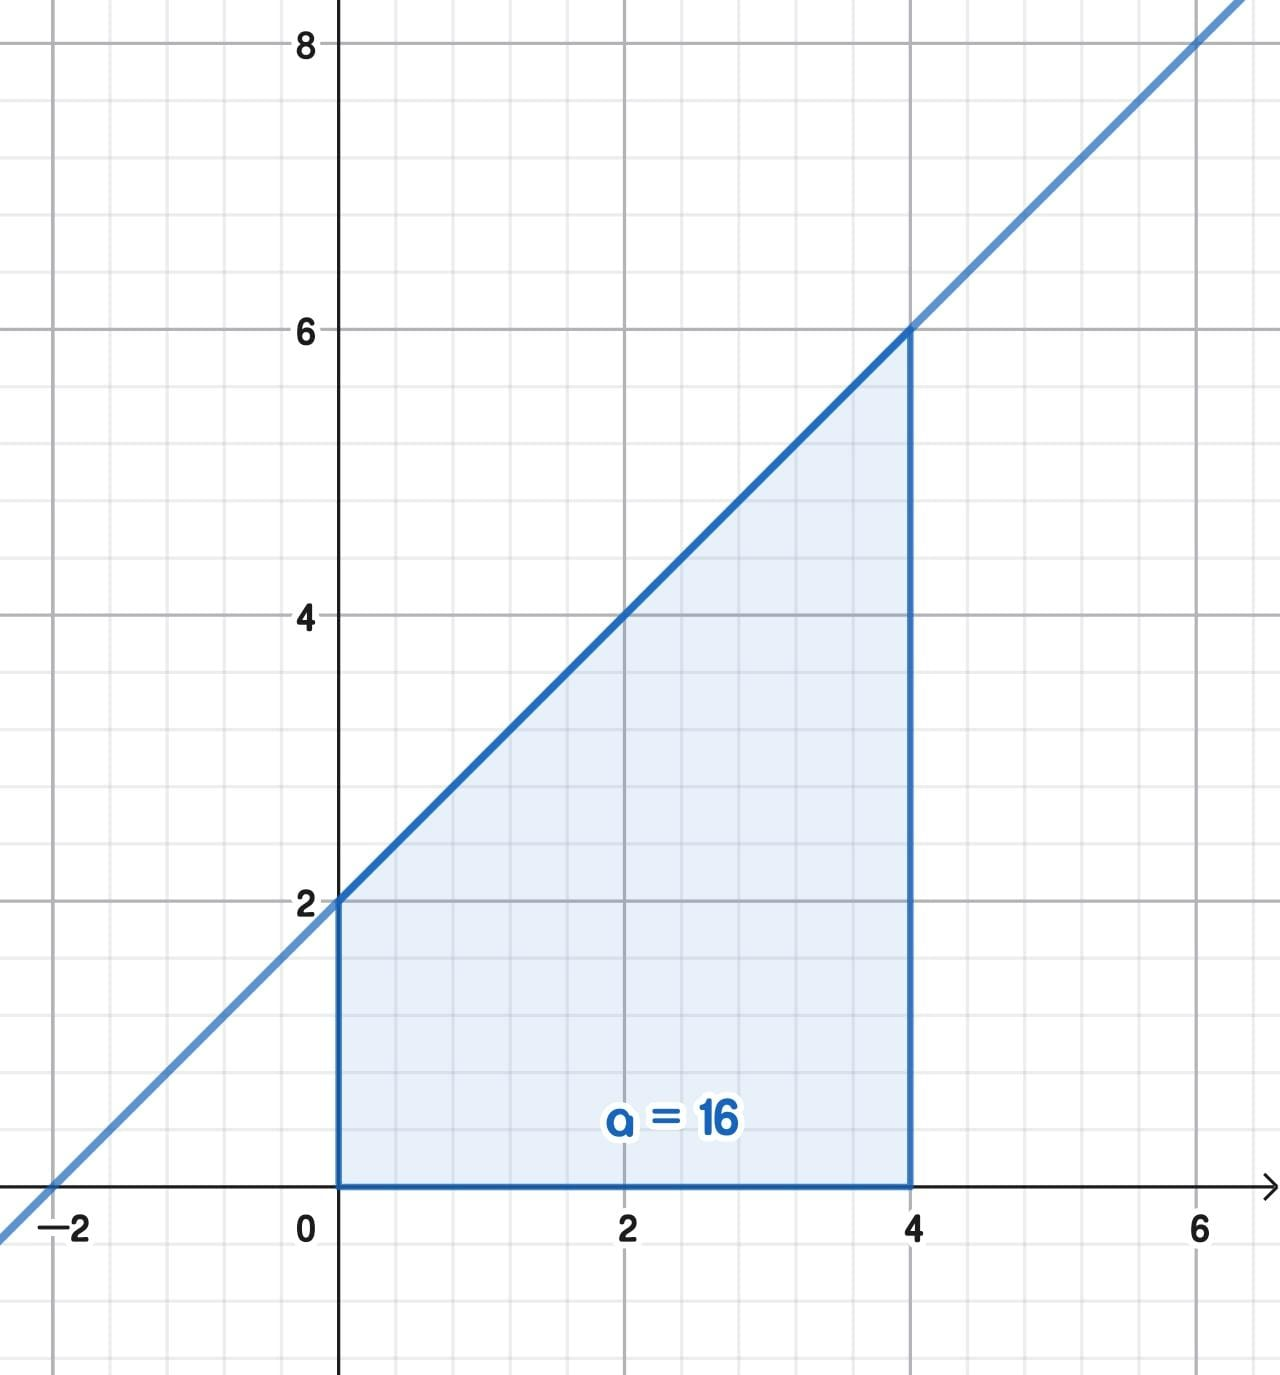
\includegraphics[width=0.86\textwidth]{imagenes/tema10_1_a.jpeg}
  \end{center}
  \item $\displaystyle\int_0^2(-x+4)\,dx$. La región es un trapecio de bases $4$ y $2$, y altura $2$; área $\frac{4+2}{2}(2)=6$.
  \[
  \begin{aligned}
  \int_0^2(-x+4)\,dx&=\left[-\frac{x^2}{2}+4x\right]_0^2\\
  &=\left(-\frac{2^2}{2}+4(2)\right)-\left(-\frac{0^2}{2}+4(0)\right)\\
  &=(-2+8)-0=\boxed{6}.
  \end{aligned}
  \]
  \begin{center}
  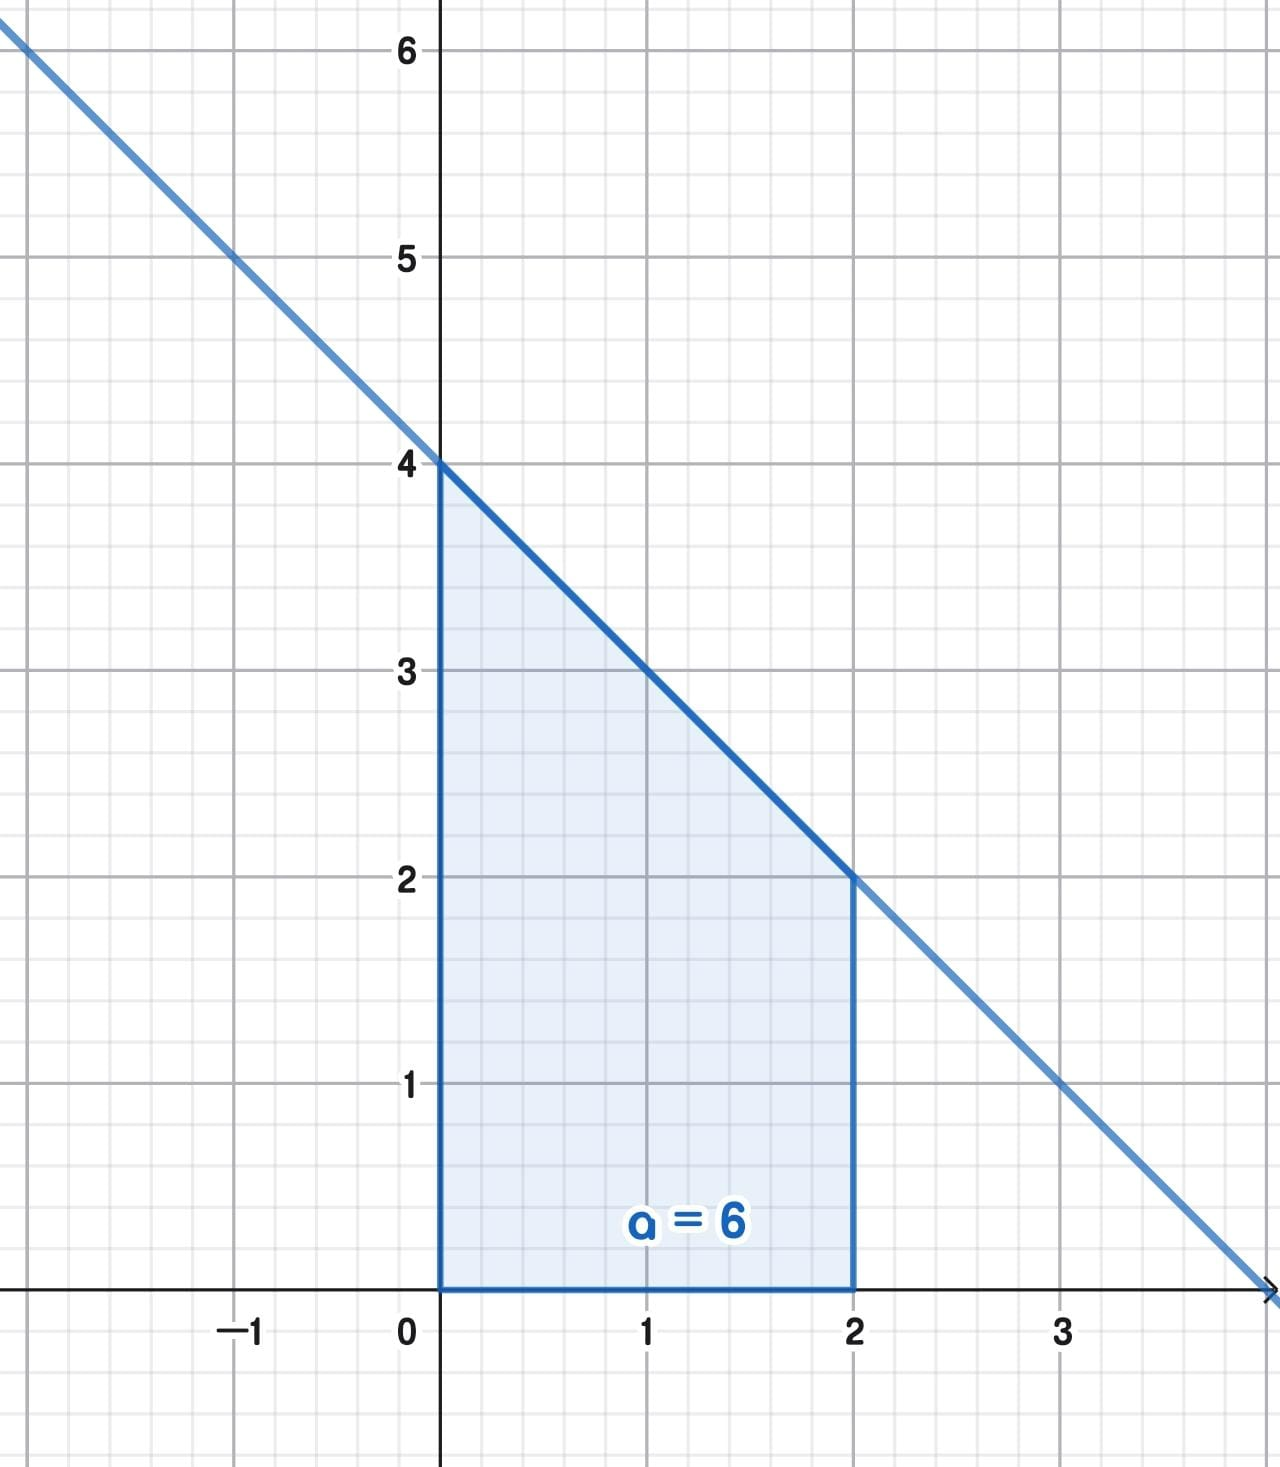
\includegraphics[width=0.86\textwidth]{imagenes/tema10_1_b.jpeg}
  \end{center}
  \newpage
  \item $\displaystyle\int_0^6 5\,dx$. La región es un rectángulo de base $6$ y altura $5$; área $6(5)=30$.
  \[
  \begin{aligned}
  \int_0^6 5\,dx&=[5x]_0^6\\
  &=5(6)-5(0)=30-0=\boxed{30}.
  \end{aligned}
  \]
  \begin{center}
  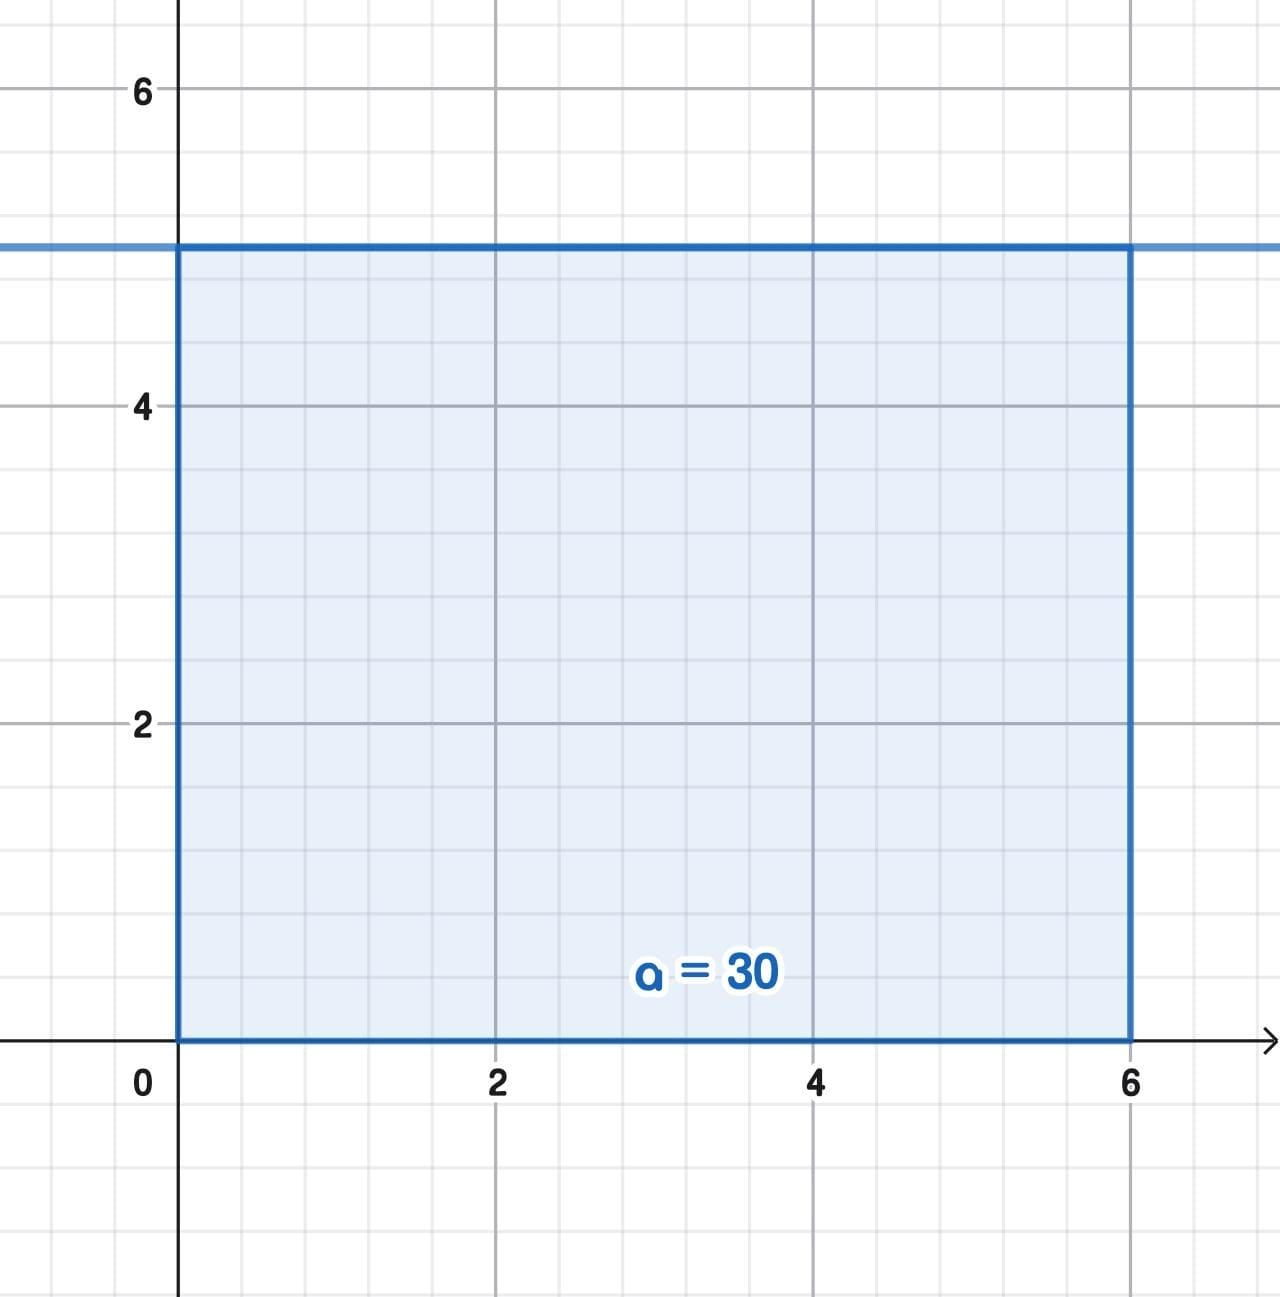
\includegraphics[width=0.86\textwidth]{imagenes/tema10_1_c.jpeg}
  \end{center}
  \newpage
  \item $\displaystyle\int_{-3}^3(-x+1)\,dx$. La integral con signo es
  \[
  \begin{aligned}
  \int_{-3}^3(-x+1)\,dx&=\left[-\frac{x^2}{2}+x\right]_{-3}^3\\
  &=\left(-\frac{3^2}{2}+3\right)-\left(-\frac{(-3)^2}{2}-3\right)\\
  &=\left(-\frac92+3\right)-\left(-\frac92-3\right)\\
  &=-\frac32+\frac{15}{2}=\boxed{6}.
  \end{aligned}
  \]
  Para distinguir el área geométrica total: de $-3$ a $1$ hay un trapecio de área $8$ y de $1$ a $3$ un triángulo debajo del eje $x$ de área $2$; el área geométrica total es $8+2=10$, mientras que el área con signo es $8-2=6$.
  \begin{center}
  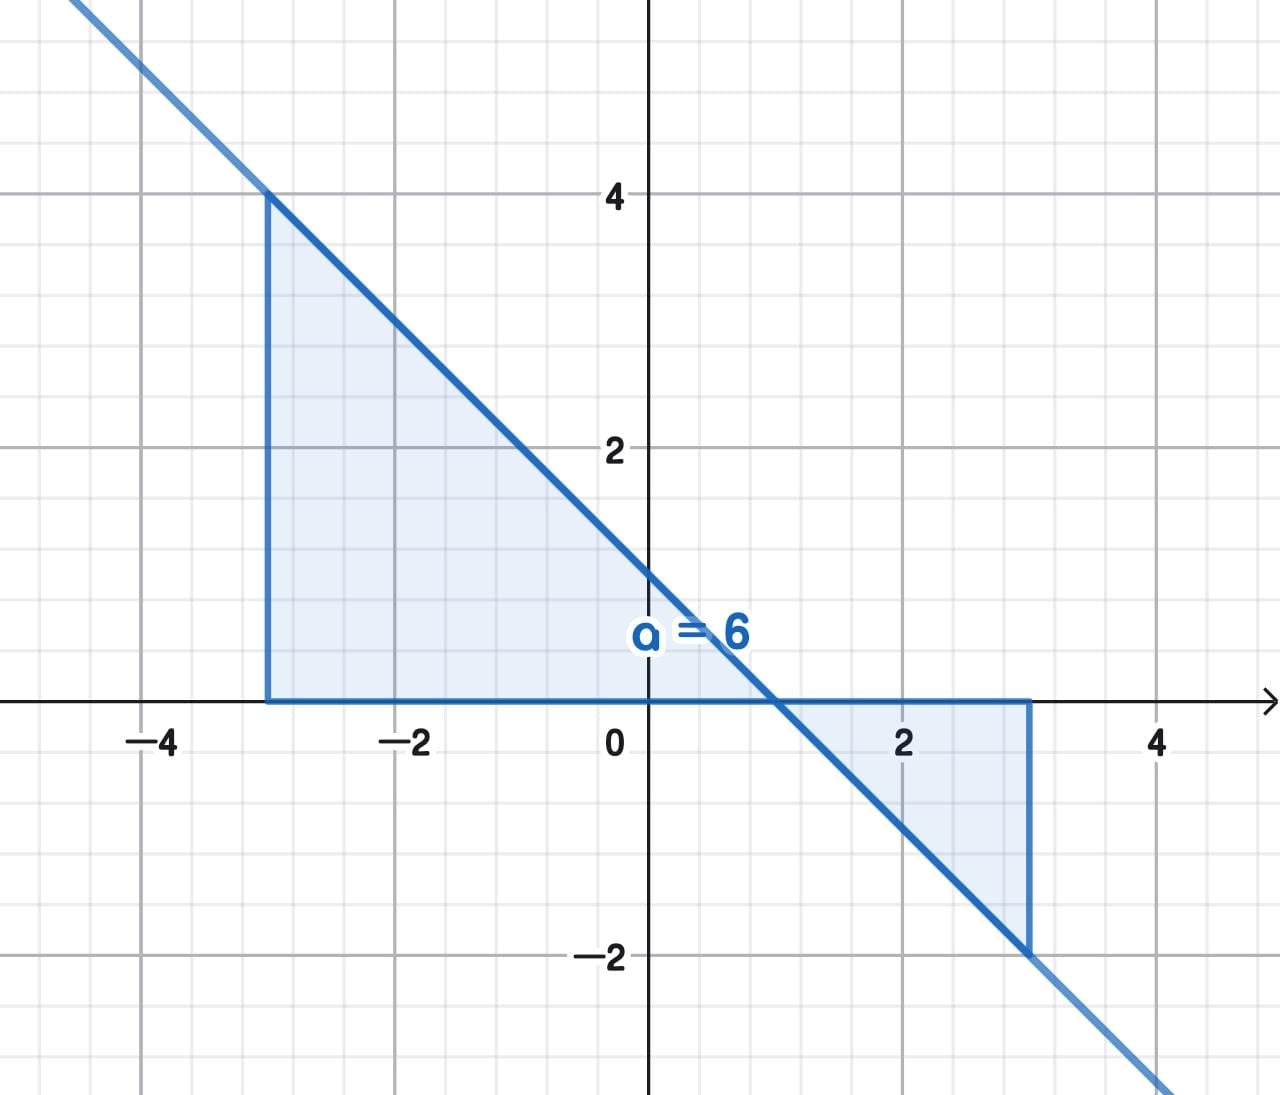
\includegraphics[width=0.86\textwidth]{imagenes/tema10_1_d.jpeg}
  \end{center}
  \newpage
  \item $\displaystyle\int_0^{2\pi}\sin x\,dx$. Primero recordamos que la integral de seno es $-\cos x$.
  \[
  \begin{aligned}
  \int_0^{2\pi}\sin x\,dx&=[-\cos x]_0^{2\pi}\\
  &=-\cos(2\pi)-(-\cos(0))\\
  &=-1-(-1)=\boxed{0}.
  \end{aligned}
  \]
  El área geométrica sin signo es $2+2=4$: dos regiones iguales, una sobre el eje $x$ y otra debajo.
  \begin{center}
  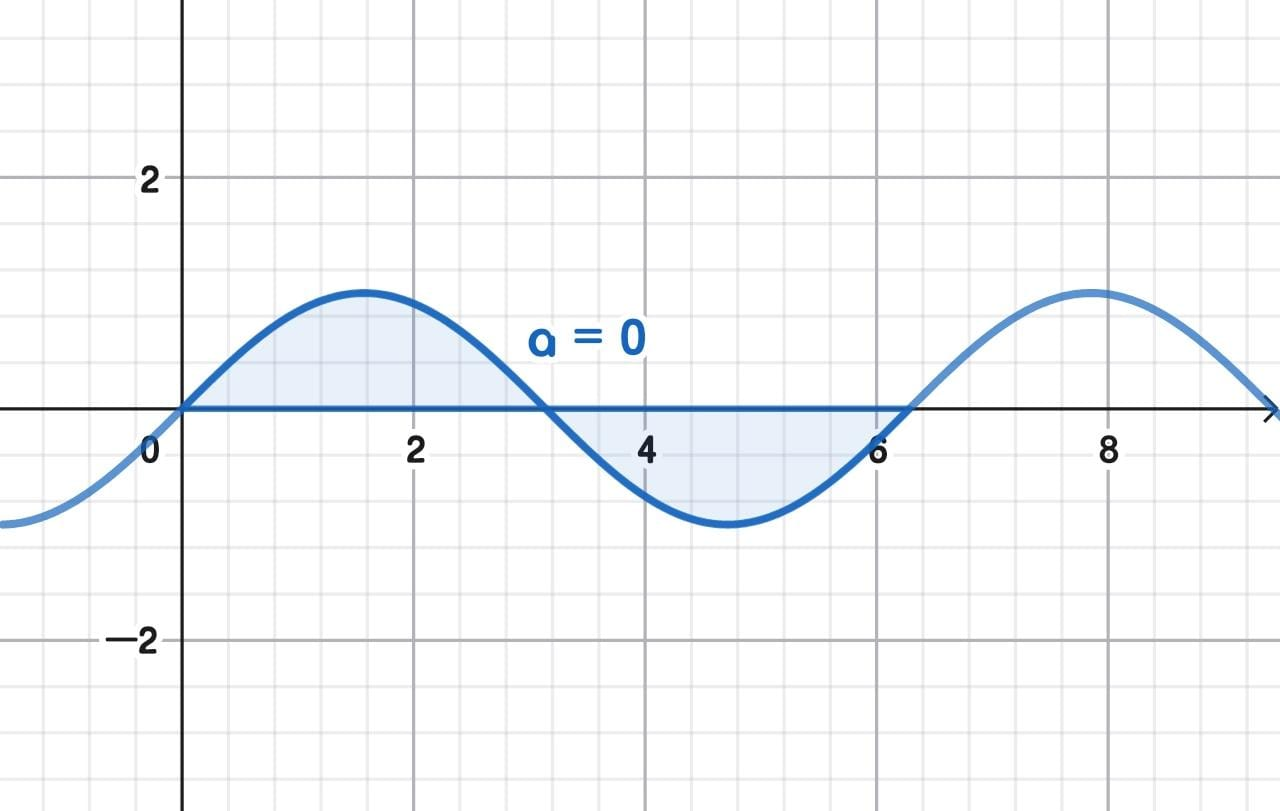
\includegraphics[width=0.86\textwidth]{imagenes/tema10_1_e.jpeg}
  \end{center}
\end{enumerate}

\subsection*{2.- Resuelve las siguientes integrales inmediatas:}
\begin{enumerate}[label=\alph*)]
  \item $\displaystyle\int(3x^2+\cos x)\,dx$. Separamos porque la integral de una suma es la suma de las integrales. Para $3x^2$, aumentamos el exponente y dividimos entre el exponente nuevo:
  \[
  \begin{aligned}
  \int(3x^2+\cos x)\,dx&=3\int x^2\,dx+\int\cos x\,dx\\
  &=3\left(\frac{x^3}{3}\right)+\sin x\\
  &=x^3+\sin x+C=\boxed{x^3+\sin x+C}.
  \end{aligned}
  \]
  \item $\displaystyle\int(e^x-\sin x)\,dx$. Integramos cada parte por separado; la integral de $-\sin x$ es $\cos x$ porque su derivada es $-\sin x$:
  \[
  \begin{aligned}
  &=\int e^x\,dx-\int\sin x\,dx\\
  &=e^x-(-\cos x)\\
  &=\boxed{e^x+\cos x+C}.
  \end{aligned}
  \]
  \item $\displaystyle\int(4\cos x+5\sin x)\,dx$. Los números 4 y 5 se pueden dejar afuera de las integrales:
  \[
  \begin{aligned}
  &=4\int\cos x\,dx+5\int\sin x\,dx\\
  &=4\sin x+5(-\cos x)\\
  &=\boxed{4\sin x-5\cos x+C}.
  \end{aligned}
  \]
  \item $\displaystyle\int\left(x^3+\frac12x^2+\frac{2}{\sqrt3}x+4\right)dx$. Vamos término por término y aplicamos la regla de aumentar el exponente en uno y dividir entre ese nuevo exponente:
  \[
  \begin{aligned}
  &=\frac{x^4}{4}+\frac12\frac{x^3}{3}+\frac{2}{\sqrt3}\frac{x^2}{2}+4x+C\\
  &=\boxed{\frac{x^4}{4}+\frac{x^3}{6}+\frac{x^2}{\sqrt3}+4x+C}.
  \end{aligned}
  \]
  \item $\displaystyle\int\left(3\sqrt{x}-5\sqrt[5]{x}\right)dx$. Primero escribimos las raíces como potencias: $\sqrt{x}=x^{1/2}$ y $\sqrt[5]{x}=x^{1/5}$:
  \[
  \begin{aligned}
  &=\int(3x^{1/2}-5x^{1/5})dx\\
  &=3\frac{x^{3/2}}{3/2}-5\frac{x^{6/5}}{6/5}\\
  &=2x^{3/2}-\frac{25}{6}x^{6/5}+C\\
  &=\boxed{2x^{3/2}-\frac{25}{6}x^{6/5}+C}.
  \end{aligned}
  \]
  \item $\displaystyle\int\left(\frac3{x^5}+\frac4{x^2}+\frac5x\right)dx$. Convertimos las fracciones a potencias negativas y aplicamos la regla de potencias. Para $1/x$, usamos que su integral es el logaritmo:
  \[
  \begin{aligned}
  &=\int(3x^{-5}+4x^{-2}+5x^{-1})dx\\
  &=3\frac{x^{-4}}{-4}+4\frac{x^{-1}}{-1}+5\ln|x|+C\\
  &=\boxed{-\frac{3}{4x^4}-\frac4x+5\ln|x|+C}.
  \end{aligned}
  \]
  \item $\displaystyle\int\frac5{\sqrt[3]{x^2}}dx$. La raíz se escribe como una potencia: $\sqrt[3]{x^2}=x^{2/3}$:
  \[
  \begin{aligned}
  &=5\int x^{-2/3}dx\\
  &=5\frac{x^{1/3}}{1/3}=15x^{1/3}\\
  &=\boxed{15\sqrt[3]{x}+C}.
  \end{aligned}
  \]
  \item $\displaystyle\int(2\tan x-3\sin x)dx$. Como $\tan x=\sin x/\cos x$, para la primera parte hacemos un cambio: $u=\cos x$, entonces $du=-\sin x\,dx$ y $\sin x\,dx=-du$:
  \[
  \begin{aligned}
  &=2\int\frac{\sin x}{\cos x}dx-3\int\sin x\,dx\\
  &=2\int\frac{-du}{u}+3\cos x+C\\
  &=-2\ln|u|+3\cos x+C\\
  &=-2\ln|\cos x|+3\cos x+C\\
  &=\boxed{-2\ln|\cos x|+3\cos x+C}.
  \end{aligned}
  \]
  \item $\displaystyle\int\left(\frac3{1+x^2}+\frac4{\sqrt{1-x^2}}\right)dx$. Reconocemos dos fórmulas: la integral de $1/(1+x^2)$ es $\arctan x$ y la de $1/\sqrt{1-x^2}$ es $\arcsin x$:
  \[
  \begin{aligned}
  &=3\int\frac{dx}{1+x^2}+4\int\frac{dx}{\sqrt{1-x^2}}\\
  &=3\arctan x+4\arcsin x+C\\
  &=\boxed{3\arctan x+4\arcsin x+C}.
  \end{aligned}
  \]
  \item $\displaystyle\int\left(\frac5{x^2-4}+\frac4{x\sqrt{x^2-9}}\right)dx$. Primero factorizamos $x^2-4=(x-2)(x+2)$ y acomodamos la primera fracción:
  \[
  \begin{aligned}
  \frac5{x^2-4}&=\frac5{(x-2)(x+2)}\\
  &=\frac54\left(\frac1{x-2}-\frac1{x+2}\right).
  \end{aligned}
  \]
  Integramos las dos partes. En la segunda usamos la fórmula correspondiente para $\int dx/(x\sqrt{x^2-a^2})$:
  \[
  \begin{aligned}
  &=\frac54\int\left(\frac1{x-2}-\frac1{x+2}\right)dx+4\int\frac{dx}{x\sqrt{x^2-9}}\\
  &=\frac54(\ln|x-2|-\ln|x+2|)+\frac43\arcsec\left(\frac{|x|}{3}\right)+C\\
  &=\boxed{\frac54\ln\left|\frac{x-2}{x+2}\right|+\frac43\arcsec\left(\frac{|x|}{3}\right)+C}.
  \end{aligned}
  \]
\end{enumerate}


% =================================================
% TEMA 11
% =================================================

\newpage
\section{Tema 11. Técnicas de integración: integración por cambio de variable e integración por partes}

\subsection{1.- Resuelve utilizando el método de integración por cambio de variable:}
\begin{enumerate}[label=\alph*)]
  \item $\displaystyle\int2x\sin(x^2)dx$. Dentro del seno está $x^2$ y afuera aparece $2x$, que es justo lo que sale al derivar $x^2$. Tomamos $u=x^2$, entonces $du=2x\,dx$:
  \[
  \begin{aligned}
  &=\int\sin u\,du\\
  &=-\cos u+C\\
  &=\boxed{-\cos(x^2)+C}.
  \end{aligned}
  \]
  \item $\displaystyle\int3x^2e^{x^3}dx$. Elegimos $u=x^3$ porque su derivada es $3x^2$ y ese factor está multiplicando:
  \[
  du=3x^2dx,\quad \int e^u du=e^u+C,\quad \boxed{e^{x^3}+C}.
  \]
  \item $\displaystyle\int x^2e^{x^3}dx$. El cambio sigue siendo $u=x^3$, pero ahora tenemos solamente $x^2dx$. Como $du=3x^2dx$, despejamos $x^2dx=du/3$:
  \[
  \begin{aligned}
  &=\frac13\int e^u du=\frac13e^u+C\\
  &=\boxed{\frac13e^{x^3}+C}.
  \end{aligned}
  \]
  \item $\displaystyle\int x\sin(x^2)dx$. Tomamos $u=x^2$ y $du=2x\,dx$. Como solo hay $x\,dx$, lo cambiamos por $du/2$:
  \[
  \begin{aligned}
  &=\frac12\int\sin u\,du\\
  &=-\frac12\cos u+C\\
  &=\boxed{-\frac12\cos(x^2)+C}.
  \end{aligned}
  \]
  \item $\displaystyle\int e^{-2x}dx$. La derivada de $-2x$ es $-2$, por eso al integrar debemos compensar dividiendo entre $-2$:
  \[
  \boxed{-\frac12e^{-2x}+C}.
  \]
  \item $\displaystyle\int\frac1{5-3x}dx$. Ponemos $u=5-3x$; al derivar $du=-3dx$, entonces $dx=-du/3$:
  \[
  \begin{aligned}
  &= -\frac13\int\frac1u du\\
  &=-\frac13\ln|u|+C\\
  &=\boxed{-\frac13\ln|5-3x|+C}.
  \end{aligned}
  \]
  \item $\displaystyle\int\frac{x^2}{x^3+1}dx$. Usamos $u=x^3+1$; su derivada es $3x^2$, así que $x^2dx=du/3$:
  \[
  \begin{aligned}
  &=\frac13\int\frac1u du\\
  &=\frac13\ln|u|+C\\
  &=\boxed{\frac13\ln|x^3+1|+C}.
  \end{aligned}
  \]
  \item $\displaystyle\int\frac{(\ln x)^2}{x}dx$. Como la derivada de $\ln x$ es $1/x$, hacemos $u=\ln x$, $du=dx/x$:
  \[
  \begin{aligned}
  &=\int u^2du=\frac{u^3}{3}+C\\
  &=\boxed{\frac{(\ln x)^3}{3}+C}.
  \end{aligned}
  \]
  \item $\displaystyle\int(x+1)\sqrt{2x+x^2}\,dx$. Lo que está dentro de la raíz es $x^2+2x$ y su derivada es $2x+2=2(x+1)$. Tomamos $u=x^2+2x$, por lo que $du=2(x+1)dx$ y $(x+1)dx=du/2$:
  \[
  \begin{aligned}
  &=\frac12\int u^{1/2}du\\
  &=\frac12\frac{u^{3/2}}{3/2}+C=\frac13u^{3/2}+C\\
  &=\boxed{\frac13(2x+x^2)^{3/2}+C}.
  \end{aligned}
  \]
  \item $\displaystyle\int(\cos^4\theta)(\sin\theta)d\theta$. Elegimos $u=\cos\theta$, entonces $du=-\sin\theta d\theta$. El signo menos aparece al sustituir:
  \[
  \begin{aligned}
  &=-\int u^4du\\
  &=-\frac{u^5}{5}+C\\
  &=\boxed{-\frac15\cos^5\theta+C}.
  \end{aligned}
  \]
  \item $\displaystyle\int\frac{e^u}{(1-e^u)^2}du$. Sea $v=1-e^u$. Al derivar, $dv=-e^u du$, por eso $e^u du=-dv$:
  \[
  \begin{aligned}
  &=-\int\frac1{v^2}dv=-\int v^{-2}dv\\
  &=-\frac{v^{-1}}{-1}+C=\frac1v+C\\
  &=\boxed{\frac1{1-e^u}+C}.
  \end{aligned}
  \]
  \item $\displaystyle\int_0^1\cos\left(\frac{\pi t}{2}\right)dt$. La integral de $\cos(kt)$ es $\sin(kt)/k$, por lo que aquí dividimos entre $\pi/2$:
  \[
  \begin{aligned}
  &=\left[\frac2\pi\sin\left(\frac{\pi t}{2}\right)\right]_0^1\\
  &=\frac2\pi\sin\left(\frac\pi2\right)-\frac2\pi\sin(0)\\
  &=\frac2\pi(1)-\frac2\pi(0)=\boxed{\frac2\pi}.
  \end{aligned}
  \]
\end{enumerate}


\subsection{2.- Resuelve utilizando el método de integración por partes:}
Se utiliza $\displaystyle\int u\,dv=uv-\int v\,du$. La idea es escoger una parte que sea fácil de derivar y otra que sea fácil de integrar.
\begin{enumerate}[label=\alph*)]
  \item $\displaystyle\int x\cos5x\,dx$. Tomamos $u=x$, así $du=dx$; y $dv=\cos5x\,dx$, entonces $v=\sin5x/5$:
  \[
  \begin{aligned}
  &=\frac{x\sin5x}{5}-\int\frac{\sin5x}{5}dx\\
  &=\frac{x\sin5x}{5}+\frac{\cos5x}{25}+C\\
  &=\boxed{\frac{x\sin5x}{5}+\frac{\cos5x}{25}+C}.
  \end{aligned}
  \]
  \item $\displaystyle\int te^{-3t}dt$. Elegimos $u=t$, $du=dt$; $dv=e^{-3t}dt$, cuya integral es $v=-e^{-3t}/3$:
  \[
  \begin{aligned}
  &= -\frac{te^{-3t}}3-\int\left(-\frac{e^{-3t}}3\right)dt\\
  &= -\frac{te^{-3t}}3-\frac{e^{-3t}}9+C\\
  &=\boxed{-\frac{te^{-3t}}3-\frac{e^{-3t}}9+C}.
  \end{aligned}
  \]
  \item $\displaystyle\int(x^2+2x)\cos x\,dx$. Separamos la suma y aplicamos partes a cada término, o lo hacemos con $u=x^2+2x$ y $dv=\cos xdx$:
  \[
  \begin{aligned}
  &= (x^2+2x)\sin x-\int(2x+2)\sin x\,dx\\
  &=(x^2+2x)\sin x-\left(-2x\cos x+2\sin x-2\cos x\right)\\
  &=(x^2+2x)\sin x+2x\cos x-2\sin x+2\cos x+C\\
  &=\boxed{(x^2+2x-2)\sin x+(2x+2)\cos x+C}.
  \end{aligned}
  \]
  \item $\displaystyle\int x^2\ln x\,dx$. Tomamos $u=\ln x$ y $dv=x^2dx$. Entonces $du=dx/x$ y $v=x^3/3$:
  \[
  \begin{aligned}
  &=\frac{x^3}{3}\ln x-\int\frac{x^3}{3}\frac1x dx\\
  &=\frac{x^3}{3}\ln x-\frac13\int x^2dx\\
  &=\frac{x^3}{3}\ln x-\frac{x^3}{9}+C\\
  &=\boxed{\frac{x^3}{3}\ln x-\frac{x^3}{9}+C}.
  \end{aligned}
  \]
  \item $\displaystyle\int(\ln x)^2dx$. Primero tomamos $u=(\ln x)^2$ y $dv=dx$, de modo que $du=2\ln x\,dx/x$ y $v=x$:
  \[
  \begin{aligned}
  &=x(\ln x)^2-2\int\ln x\,dx\\
  \end{aligned}
  \]
  Para la integral que quedó, hacemos partes otra vez: $u=\ln x$, $dv=dx$, entonces $du=dx/x$ y $v=x$; así $\int\ln xdx=x\ln x-x$.
  \[
  \begin{aligned}
  &=x(\ln x)^2-2(x\ln x-x)+C\\
  &=\boxed{x(\ln x)^2-2x\ln x+2x+C}.
  \end{aligned}
  \]
  \item $\displaystyle\int\sqrt{x^3}\ln x\,dx=\int x^{3/2}\ln x\,dx$. Escribimos la raíz como potencia y usamos partes: $u=\ln x$, $dv=x^{3/2}dx$. Entonces $du=dx/x$ y $v=\frac25x^{5/2}$:
  \[
  \begin{aligned}
  &=\frac25x^{5/2}\ln x-\frac25\int x^{3/2}dx\\
  &=\frac25x^{5/2}\ln x-\frac25\left(\frac25x^{5/2}\right)+C\\
  &=\boxed{\frac25x^{5/2}\ln x-\frac4{25}x^{5/2}+C}.
  \end{aligned}
  \]
  \item $\displaystyle\int x^3\sin x\,dx$. Aplicamos partes: $u=x^3$, $dv=\sin xdx$, por lo que $du=3x^2dx$, $v=-\cos x$:
  \[
  \begin{aligned}
  &=-x^3\cos x+3\int x^2\cos xdx\\
  \end{aligned}
  \]
  A la integral restante le aplicamos partes con $u=x^2$, $dv=\cos xdx$; después repetimos con $x$:
  \[
  \begin{aligned}
  \int x^2\cos xdx&=x^2\sin x-2\int x\sin xdx\\
  \int x\sin xdx&=-x\cos x+\sin x.
  \end{aligned}
  \]
  Sustituimos ambas expresiones:
  \[
  \begin{aligned}
  &=-x^3\cos x+3x^2\sin x-6(-x\cos x+\sin x)+C\\
  &=\boxed{-x^3\cos x+3x^2\sin x+6x\cos x-6\sin x+C}.
  \end{aligned}
  \]
  \item $\displaystyle\int x^5e^{-x}dx$. Usamos partes varias veces, siempre tomando $u$ como la potencia de $x$ (que va bajando) y derivándola. Al integrar $e^{-x}$ obtenemos $-e^{-x}$:
  \[
  \begin{aligned}
  &= -x^5e^{-x}+5\int x^4e^{-x}dx\\
  &= -x^5e^{-x}-5x^4e^{-x}+20\int x^3e^{-x}dx\\
  &= -x^5e^{-x}-5x^4e^{-x}-20x^3e^{-x}+60\int x^2e^{-x}dx\\
  &= -x^5e^{-x}-5x^4e^{-x}-20x^3e^{-x}-60x^2e^{-x}+120\int xe^{-x}dx\\
  &= -x^5e^{-x}-5x^4e^{-x}-20x^3e^{-x}-60x^2e^{-x}-120xe^{-x}-120e^{-x}+C\\
  &=\boxed{-e^{-x}(x^5+5x^4+20x^3+60x^2+120x+120)+C}.
  \end{aligned}
  \]
  \item $\displaystyle\int e^x\cos x\,dx$. Hacemos partes dos veces. Sea $I$ la integral que queremos resolver. La primera vez:
  \[
  I=e^x\sin x-\int e^x\sin xdx.
  \]
  La integral restante también por partes da $\int e^x\sin xdx=e^x\sin x-e^x\cos x+I$ al ordenar la igualdad. Sustituyendo y juntando la $I$ que aparece de nuevo:
  \[
  \begin{aligned}
  I&=e^x\sin x-(e^x\sin x-e^x\cos x-I)\\
  2I&=e^x(\sin x+\cos x)\\
  I&=\boxed{\frac{e^x}{2}(\sin x+\cos x)+C}.
  \end{aligned}
  \]
  \item $\displaystyle\int\sin(\ln x)dx$. Hacemos $u=\ln x$, así $x=e^u$ y $dx=e^u du$. Entonces queda $\int e^u\sin udu$, que es del mismo tipo que el ejercicio anterior; al regresar a $x$:
  \[
  \boxed{\frac{x}{2}\left[\sin(\ln x)-\cos(\ln x)\right]+C}.
  \]
\end{enumerate}


% =================================================
% TEMA 12
% =================================================

\newpage
\section{Tema 12. Técnicas de integración: integración de funciones trigonométricas e integración de funciones racionales}


\subsection{1.- Integra las siguientes funciones trigonométricas:}
\begin{enumerate}[label=\alph*)]
  \item $\displaystyle\int\cos^7x\,dx$. Separamos un coseno porque la potencia es impar; el resto lo cambiamos usando $\cos^2x=1-\sin^2x$. Luego tomamos $u=\sin x$, $du=\cos xdx$:
  \[
  \begin{aligned}
  &=\int\cos^6x\cos xdx=\int(1-\sin^2x)^3\cos xdx\\
  &\xrightarrow{u=\sin x}\int(1-u^2)^3du\\
  &=\int(1-3u^2+3u^4-u^6)du\\
  &=u-u^3+\frac35u^5-\frac17u^7+C\\
  &=\boxed{\sin x-\sin^3x+\frac35\sin^5x-\frac17\sin^7x+C}.
  \end{aligned}
  \]
  \item $\displaystyle\int(\sin^4x)(\cos^3x)dx$. Como la potencia del coseno es impar, dejamos un $\cos x$ y convertimos el resto: $\cos^2x=1-\sin^2x$. Usamos $u=\sin x$:
  \[
  \begin{aligned}
  &=\int\sin^4x(1-\sin^2x)\cos xdx\\
  &\xrightarrow{u=\sin x}\int u^4(1-u^2)du=\int(u^4-u^6)du\\
  &=\frac{u^5}{5}-\frac{u^7}{7}+C\\
  &=\boxed{\frac{\sin^5x}{5}-\frac{\sin^7x}{7}+C}.
  \end{aligned}
  \]
  \item $\displaystyle\int\sin^5x\,dx$. Dejamos un seno y convertimos $\sin^2x=1-\cos^2x$. Con $u=\cos x$ y $du=-\sin xdx$:
  \[
  \begin{aligned}
  &=-\int(1-u^2)^2du=-\int(1-2u^2+u^4)du\\
  &=-u+\frac23u^3-\frac15u^5+C\\
  &=\boxed{-\cos x+\frac23\cos^3x-\frac15\cos^5x+C}.
  \end{aligned}
  \]
  \item $\displaystyle\int(\sin^3x)(\cos^4x)dx$. Dejamos un seno, escribimos $\sin^2x=1-\cos^2x$ y cambiamos $u=\cos x$:
  \[
  \begin{aligned}
  &=-\int(1-u^2)u^4du=-\int(u^4-u^6)du\\
  &=-\frac15u^5+\frac17u^7+C\\
  &=\boxed{-\frac15\cos^5x+\frac17\cos^7x+C}.
  \end{aligned}
  \]
  \item $\displaystyle\int\cos^4x\,dx$. Usamos $\cos^2x=(1+\cos2x)/2$ y elevamos al cuadrado:
  \[
  \begin{aligned}
  \cos^4x&=\left(\frac{1+\cos2x}{2}\right)^2\\
  &=\frac14(1+2\cos2x+\cos^22x)\\
  &=\frac14\left(1+2\cos2x+\frac{1+\cos4x}{2}\right)\\
  &=\frac{3+4\cos2x+\cos4x}{8}.
  \end{aligned}
  \]
  Ahora integramos término a término, recordando que al integrar $\cos2x$ dividimos entre 2 y al integrar $\cos4x$ entre 4:
  \[
  \boxed{\frac{3x}{8}+\frac{\sin2x}{4}+\frac{\sin4x}{32}+C}.
  \]
  \item $\displaystyle\int\sin^6x\,dx$. Aplicamos la identidad de reducción de potencia (se puede obtener usando $\sin^2x=(1-\cos2x)/2$ y multiplicando varias veces):
  \[
  \sin^6x=\frac{10-15\cos2x+6\cos4x-\cos6x}{32}.
  \]
  Integramos cada parte:
  \[
  \boxed{\frac{5x}{16}-\frac{15\sin2x}{64}+\frac{3\sin4x}{64}-\frac{\sin6x}{192}+C}.
  \]
  \item $\displaystyle\int(\sin^2x)(\cos^2x)dx$. Como $\sin2x=2\sin x\cos x$, elevamos al cuadrado y usamos $\cos4x=1-2\sin^22x$:
  \[
  \sin^2x\cos^2x=\frac14\sin^22x=\frac18(1-\cos4x).
  \]
  Así,
  \[
  \int\frac18(1-\cos4x)dx=\boxed{\frac{x}{8}-\frac{\sin4x}{32}+C}.
  \]
  \item $\displaystyle\int(\tan^4x)(\sec^4x)dx$. Escribimos una parte de $\sec^2x$ para que sea la derivada de $\tan x$. Como $\sec^2x=1+\tan^2x$, usamos $u=\tan x$, $du=\sec^2x dx$:
  \[
  \begin{aligned}
  &=\int\tan^4x(1+\tan^2x)\sec^2x dx\\
  &\xrightarrow{u=\tan x}\int u^4(1+u^2)du\\
  &=\int(u^4+u^6)du=\frac{u^5}{5}+\frac{u^7}{7}+C\\
  &=\boxed{\frac{\tan^5x}{5}+\frac{\tan^7x}{7}+C}.
  \end{aligned}
  \]
  \item $\displaystyle\int(\tan^3x)(\sec^5x)dx$. Separamos $\sec x\tan xdx$ porque la derivada de $\sec x$ es precisamente esa. El resto se cambia con $\tan^2x=\sec^2x-1$. Sea $u=\sec x$:
  \[
  \begin{aligned}
  &=\int\tan^2x\sec^4x(\sec x\tan xdx)\\
  &\xrightarrow{u=\sec x}\int(u^2-1)u^4du\\
  &=\int(u^6-u^4)du=\frac{u^7}{7}-\frac{u^5}{5}+C\\
  &=\boxed{\frac{\sec^7x}{7}-\frac{\sec^5x}{5}+C}.
  \end{aligned}
  \]
  \item $\displaystyle\int(\sin3x)(\cos4x)dx$. Usamos la identidad que transforma un producto en suma: $\sin A\cos B=\frac12[\sin(A+B)+\sin(A-B)]$. Con $A=3x$, $B=4x$:
  \[
  \sin3x\cos4x=\frac12(\sin7x+\sin(-x))=\frac12(\sin7x-\sin x).
  \]
  Integramos los dos senos, teniendo cuidado de dividir entre 7 en el primero:
  \[
  \begin{aligned}
  &=\frac12\int(\sin7x-\sin x)dx\\
  &=\frac12\left(-\frac{\cos7x}{7}+\cos x\right)+C\\
  &=\boxed{-\frac{\cos7x}{14}+\frac{\cos x}{2}+C}.
  \end{aligned}
  \]
\end{enumerate}

\subsection{2.- Integra las siguientes funciones racionales:}
\begin{enumerate}[label=\alph*)]
  \item $\displaystyle\int\frac{x^4+3x^2+x}{x-2}dx$. Como el grado de arriba es mayor, primero dividimos polinomios. Al dividir obtenemos $x^3+2x^2+7x+15$ y sobra 30, por lo que:
  \[
  \frac{x^4+3x^2+x}{x-2}=x^3+2x^2+7x+15+\frac{30}{x-2}.
  \]
  Ahora integramos cada término. La última fracción se integra como logaritmo:
  \[
  \begin{aligned}
  &=\int(x^3+2x^2+7x+15)dx+30\int\frac1{x-2}dx\\
  &=\frac{x^4}{4}+\frac{2x^3}{3}+\frac{7x^2}{2}+15x+30\ln|x-2|+C\\
  &=\boxed{\frac{x^4}{4}+\frac{2x^3}{3}+\frac{7x^2}{2}+15x+30\ln|x-2|+C}.
  \end{aligned}
  \]
  \item $\displaystyle\int\frac{x+12}{x^2+5x+6}dx$. Factorizamos el denominador: $x^2+5x+6=(x+2)(x+3)$. Como son dos factores sencillos, separamos la fracción en dos:
  \[
  \frac{x+12}{(x+2)(x+3)}=\frac{A}{x+2}+\frac{B}{x+3}.
  \]
  Multiplicamos todo por $(x+2)(x+3)$: $x+12=A(x+3)+B(x+2)$. Si $x=-2$, $10=A$; si $x=-3$, $9=-B$, así $B=-9$:
  \[
  \frac{x+12}{(x+2)(x+3)}=\frac{10}{x+2}-\frac9{x+3}.
  \]
  Integramos usando $\int dx/(x+a)=\ln|x+a|$:
  \[
  \boxed{10\ln|x+2|-9\ln|x+3|+C}.
  \]
  \item $\displaystyle\int\frac{2x+3}{x^3+x^2-6x}dx$. Sacamos $x$ como factor y factorizamos el resto: $x^3+x^2-6x=x(x^2+x-6)=x(x+3)(x-2)$. Separamos en fracciones:
  \[
  \frac{2x+3}{x(x+3)(x-2)}=\frac A x+\frac B{x-2}+\frac C{x+3}.
  \]
  Multiplicando por el denominador, $2x+3=A(x+3)(x-2)+Bx(x+3)+Cx(x-2)$. Sustituyendo $x=0,2,-3$ se obtiene $A=-1/2$, $B=7/10$ y $C=-1/5$:
  \[
  =-\frac1{2x}+\frac7{10(x-2)}-\frac1{5(x+3)}.
  \]
  Integramos cada fracción como logaritmo:
  \[
  \boxed{-\frac12\ln|x|+\frac7{10}\ln|x-2|-\frac15\ln|x+3|+C}.
  \]
  \item $\displaystyle\int\frac{x^2}{x^4-5x^2+4}dx$. Factorizamos pensando en $x^2$: $x^4-5x^2+4=(x^2-1)(x^2-4)=(x-1)(x+1)(x-2)(x+2)$. Después se separa en cuatro fracciones sencillas:
  \[
  \frac{x^2}{(x^2-1)(x^2-4)}=-\frac1{3(x+2)}+\frac1{6(x+1)}-\frac1{6(x-1)}+\frac1{3(x-2)}.
  \]
  Se integra cada una con el logaritmo natural, conservando los signos y coeficientes:
  \[
  \boxed{-\frac13\ln|x+2|+\frac16\ln|x+1|-\frac16\ln|x-1|+\frac13\ln|x-2|+C}.
  \]
  \item $\displaystyle\int\frac{x+1}{x^2-6x+9}dx$. El denominador es un cuadrado perfecto: $x^2-6x+9=(x-3)^2$. Podemos separar el numerador $x+1=(x-3)+4$:
  \[
  \frac{x+1}{(x-3)^2}=\frac{x-3}{(x-3)^2}+\frac4{(x-3)^2}=\frac1{x-3}+\frac4{(x-3)^2}.
  \]
  Integramos: el primero es logaritmo; el segundo es una potencia negativa, cuya integral baja un exponente:
  \[
  \begin{aligned}
  &=\ln|x-3|+4\int(x-3)^{-2}dx\\
  &=\ln|x-3|-\frac4{x-3}+C\\
  &=\boxed{\ln|x-3|-\frac4{x-3}+C}.
  \end{aligned}
  \]
  \item $\displaystyle\int\frac{x}{x^3-3x^2+3x-1}dx$. El denominador se reconoce como $(x-1)^3$, porque es el desarrollo de $(x-1)^3=x^3-3x^2+3x-1$. Reescribimos el numerador $x=(x-1)+1$:
  \[
  \begin{aligned}
  &=\int\frac{(x-1)+1}{(x-1)^3}dx\\
  &=\int\left(\frac1{(x-1)^2}+\frac1{(x-1)^3}\right)dx\\
  &=\int((x-1)^{-2}+(x-1)^{-3})dx\\
  &=-\frac1{x-1}-\frac1{2(x-1)^2}+C\\
  &=\boxed{-\frac1{x-1}-\frac1{2(x-1)^2}+C}.
  \end{aligned}
  \]
  \item $\displaystyle\int\frac{x+1}{x^3+2x}dx$. Sacamos $x$ como factor: $x^3+2x=x(x^2+2)$. Reescribimos el numerador para que coincida con los términos del denominador y separamos:
  \[
  \frac{x+1}{x(x^2+2)}=\frac1{2x}-\frac{x-2}{2(x^2+2)}.
  \]
  En el segundo término, separamos $x-2=x-0+(-2)$ y usamos que la derivada de $x^2+2$ es $2x$:
  \[
  \begin{aligned}
  &=\frac12\int\frac1x dx-\frac12\int\frac{x}{x^2+2}dx+\int\frac1{x^2+2}dx\\
  &=\frac12\ln|x|-\frac14\ln(x^2+2)+\frac1{\sqrt2}\arctan\left(\frac{x}{\sqrt2}\right)+C\\
  &=\boxed{\frac12\ln|x|-\frac14\ln(x^2+2)+\frac1{\sqrt2}\arctan\left(\frac{x}{\sqrt2}\right)+C}.
  \end{aligned}
  \]
  \item $\displaystyle\int\frac{x+1}{x^4+3x^2+2}dx$. Factorizamos como si fuera una cuadrática en $x^2$: $x^4+3x^2+2=(x^2+1)(x^2+2)$. Separamos en dos fracciones:
  \[
  \frac{x+1}{(x^2+1)(x^2+2)}=\frac{x+1}{x^2+1}-\frac{x+1}{x^2+2}.
  \]
  En cada fracción separamos la parte con $x$ (que da logaritmo al hacer $u=x^2+a$) y la parte constante (que da arctan):
  \[
  \begin{aligned}
  &=\frac12\ln(x^2+1)+\arctan x-\frac12\ln(x^2+2)-\frac1{\sqrt2}\arctan\left(\frac{x}{\sqrt2}\right)+C\\
  &=\boxed{\frac12\ln(x^2+1)+\arctan x-\frac12\ln(x^2+2)-\frac1{\sqrt2}\arctan\left(\frac{x}{\sqrt2}\right)+C}.
  \end{aligned}
  \]
  \item $\displaystyle\int\frac{x^3+1}{x^4+4x^2+4}dx$. El denominador es $(x^2+2)^2$. Separamos el numerador para que una parte sea $x(x^2+2)$ y así aparezca la derivada del denominador:
  \[
  \frac{x^3+1}{(x^2+2)^2}=\frac{x}{x^2+2}-\frac{2x-1}{(x^2+2)^2}.
  \]
  Integramos la primera parte con $u=x^2+2$. En la segunda, separamos $2x$ y $-1$; el término con $2x$ también se integra con el mismo cambio y el que tiene $1$ usa la fórmula de arctan:
  \[
  \begin{aligned}
  &=\frac12\ln(x^2+2)+\frac{x+4}{4(x^2+2)}+\frac1{4\sqrt2}\arctan\left(\frac{x}{\sqrt2}\right)+C\\
  &=\boxed{\frac12\ln(x^2+2)+\frac{x+4}{4(x^2+2)}+\frac1{4\sqrt2}\arctan\left(\frac{x}{\sqrt2}\right)+C}.
  \end{aligned}
  \]
  \item $\displaystyle\int\frac{3x+4}{(x+1)(x+2)^2}dx$. Como el denominador tiene un factor repetido, usamos tres partes: $A/(x+1)+B/(x+2)+C/(x+2)^2$. Al multiplicar por todo el denominador:
  \[
  3x+4=A(x+2)^2+B(x+1)(x+2)+C(x+1).
  \]
  Sustituyendo valores sencillos y comparando se obtiene $A=1$, $B=-1$ y $C=2$:
  \[
  \frac{3x+4}{(x+1)(x+2)^2}=\frac1{x+1}-\frac1{x+2}+\frac2{(x+2)^2}.
  \]
  Integramos cada término:
  \[
  \begin{aligned}
  &=\ln|x+1|-\ln|x+2|+2\int(x+2)^{-2}dx\\
  &=\ln|x+1|-\ln|x+2|-\frac2{x+2}+C\\
  &=\boxed{\ln|x+1|-\ln|x+2|-\frac2{x+2}+C}.
  \end{aligned}
  \]
\end{enumerate}


\end{document}